\documentclass[oneside,numbers,spanish,english]{ezthesis}
%% # Opciones disponibles para el documento #
%%
%% Las opciones con un (*) son las opciones predeterminadas.
%%
%% Modo de compilar:
%%   draft            - borrador con marcas de fecha y sin im'agenes
%%   draftmarks       - borrador con marcas de fecha y con im'agenes
%%   final (*)        - version final de la tesis
%%
%% Tama'no de papel:
%%   letterpaper (*)  - tama'no carta (Am'erica)
%%   a4paper          - tama'no A4    (Europa)
%%
%% Formato de impresi'on:
%%   oneside          - hojas impresas por un solo lado
%%   twoside (*)      - hijas impresas por ambos lados
%%
%% Tama'no de letra:
%%   10pt, 11pt, o 12pt (*)
%%
%% Espaciado entre renglones:
%%   singlespace      - espacio sencillo
%%   onehalfspace (*) - espacio de 1.5
%%   doublespace      - a doble espacio
%%
%% Formato de las referencias bibliogr'aficas:
%%   numbers          - numeradas, p.e. [1]
%%   authoryear (*)   - por autor y a'no, p.e. (Newton, 1997)
%%
%% Opciones adicionales:
%%   spanish         - tesis escrita en espa'nol
%%
%% Desactivar opciones especiales:
%%   nobibtoc   - no incluir la bibiolgraf'ia en el 'Indice general
%%   nofancyhdr - no incluir "fancyhdr" para producir los encabezados
%%   nocolors   - no incluir "xcolor" para producir ligas con colores
%%   nographicx - no incluir "graphicx" para insertar gr'aficos
%%   nonatbib   - no incluir "natbib" para administrar la bibliograf'ia

%% Paquetes adicionales requeridos se pueden agregar tambi'en aqu'i.
%% Por ejemplo:
%\usepackage{subfig}
%\usepackage{multirow}
\usepackage{appendix}
\usepackage[absolute,overlay]{textpos}
  \setlength{\TPHorizModule}{1mm}
  \setlength{\TPVertModule}{1mm}
\usepackage[utf8]{inputenc} 
\usepackage[spanish]{babel}
\usepackage[ notlof, notlot, nottoc]{tocbibind}
\renewcommand\tocbibname{Referencias}
%% # Datos del documento #
%% Nota que los acentos se deben escribir: \'a, \'e, \'i, etc.
%% La letra n con tilde es: \~n.

\author{Jorge Iván Durán Páez}
\title{Aplicación para la predicción de resultados en la prueba Saber 11\degree}
\supervisor{Director\\Edgar Alberto Molina Rojas\\\href{mailto:edgarmolina2@gmail.com}{edgarmolina2@gmail.com}\\Asesor\\David Alejandro Przybilla\\\href{mailto:dav.alejandro@gmail.com}{dav.alejandro@gmail.com}}
\institution{Universidad del Valle}
\faculty{Escuela de Ingeniería de Sistemas y Computación}
\department{Ingeniería de Sistemas \\ Tuluá - Valle}

%% # M'argenes del documento #
%% 
%% Quitar el comentario en la siguiente linea para austar los m'argenes del
%% documento. Leer la documentaci'on de "geometry" para m'as informaci'on.

\geometry{top=30mm,bottom=30mm,inner=30mm,outer=20mm}
%% Se definen las dos líneas siguientes para las funciones relacionadas con las subsubsecciones
\setcounter{secnumdepth}{3} % Para que ponga (1.1.1.1) en subsubsecciones...
\setcounter{tocdepth}{3} % Para que añada las subsubsecciones en el indice...

%% El siguiente comando agrega ligas activas en el documento para las
%% referencias cruzadas y citas bibliogr'aficas. Tiene que ser *la 'ultima*
%% instrucci'on antes de \begin{document}.
%%\hyperlinking
\usepackage{colortbl}
\usepackage[colorlinks=true,linkcolor=black,urlcolor=black, citecolor=black]{hyperref}
\usepackage{hyperref}
\usepackage{float}
\usepackage{footnote}
\makesavenoteenv{tabular}
\usepackage{tabularx}
\usepackage{lipsum}
\usepackage{ragged2e}
\usepackage{multirow}
\usepackage{amsmath}
\setlength{\parindent}{0pt}
\newcommand\portada{

\selectlanguage{spanish}
\begin{titlepage}
    \begin{center}
        \begin{center}
            \Huge \inserttitle
            \vfill
            {\large Autor \\ \Large \insertauthor \\}
            \large Código 200859307\vfill        
            \huge \insertinstitution \par
            \large  \insertfaculty \par
            \insertdepartment \par {2014}
        \end{center}
    \end{center}
\end{titlepage}
}
\newcommand\contraportada{
\begin{titlepage}

\begin{center}

{ \Huge \inserttitle }
\vfill
{\large Autor \\ \insertauthor \par}
\href{mailto:jorge.ivan.duran@correounivalle.edu.co}{jorge.ivan.duran@correounivalle.edu.co}
\\
{Código 200859307}
\vfill
\large {Trabajo de grado para optar por el título de Ingeniero de
            Sistemas}
\vfill
{\large \insertsupervisor \par}
\vfill
\insertinstitution \\
\insertfaculty \\
\insertdepartment \\
{2014}

\end{center}

\end{titlepage}
}
\usepackage{underscore}
\usepackage{longtable}
\renewcommand{\degree}{\ensuremath{^\circ}}

\begin{document}
\portada
\contraportada
\thispagestyle{fancy}
\pagenumbering{roman}
\setcounter{page}{3}

\begin{huge}
\textbf{Nota de aceptación}
\end{huge} 
\vfill
\begin{Large}
\begin{flushright}
\rule{100mm}{0.05mm}\\
\rule{100mm}{0.05mm}\\
\rule{100mm}{0.05mm}\\
\rule{100mm}{0.05mm}\\
\rule{100mm}{0.05mm}\\
\textbf{Presidente
del Jurado}\\[2.0cm]
\rule{100mm}{0.05mm}\\\textbf{Jurado 1}\vfill
\rule{100mm}{0.05mm}\\\textbf{Jurado 2}\vfill
\end{flushright}
\begin{flushleft}
\large \textbf{Tuluá, Enero de 2014}
\end{flushleft}
\end{Large}
\newpage

\selectlanguage{spanish}

\begin{abstract}
\thispagestyle{fancy}
\setcounter{page}{4}
\justifying
El proceso de minería de datos, que permite descubrir nuevo y útil conocimiento a partir del análisis exhaustivo de información recolectada en un cierto intervalo del tiempo, puede ser aplicado a distintos contextos de la vida cotidiana. Para el caso de estudio que se desarrolló durante este proyecto, el contexto fue la educación. Específicamente se planteó lograr predecir puntajes de la prueba Saber 11\degree \ desarrollada por el Instituto Colombiano para la Evaluación de la Educación (ICFES).

En este trabajo se presenta el desarrollo del proyecto de minería de datos, se usó como fuentes de información las bases de datos del ICFES, las cual contienen información histórica sobre resultados e información personal de los evaluados.

Como resultado final se presenta la aplicación web PrediXaber11, donde las personas pueden acceder y ejecutar consultas. La aplicación usará la información suministrada del evaluado para entregar los posibles resultados en cada una de las áreas académicas evaluadas por el ICFES.\\

Palabras clave: Minería de datos, Saber 11\degree, Aplicación Web, KDD, Weka, ICFES, Java.
\end{abstract}
\selectlanguage{spanish}
\thispagestyle{fancy}
\setcounter{page}{5}
\Huge \textbf{Dedicatoria}\\[3.5cm]
\normalsize
A mis padres, fuente de inspiración y fortaleza en cada uno de los proyectos que emprendo. A mi hermano, un compañero de lucha cuando los obstáculos aparecen y de diversión cuando la alegría nos encara. Y a los muy pocos, pero muy fieles amigos, que en el camino he encontrado. Siempre estarán y siempre estaré.
\begin{flushright}
\textbf{Jorge} \end{flushright}
\newpage



\thispagestyle{fancy}
\Huge \textbf{Agradecimientos}\\[3.5cm]
\normalsize
A la Universidad de Valle, por su proyecto de ofrecer carreras de nivel profesional en ciudades no capitales. A los profesores que más que ser eso, se convirtieron en compañeros de charlas incansables sobre nuestro entorno académico y profesional.
\\
A compañeros de estudio, presión, preocupación y alegría, que encontré en la universidad y que espero la vida nos encuentre de manera constante.
\\
Cada peldaño pisado para alcanzar la meta, requirió de muchas personas que se hace imposible recordar, así que simplemente: Gracias, a todo el que sienta que aporto a mi carrera.
\\






\tableofcontents
\listoffigures
\listoftables
%\noindent \Huge \textbf{Lista de Anexos}\\[1.0cm]
\chapter*{Lista de anexos}
\normalsize

\noindent Anexo A: Cómo se hace la clasificación de las instituciones educativas según categorías de rendimiento \\
Anexo B: Saber 11 - Diccionario de Datos\\
Anexo C: Algunos totales de Control. Prueba Saber 11 (Examen de Estado)\\
Anexo D: Anexo D - Orientaciones para el examen de Estado de la educación media\\

%% Los cap'itulos inician con \chapter{T'itulo}, estos aparecen numerados y
%% se incluyen en el 'indice general.
%%
%% Recuerda que aqu'i ya puedes escribir acentos como: 'a, 'e, 'i, etc.
%% La letra n con tilde es: 'n.
\pagenumbering{arabic}
\setcounter{page}{13}
\chapter{Introducción}
\section{Descripción general}
En el ámbito de la educación en Colombia, la prueba Saber 11\degree\footnote{\url{http://www2.icfes.gov.co/examenes/saber-11o}} es de gran importancia para medir la calidad de la enseñanza que se está impartiendo en los colegios del país. La prueba Saber 11\degree \ es mayoritariamente presentada por estudiantes de grado 11 de los colegios del país, pero no es exclusiva de estos, cualquier persona puede presentarla, siempre y cuando ya haya obtenido título de bachiller.

Los resultados que se obtienen en la prueba no han presentado mejorías importantes en los últimos 5 años \cite{key-1, key-2, key-3, key-4}, causando preocupación por la calidad de la educación media en Colombia.

En \cite{key-4} se presenta un análisis a los resultados obtenidos por los estudiantes del departamento de Valle del Cauca en las pruebas Saber 5\degree, 9\degree\footnote{\url{http://www2.icfes.gov.co/examenes/pruebas-saber}} y 11\degree. Para el caso de la prueba Saber 11\degree, se presentan los resultados obtenidos en los años de 2002 a 2009, una comparación de estos resultados con los del promedio nacional de cada una de las áreas evaluadas y la categorización\footnote{\url{ftp://ftp.icfes.gov.co/SABER11/SB11-CLASIFICACION-PLANTELES/Clasificacion\%20planteles\%20SB11.pdf}} de los colegios en los años 2010 y 2011.

En las conclusiones y recomendaciones incluidas en \cite{key-4}, se establece la necesidad de brindar una educación que sea pertinente con las deficiencias académicas de los estudiantes, para así poder emprender planes de mejoramiento en las instituciones educativas y reducir los bajos rendimientos en la prueba Saber 11\degree.

En el presente documento se presenta el desarrollo de la construcción de una aplicación, para lograr determinar cuáles son los posibles resultados que obtendrán los estudiantes que están próximos a presentar la prueba Saber 11\degree \ y así conocer las áreas académicas en las cuales pueden poseer deficiencias.

\section{Problema}
\subsection{Descripción del problema}
Para la construcción de una aplicación, que permita conocer previamente como podría ser el puntaje de un estudiante en una o varias de las áreas académicas evaluadas en la prueba Saber 11\degree, se cuenta con las bases de datos del ICFES\footnote{\url{ftp://ftp.icfes.gov.co/SABER11/}}\footnote{Estas bases de datos son de acceso gratuito pero previamente se deben registrar los datos personales en \url{http://64.76.89.156/index.php/bdicfes/solicitudregistro}, para poder acceder al ftp.}, que almacenan información histórica sobre aspectos personales de los evaluados como por ejemplo: calendario académico del colegio al cual pertenece, carácter académico del colegio, ubicación del colegio (departamento y municipio), valor mensual de la pensión del colegio, si el hogar cuenta con servicio de alcantarillado y recolección de basuras, cantidad de automóviles que poseen en el hogar, si tiene o no computador, cantidad de televisores en el hogar, etnia a la cual pertenece, genero, fecha de nacimiento, si trabaja o no, nivel de educación de los padres, ocupación de los padres, etc. Y además información sobre los puntajes obtenidos por ellos en las áreas académicas evaluadas\footnote{\url{ftp://ftp.icfes.gov.co/SABER11/SB11-Diccionario_de_Datos-v1-6.pdf}.}.

El ICFES suministra estas bases de datos en archivos de Access\footnote{\url{http://office.microsoft.com/es-es/access}}, un archivo por cada prueba realizada desde el año 2000 (se realizan 2 pruebas cada año), pero estas bases de datos no son homogéneas, ya que durante las 24 pruebas registradas hasta el momento, la información almacenada de los evaluados no se ha mantenido constante. Durante 12 años la información ha sido recolectada a partir de encuestas en las cuales no siempre se han realizado las mismas preguntas. Por ejemplo, el dato sobre el nivel educativo de los padres se registró durante los años 2000 a 2004, pero no se registró en los años 2005 a 2007 y en 2008 vuelve a registrarse hasta ahora. Además los tipos de datos también se han modificado a lo largo de los años, en la época de 2000 a 2004 el valor ``3'' indicaba que el nivel de estudio de los padres llegaba a básica primaria, pero desde 2008 hasta ahora existen los valores ``9'' y ``10'' que significan ``Primaria Completa'' y ``Primaria Incompleta'' respectivamente. Causando esto que dentro de las bases de datos se encuentren muchos valores nulos y una falta de concordancia con los tipos de datos en muchos de los 84 atributos que se almacenan en las 24 bases de datos.

Por consiguiente, en el proceso de construcción de una aplicación que permitiera conocer cómo serían los resultados de un estudiante al momento de presentar la prueba Saber 11\degree, fue necesario realizar la reestructuración de estas bases de datos, para que su información fuera concordante y no almacenara datos nulos, y así posteriormente utilizarlas como insumo en la construcción de la aplicación.
\subsection{Formulación del problema}
¿Cómo construir una aplicación de software, usando las bases de datos suministradas por el ICFES, que permita conocer previamente los resultados de un estudiante en la prueba Saber 11\degree?
\section{Justificación}
Los puntajes obtenidos en la prueba Saber 11\degree \ son de gran importancia tanto para los estudiantes que la presentan, como para las instituciones educativas y para el gobierno nacional de Colombia, ya que estos brindan una estimación de los indicadores de calidad de la educación media en el país\footnote{\url{http://www.icfes.gov.co/examenes/saber-11o/objetivos}}.
Un estudiante que desea continuar con su vida académica ingresando a la educación universitaria, se ve en la necesidad de obtener puntajes que le permitan no solo cumplir con los mínimos puntajes necesarios de inscripción en la carrera de su predilección, sino que también le permitan ingresar a esta en la universidad. 

En las instituciones educativas, alcanzar un nivel medio o alto en la clasificación otorgada por el ICFES es de gran importancia para su prestigio dentro de la sociedad académica, los colegios utilizan además estos puntajes como un indicador de autoevaluación para medir la calidad de sus prácticas pedagógicas. 

Como se puede observar en la educación media del país, prácticamente todos los involucrados obtienen beneficios si se mejoran los puntajes obtenidos en la prueba Saber 11\degree. Un primer paso para trabajar en estas mejoras es tener la capacidad de detectar las deficiencias de los estudiantes. Con la aplicación que se propone construir en este documento, se podría dar ese primer paso. 
\section{Objetivos}
\subsection{Objetivo general}
Desarrollar una aplicación que permita predecir los puntajes que obtendrá un estudiante en la prueba Saber 11\degree.
\subsection{Objetivos específicos}
\begin{enumerate}
\item Aplicar el proceso de extracción, transformación y carga (Extract, transform and load, ETL) a las bases de datos suministradas por el ICFES.
\item Construir un clasificador, utilizando técnicas de minería de datos, a partir de la información procesada.
\item Implementar una interfaz en donde los usuarios puedan realizar consultas parametrizadas.
\end{enumerate}
\subsection{Resultados Esperados}
En la tabla \ref{tab:cuadro1} se pueden observar cuales fueron los resultados que se deseaba obtener al momento de cumplir con cada uno de los objetivos planteados.
\begin{table}[!htb]
\centering
\begin{tabular}{|p{2.5cm}|m{13cm}|}
\hline
	\rowcolor[gray]{0.9} 
	\textbf{Objetivo Especifico} &
	\textbf{Resultados Esperados} \\ 
\hline 
1 & \begin{itemize} \item Bases de datos del ICFES, con estructuras homogéneas y sin datos nulos.
					\item Data mart construido con la información procesada en las bases de datos del ICFES.
	\end{itemize} \\
\hline
2 & \begin{itemize} \item Informe sobre algoritmos de clasificación en el proceso de descubrimiento del conocimiento.
					\item Selección del algoritmo de clasificación que mejor se adapta a la cantidad y el tipo de datos con los que se cuenta en el data mart.
					\item Clasificador construido en base a la selección hecha.
	\end{itemize} \\
\hline
3 & \begin{itemize} \item Documentación de los procesos de diseño, codificación y pruebas de la interfaz de consultas.
	\end{itemize} \\ 
\hline
\end{tabular}
\caption{Relación de los objetivos específicos con sus resultados esperados.}
\label{tab:cuadro1}
\end{table}
\section{Alcance}
La presente propuesta establece la construcción de una aplicación que, usando solamente la información almacenada en las bases de datos históricas del ICFES, logre entregar a los usuarios información sobre cómo podrían ser los puntajes que obtendrá un estudiante en cada una de las áreas académicas evaluadas en la prueba Saber 11\degree. 

Para que un usuario pueda conocer el posible resultado de un estudiante, deberá realizar una consulta en donde ingresará datos personales del estudiante, estos datos personales que se deben ingresar serán definidos en el proceso de construcción del clasificador, pero no serán distintos a los registrados en las bases de datos del ICFES.

Después de ser consultada la aplicación, la información que contendrá la respuesta estará constituida por los puntajes que podría obtener un estudiante en cada una de las áreas académicas evaluadas en la prueba Saber 11\degree: lenguaje, matemáticas, biología, química, física, filosofía, ciencias sociales e ingles.

El proyecto se desarrollará llevando a cabo la propuesta metodológica presentada por José Hernández en \cite{key-50}.
\section{Estructura del documento}
El documento se encuentra organizado de la siguiente manera:

En el Capítulo 2 se encuentra el marco conceptual y referencial en los que se fundamentó el desarrollo de este trabajo de grado.

En el Capítulo 3 se relaciona como se realizó el proceso de Extracción, Transformación y Carga de las bases de datos recolectadas.

En el Capítulo 4 se presentan los algoritmos de minería de datos, para la construcción de clasificadores, utilizados y los resultados obtenidos con cada uno de ellos.

En el Capítulo 5, se involucran los aspectos del desarrollo de la aplicación web construida para que los usuarios puedan realizar sus consultas.

En el Capítulo 6, se concluye el proyecto y se presentan las ideas para posibles trabajos futuros.
\chapter{Marco Referencial}
\section{Marco conceptual}
\subsection{Descubrimiento del conocimiento en bases de datos (KDD)}
En \cite{key-60} se define como: \begin{quote} Es el proceso de utilizar la información contenida en los sistemas de almacenamientos de datos para identificar patrones significativos, validos, novedosos, potencialmente útiles y comprensibles para el usuario. El proceso global consiste en transformar información de bajo nivel en conocimiento de alto nivel. El proceso KDD es interactivo e iterativo conteniendo los siguientes pasos: comprender el dominio de aplicación, extraer la base de datos objetivo, preparar los datos, minería de datos, interpretación y utilizar el conocimiento descubierto \end{quote}.
\subsection{Minería de datos}
En \cite{key-60} se define como: \begin{quote} Es un campo interdisciplinar con el objetivo general de predecir las salidas y revelar relaciones en los datos. Las tareas propias de la minería de datos pueden ser descriptivas, (i.e. descubrir patrones interesantes o relaciones describiendo los datos), o predictivas (i.e. clasificar nuevos datos basándose en los anteriormente disponibles). Para ello se utilizan herramientas automáticas que emplean algoritmos sofisticados para descubrir principalmente patrones ocultos, asociaciones, anomalías, y/o estructuras de la gran cantidad de datos almacenados en los Data Warehouses u otros repositorios de información, y filtran la información necesaria de las grandes bases de datos \end{quote}.
\subsection{Clasificación}
En la minería de datos, probablemente la tarea más popular por su objetivo es la clasificación. En esta tarea el objetivo es construir una función que permita, usando los atributos de una instancia, conocer la clase a la cual puede pertenecer la instancia. Para la construcción de los clasificadores se utiliza un conjunto de datos de entrenamiento, los cuales contiene un grupo de atributos predictores y un atributo a predecir, normalmente conocido como la clase a predecir. \\ \\
Formalmente, en \cite{key-70} se define como la tarea de aproximar una \emph{función objetivo} desconocida, que describe cómo instancias del problema deben ser clasificadas
de acuerdo a un experto en el dominio, \begin{quote}$\Phi:I\times C\rightarrow\left\{ T,F\right\} $\end{quote}
 por medio de una función llamada el \emph{clasificador}, \begin{quote}
$\Theta:I\times C\rightarrow\left\{ T,F\right\} $
\end{quote} 
 donde \begin{quote}
 $C=\left\{ c_{1},...,c_{|c|}\right\} $ es un conjunto de categorías predefinido\end{quote}
 e \begin{quote}\emph{I} es un conjunto
de instancias del problema\end{quote} Comúnmente cada instancia $i_{j}\epsilon I$
es representada como una lista $A=\left\{ a_{1},a_{2},...,a_{|A|}\right\} $
de valores característicos, conocidos como \emph{atributos}, i.e.
$i_{j}=\left\{ a_{1},a_{2},...,a_{|A|j}\right\} $. \\Si \begin{quote}$\Phi:i_{j}\times c_{i}\rightarrow T$,
entonces es llamado un ejemplo positivo de $c_{i}$ \end{quote} mientras si \begin{quote}$\Phi:i_{j}\times c_{i}\rightarrow F$
éste es llamado un ejemplo negativo de $c_{i}$\end{quote}

Para generar automáticamente el clasificador de $c_{i}$ es necesario
un proceso inductivo, llamado el \emph{aprendizaje}, el cual por observar
los atributos de un conjunto de instancias preclasificadas bajo $c_{i}$
o $\bar{c_{i}}$, adquiere los atributos que una instancia no vista
debe tener para pertenecer a la categoría. Por tal motivo, en la construcción
del clasificador se requiere la disponibilidad inicial de una colección
$\Omega$ de ejemplos tales que el valor de $\Phi\left(i_{j},c_{i}\right)$
es conocido para cada $\left\langle i_{j},c_{i}\right\rangle \epsilon\Omega\times C$.
A la colección usualmente se le llama \emph{conjunto de entrenamiento}
$\left(Tr\right)$.
\subsection{Evaluación de clasificadores}
Al momento de evaluar un clasificador, lo que se busca es conocer como es clasificada cada una de las instancias de un conjunto de evaluación. En estas instancias se conoce la clase a la cual pertenecen. El clasificador, procesa el conjunto de evaluación y retorna la clase a la que cada instancia debería pertenecer según los atributos predictores que contiene.\\
Usando las clasificaciones reales y las retornadas después de la evaluación, se generan 2 valores de evaluación de la calidad del clasificador. Estos 2 valores son Precisión y Exhaustividad (Presicion and Recall).\\
La precisión es la fracción de instancias correctamente clasificadas en una clase y la exhaustividad en la fracción de instancias de una clase que se clasificaron correctamente. \cite{key-280}\\
Teniendo que:
\begin{center}
$A=Conjunto\ de\  instancias\  de\  la\  clase\  X\  en\  el\  conjunto\  de\  evaluaci\acute{o}n$

$B=Conjunto\  de\  instancias\  clasificadas\  en\  la\  clase\  X\  por\  el\  clasificador$
\end{center}
Entonces
\begin{center}
$Presici\acute{o}n=\frac{|A\cap B|}{|B|}$

$Recall=\frac{|A\cap B|}{|A|}$
\end{center}
Cuanto más cerca estén estos valores a 1, mejor será la calidad del clasificador.
\subsection{ICFES}
Instituto Colombiano para la Evaluación de la Educación, entidad especializada en ofrecer servicios de evaluación de la educación en todos sus niveles, y en particular apoyar al Ministerio de Educación Nacional en la realización de los exámenes de Estado y en adelantar investigaciones sobre los factores que inciden en la calidad educativa, para ofrecer información pertinente y oportuna para contribuir al mejoramiento de la calidad de la educación en Colombia \cite{key-80}.
\subsection{Prueba Saber 11\degree}\label{sec:saber11}
Antes conocida como Examen del ICFES, es un examen de estado que evalúa a los estudiantes que están terminando su ciclo de Educación Media. La prueba tiene como finalidad apoyar los procesos de selección y admisión que realizan las instituciones de Educación Superior. Además de este propósito, la prueba busca:
\begin{itemize}
\item Brindar al estudiante información que contribuya a la selección de
su opción profesional. 
\item Proporcionar información a las instituciones de educación básica y
media sobre el desempeño de los estudiantes. 
\item Contribuir al desarrollo de estudios de tipo cultural, social y educativo. 
\item Servir de criterio para otorgar beneficios educativos. 
\end{itemize}
Las áreas académicas evaluadas actualmente por la prueba Saber 11\degree \ son:
\begin{itemize}
\item Lenguaje 
\item Matemáticas 
\item Biología 
\item Química 
\item Física 
\item Filosofía 
\item Ciencias sociales 
\item Inglés 
\item COMPONENTE FLEXIBLE (solo se presenta una de las siguientes opciones)
\begin{itemize}
\item Profundización en lenguaje 
\item Profundización en matemáticas 
\item Profundización en biología 
\item Profundización en ciencias sociales 
\item Interdisciplinar violencia y sociedad 
\item Interdisciplinar medio ambiente
\end{itemize}
\end{itemize}
\subsection{Data Warehouse}
Es un repositorio de datos operacionales seleccionados y adaptados subjetivamente, que puede responder consultas de tipo ad hoc, estadísticas o analíticas. Está situado en el centro de los sistemas de apoyo a la toma de decisiones de una organización y contiene datos históricos, resumidos y detallados de esta. Es esencial para una inteligencia de negocios efectiva, para la formulación e implementación de estrategias donde la gran cantidad de datos requieren ser procesados de manera rápida para comprender su significado e impacto. Permite una fácil organización y mantenimiento de los datos para una rápida recuperación y análisis de la manera en que sean requeridos \cite{key-90}.
\subsection{Data Mart}
Desde un Data Warehouse, los datos fluyen hacia los departamentos de la organización, que personalizan la información almacenada para que sea útil en los sistemas de información de cada uno de ellos. Estos componentes individuales con características personalizadas son conocidos como Data Mart. En otras palabras, es un cuerpo de datos de un sistema de información, que posee la estructura fundamental de un Data Warehouse, es una subsección de una Data Warehouse y más popular que este \cite{key-90}.
\section{Antecedentes o Estado del Arte}
En el área de la educación, los trabajos presentados a continuación se orientaron a encontrar posibilidades de bajos rendimiento académicos y así lograr conocer perfiles o factores que hacen que los estudiantes no logren las metas propuestas en sus estudios. Este trabajo de grado también se orientó a encontrar estas posibilidades de bajos rendimientos, pero no aplicado a estudiantes de universidades, sino a los estudiantes que presentan la prueba Saber 11\degree.

También se observó la variedad de algoritmos utilizados para construir los clasificadores, en algunos trabajos se utilizó más de un algoritmo para lograr encontrar comparaciones de rendimiento y mejores niveles de precisión con cada algoritmo. En este trabajo se evaluaron distintos algoritmos para la construcción de clasificadores, con el fin de encontrar información sobre cómo se comportan con la cantidad de datos usados y con la estructura que posean estos datos.

En este trabajo se utilizaron bases de datos que contenían más de 5 millones de registros\footnote{\url{ftp://ftp.icfes.gov.co/SABER11/SB11-FTP_Algunos_Totales_de_Control-v1-1.pdf}}, recolectados a lo largo de 11 años y que presentan una gran variación en la integridad de los atributos de estos registros. Por eso este trabajo centró su primera parte en la homogeneización de estas bases de datos. En los trabajos revisados, la cantidad de datos utilizados en los procesos de investigación, no eran tantos como los que se utilizaron en este trabajo.

En conclusión los trabajos aquí presentados sirvieron de base para la realización de este trabajo, ya que sus fases de investigación fueron las mismas en la mayoría de los trabajos, iguales a las que se aplicaron en este trabajo. Además, los resultados obtenidos en ellos, muestran la utilidad de la construcción de clasificadores para predecir resultados de estudiantes en exámenes o procesos de su vida académica.
\subsection{Detección de patrones de bajo rendimiento académico y deserción estudiantil con técnicas de minería de datos \cite{key-100}}
Su objetivo fue determinar en la comunidad universitaria perfiles de bajo rendimiento académico y deserción estudiantil aplicando técnicas de descubrimiento del conocimiento, a partir de los datos almacenados en las bases de datos durante los últimos 15 años. Este proceso se apoyó con TariyKDD\footnote{\url{http://developer.berlios.de/projects/tariykdd/}}, una herramienta de minería de datos de distribución libre. Aunque el trabajo de investigación este orientado a detectar bajos rendimientos de estudiantes en la universidad, su proceso de investigación es similar al que se espera llevar en este proyecto, por lo tanto sirve de guía para el desarrollo de este. Además de que la información utilizada para predecir el comportamiento académico de los estudiantes se basa en información socio-económica, que es la misma con la que se cuenta en las bases de datos del ICFES para construir el clasificador.

Este trabajo desarrolló de manera organizada y bien estructurada, cada uno de los pasos planteados en \cite{key-50}. El algoritmo de minería de datos utilizado fue arboles de clasificación con C4.5 \cite{key-50, key-70}, los resultados entregados por esta investigación mostraron cuales eran los perfiles de los estudiantes que podrían prever un bajo rendimiento.
La investigación se realizó en la Universidad de Nariño de Colombia. Las bases de datos recolectadas contenían información sobre el desempeño académico e información personal de 46173 estudiantes, acumuladas durante 15 años.

Inicialmente se contaba con 69 atributos en las bases de datos que describían las características de los estudiantes, pero después de pasar por el proceso de limpieza y transformación de los datos, y utilizando TariyKDD para seleccionar los atributos más relevantes, se llegó a una lista de 26 atributos y una cantidad de registros de 20329.

Finalmente, se aplicaron las técnicas de minería de datos para clasificación, en este caso el algoritmo C4.5 y se obtuvieron las reglas que indicaban que tipo de situaciones personales de un estudiante podrían llevar a obtener un bajo rendimiento en la universidad. Unos ejemplos de las reglas obtenidas son:
\begin{itemize}
\item Si el estrato socioeconómico es 2, el ponderado de exámenes de estado ICFES está entre 50 y 70, es del Sur de Nariño, está en primer semestre y pertenece a la facultad de Ciencias Humanas, entonces su rendimiento es Bajo. El 68\% con estas características se clasifican de esta manera. 
\item Si la edad de ingreso es menor o igual a 18 años, el estrato socioeconómico es 2, género masculino, el ponderado ICFES está entre 50 y 70, vive con la familia, es del Sur de Nariño, está en primer semestre, está en la facultad de Ciencias Naturales y Matemáticas, entonces su rendimiento es Bajo. El 67\% con estas características se clasifican de esta manera. 
\end{itemize}
\subsection{Minería de datos en la educación \cite{key-110}}
En este documento se describe el uso de la minería de datos aplicada a entornos educativos y su uso pedagógico. De manera muy clara y especifica brinda una vista de cómo se debe realizar un proceso de minería de datos en educación y su importancia.

Además muestra un ejemplo: ``Identificación de características de fracasos escolares en institutos''. En este se usan arboles de decisión porque permiten encontrar cuales son las variables que tienen mayor relación con la variable que se desea predecir. El algoritmo de árboles de decisión utilizado fue CHAID \cite{key-120} (Chi-Squared Automatic Interaction Detection). CHAID realiza comparaciones en pares para encontrar la variable de predicción más altamente relacionada con la variable raíz. En sistemas de muchas variables, tener esta función implementada en un ordenador es esencial para procesar amplios conjuntos de datos (Big Data) \cite{key-110}. El resultado entregado fue un árbol, el cual se debió analizar para determinar su información.
\subsection{Minería de datos: predicción de la deserción escolar mediante el algoritmo de árboles de decisión y el algoritmo de los k vecinos más cercanos \cite{key-130}}
Se aplicaron técnicas de minería de datos para buscar conocer previamente si los estudiantes eran propensos a abandonar su carrera en la Universidad Tecnológica de Izúcar de Matamoros, México, tomando como base de análisis los datos del estudio socioeconómico del EXANI-II\footnote{\url{http://www.ceneval.edu.mx/ceneval-web/content.do?page=1738}}, elaborado por el CENEVAL\footnote{\url{http://www.ceneval.edu.mx/ceneval-web/content.do?page=1702}}, mismo que se aplica desde el año 2003 en la institución. Para esta investigación se utilizaron específicamente dos algoritmos: el algoritmo de árboles de clasificación C4.5 y el algoritmo de los k vecinos más cercanos \cite{key-70}.

En el proceso de transformación de los datos, el más largo en muchos de los trabajos que se realizan, incluyendo este, se modificó e integró toda la información encontrada en distintos formatos de almacenamiento, además no tenía un estructura clara, porque constaba de información de estudiantes de 14 cuatrimestres, por supuesto en cada registro no se realizaban las mismas preguntas, además de que muchas de estas se pueden responder como ``No lo sé'', después de superar esta etapa y aplicar los algoritmos previstos, se encontró que el algoritmo de los k vecinos más cercanos funciona bien con pocos datos (477 instancias), pero al momento de probarlo con 6525 instancias, el algoritmo C4.5, tuvo resultados más confiables (98,98\%).

Aquí también se realizó la creación de una herramienta que pueda ser accedida por cualquier usuario y le informa sobre la probabilidad de que un estudiante deserte. Los resultados mostraron que la edad, la situación económica y el nivel de inglés, tienen fuerte relación con que el estudiante deserte de la universidad.
\subsection{Modelo predictivo para la determinación de causas de reprobación mediante minería de datos \cite{key-140}}
En este trabajo, realizado en la Universidad Tecnológica de Puebla, México, se llevó a cabo el análisis de los datos que permitirán generar un modelo que ayude a predecir, desde que los alumnos ingresan a la Universidad, las causas que los llevarán a reprobar, así como las materias con mayor riesgo de ser reprobadas.

El algoritmo de clasificación utilizado fue C4.5, y se recolectaron datos con información de todas las carreras ofrecidas por la universidad. Este proceso de nuevo fue demorado, porque sus fuentes de almacenamiento poseían distintas estructuras y no existía una homogeneidad en los datos.

Los resultados obtenidos mostraron que de las 157 materias distintas que ofrece la universidad en sus carreras, 64 materias tienen un porcentaje de reprobación menor a 40\% y por lo tanto no generan un árbol de predicción. En las materias con un porcentaje mayor al 50\% se determinó que el factor principal de reprobación es el profesor que imparte la materia y también la edad de los estudiantes.
\subsection{La metodología del Data Mining. Una aplicación al consumo de alcohol en adolescentes \cite{key-150}}
Aunque en esta investigación el objetivo no estaba focalizado en descubrir conocimiento en el área de la educación. Es un trabajo interesante el cual sirvió de guía en este trabajo de grado, ya que en él se realizó la construcción de 3 algoritmos distintos de predicción: redes neuronales, arboles de decisión y Naive Bayes \cite{key-50}.

El trabajo se centra en demostrar la importancia que tiene el descubrimiento del conocimiento en bases de datos al momento de predecir comportamientos en distintas áreas como educación, finanzas, comercio, telecomunicaciones, salud, entre otras.

Estos algoritmos fueron aplicados en un conjunto de datos que contenía 7030 registro que informaban sobre el consumo de alcohol en jóvenes de entre 14 y 18 años con una cantidad de 20 variables que incluían información de la personalidad como los constructos de autoestima, impulsividad, conducta antisocial y búsqueda de sensaciones.

Los mejores resultados se obtuvieron con el modelo construido con redes neuronales, 64,1\% de precisión al momento de predecir si un joven consumía o no alcohol. Los otros resultados fueron una precisión de 62,3\% con árboles de decisión usando el algoritmo CART \cite{key-50} y una precisión de 59,9\% usando Naive Bayes.
\section{Marco Teórico}
Para la realización de este trabajo se utilizó la propuesta de fases claramente establecidas en \cite{key-50} donde establece que: ``Este proceso es iterativo e interactivo. Es iterativo ya que la salida de alguna de las fases puede hacer volver a pasos anteriores y porque a menudo son necesarias varias iteraciones para extraer conocimiento de alta calidad. Es interactivo porque el usuario (experto en el dominio del problema) interviene en la toma de muchas decisiones''.

La teoría del proceso del desarrollo de un proyecto de descubrimiento del conocimiento en bases de datos, define los siguientes pasos:
\begin{figure}[H]
\begin{centering}
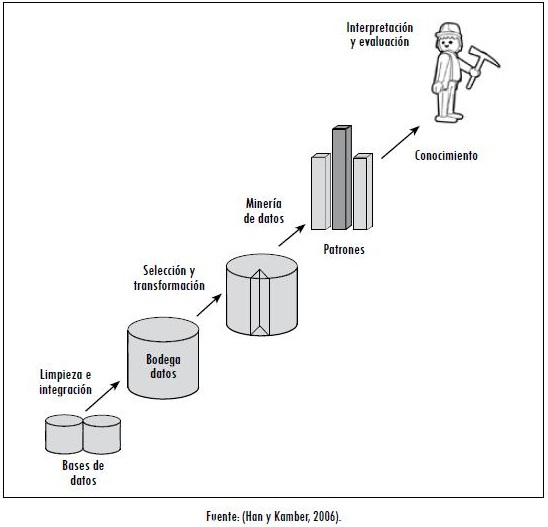
\includegraphics[scale=0.5]{v13n1a07-3}
\par\end{centering}
\caption{Proceso de descubrimiento del conocimiento en bases de datos.}
\end{figure}
\subsection{Selección (\emph{Extraction}) \cite{key-50,key-100}}
En esta etapa del proceso, es donde se investigan las fuentes, en las cuales se podrán encontrar los datos que me servirán para general un almacén de datos con información útil. Se recolectan todos los datos obtenidos en estas fuentes y se organizan en bases de datos que se usaran para la etapa de transformación.

Comúnmente en los trabajos orientados a la academia \cite{key-100, key-110, key-130, key-140}, estos datos son la información de los estudiantes de la institución a lo largo del tiempo. Los datos pueden incluir información acerca de la situación socio-económica del estudiante, sus notas, su entorno académico, información familiar, entre muchas otras que defina la institución que es importante recolectar.

En \cite{key-140}, donde se buscaba encontrar las reglas que indicaran si un estudiante era propenso a reprobar una materia, se seleccionaron como datos útiles: calificaciones por área del examen de admisión EXANI II, datos relevantes del estudio socio-económico, calificación del test de intereses vocacionales (KUDER), calificación del test de coeficiente intelectual (RAVEN), estilos de aprendizaje, evaluación a profesores, asignaturas cursadas y su promedio por cuatrimestre.
\subsection{Transformación (\emph{Transformation}) \cite{key-50,key-100}}
En esta etapa el proceso se basa en realizar primero una limpieza de los datos, la limpieza permite obtener datos sin valores nulos o anómalos, además se estandarizan los datos para que sean del mismo tipo. 

Para eliminar los datos nulos, se puede omitir este atributo o en algunos casos, cuando no son muchos los registros carentes de este valor, se pueden aplicar técnicas estadísticas como la media para insertar un valor valido y así no eliminar el registro o el atributo de la base de datos.

Estos procesos de limpieza, integración y agregación de los datos, entregan como resultado una base de datos modificada con los atributos relevantes en los registros, para responder al objetivo de la investigación, muchas veces esto genera que la cantidad de registros que se tenían inicialmente, se disminuya significativamente. Pero esto permitirá obtener resultados mucho más confiables, ya que no habrá datos que generen conflictos a la hora de generar clasificaciones con respecto a algunos atributos.
\subsection{Carga (\emph{Load}) \cite{key-50,key-100}}
En esta etapa se transfieren los datos procesados en las fases anteriores al medio de almacenamiento escogido por el equipo de desarrollo. Estos medios de almacenamiento pueden ser bases de datos, Data Warehouse, Data Mart, entre otros.
\subsection{Minería de datos \cite{key-50,key-100}}
El objetivo de esta etapa es la búsqueda y descubrimiento de patrones insospechados y de interés utilizando diferentes técnicas de descubrimiento tales como clasificación, clustering, patrones secuenciales, asociación, entre otras \cite{key-100}. Las diferentes técnicas utilizadas pertenecen a campos como la inteligencia artificial y estadísticas. Algunos algoritmos usados comúnmente son: arboles de decisión C4.5, ID3 \cite{key-160} y CHAID (Detección Automática de Interacción basada en Chi-Cuadrado), algoritmo de los k vecinos más cercanos, Naive Bayes, redes neuronales, algoritmo de reglas de asociación Apriori, algoritmo de inducción de reglas como el Prism, diferentes versiones de algoritmos evolutivos, programación genética basada en gramática.
\subsection{Interpretación y evaluación de los resultados \cite{key-50,key-100}}
En esta etapa se interpretan los patrones descubiertos y posiblemente se retorna a los anteriores pasos o etapas para posteriores iteraciones. Esta etapa puede incluir la visualización de los patrones extraídos, la remoción de los patrones redundantes o irrelevantes y la traducción de los patrones útiles en términos que sean entendibles para el usuario final de la aplicación \cite{key-100}.
\chapter{Proceso de Selección, Transformación y Carga}
Como primer paso para el desarrollo del proyecto, teniendo en cuenta las fases de la metodología de descubrimiento del conocimiento \cite{key-50}, se debió proceder a la preparación de los datos, esto es más conocido como proceso de “Extracción, Transformación y Carga” (ETL, por sus siglas en ingles). Durante esta fase se trabajó en homogeneizar la información contenida en las bases de datos fuente. Se analizó cual era la mejor forma de estandarizarlos y la manera de almacenarlos para posteriormente usarlos en el procesamiento de los algoritmos de descubrimiento del conocimiento.
\section{Selección}
Las fuentes de información, donde se contenían los datos necesarios para la creación del clasificador, fueron de fácil recolección, ya que estas son suministradas directamente por el ICFES de manera libre.
El servicio brindado por el ICFES para el uso de estas bases de datos para promover la investigación ayuda a que se puedan realizar trabajos como este con el fin de determinar anomalías, conductas, mejoras, etc. sobre la calidad de la educación en Colombia.

La información recolectada estaba constituida por 24 bases de datos, que contenían información de cada uno de los exámenes aplicados a lo largo de 12 años desde el año 2000 hasta el 2011 (Actualmente la información del año 2012 ya se encuentra disponible, pero al momento de realizar este proceso de ETL no lo estaba, así que no se tomó como insumo para la construcción de los clasificadores), durante cada año se realizan 2 pruebas Saber 11\degree. La cantidad de registros almacenados en estas 24 bases de datos se encontraba alrededor de 5’700.000.

Las bases de datos fueron obtenidas en formato Access, un tipo de archivo que se utiliza para administrar bases de datos y pertenece a Microsoft. Para su primer procesamiento se decidió transportar la información a tablas administradas por el motor de bases de datos MySQL\footnote{\url{http://www.mysql.com/}}, esto se hizo, porque para la posterior transformación de los datos, los scripts de procesamiento se construyeron usando el lenguaje de programación Python\footnote{\url{http://www.python.org/}} y este tiene mejor soporte a la hora de conectarse con bases de datos MySQL.
\section{Transformación}
Teniendo la información recolectada se procedió a trasformar los datos obtenidos.

Esta transformación consta de estandarizar el formato en que son presentados los datos para su procesamiento, una coherencia entre el formato de presentación de los datos mejora la calidad de los resultados obtenidos, ya que estos tienen un valor de representación específico para cada caso que se puede presentar con cierto atributo, en caso de que para un atributo existan varios valores para indicar la misma situación o que para varias situaciones exista solo un valor valido, afecta la precisión con la que pueden trabajar los clasificadores.

Para la transformación del formato de los datos se utilizó como guía el diccionario de datos suministrado por el ICFES\footnote{\url{ftp://ftp.icfes.gov.co/SABER11/SB11-Diccionario_de_Datos-v1-6.pdf}}, en donde se muestra el historial de cómo se registró la información en las respectivas bases de datos. En este diccionario de puede apreciar la relación de las campos indagados, el año en que se registró y los valores con los que se registraba en cada año.

Los datos transformados y las modificaciones aplicadas se presentan a continuación: 
\begin{itemize}
\item Atributo COLE\_INST\_VLR\_PENSION indica con un código el valor mensual que pagó o paga el evaluado actualmente de pensión en el colegio.  Este atributo está presente en las 24 bases de datos, pero presenta variación en el formato de presentación, la tabla \ref{tab:cuadro2} muestra esta variación.

\begin{table}[!htb]
\centering
\begin{tabular}{|p{1.5cm}|p{2cm}|p{1.5cm}|p{2cm}|p{1.5cm}|p{2cm}|p{1.5cm}|p{2cm}|}
\hline
	\rowcolor[gray]{0.9} 
	\multicolumn{2}{|c|}{
	\textbf{Periodo 2000-2004}} &
	\multicolumn{2}{|c|}{
	\textbf{Periodo 2005-2007}} &
	\multicolumn{2}{|c|}{
	\textbf{Periodo 2008}} &
	\multicolumn{2}{|c|}{
	\textbf{Periodo 2009-2011}}\\
\hline
	\rowcolor[gray]{0.5}
	Código & Valor &
	Código & Valor &
	Código & Valor &
	Código & Valor \\
\hline
1 & No paga & 0 & No paga & 0 & No paga & 0 & No paga \\
\hline
2 & Menos de \$30.000 & 1 & Menos de \$33.000 & 8 & Menos de \$90.000 & 8 & Menos de \$87.000\\
\hline
3 & Entre \$30.000 y \$50.000 & 2 & Entre \$33.000 y menos de \$50.000 & 9 & Entre \$90.000 y menos de \$120.000 & 9 & Entre \$87.000 y menos de \$120.000\\
\hline
4 & Entre \$50.000 y menos de \$70.000 & 3 & Entre \$50.000 y menos de \$70.000 & 10 & Entre \$120.000 y menos de \$150.000 & 10 & Entre \$120.000 y menos de \$150.000\\
\hline
5 & Entre \$70.000 y menos de \$100.000 & 4 & Entre \$70.000 y menos de \$100.000 & 11 & Entre \$150.000 y menos de \$250.000 & 11 & Entre \$150.000 y menos de \$250.000\\
\hline
6 & Entre \$100.000 y menos de \$150.000 & 5 & Entre \$100.000 y menos de \$150.000 & 12 & \$250.000 o más & 12 & \$250.000 o más\\
\hline
7 & Entre \$150.000 y menos de \$250.000 & 6 & Entre \$150.000 y menos de \$250.000 & & & &\\
\hline
8 & Más de \$250.000 & 7 & Más de \$250.000 & & & &\\
\hline
\end{tabular}
\caption{Variación de la representación del atributo COLE\_INST\_VLR\_PENSION en las bases de datos.}
\label{tab:cuadro2}
\end{table}
Al analizar la variación en la representación del dato se puede notar que a medida que pasa el tiempo los rangos de especificación del valor de la pensión se han ido disminuyendo. Pero se pueden visualizar 3 rangos que son constantes ``No paga'', ``Entre \$150.000 y menos de \$250.000'' y ``\$250.000 o más'', por lo tanto siempre existió un valor que representara estos 3 niveles.

El problema aparece al momento de querer encontrar similitudes entre los rangos intermedios, se encuentra una representación de los datos casi igual entre el primer periodo con el segundo periodo  y entre el tercer periodo con el cuarto periodo.  Al momento de tomar la decisión se tuvo en cuenta cual transformación causaría una mejor perdida en la calidad de la información, por lo tanto se decidió dejar la representación utilizada en el periodo 2005-2007, ya que al momento de transformar los datos se mantiene una mayor especificidad, la cual no se mantendría si se hubieran tomado los valores de alguno de los últimos periodos.

Las transformaciones que tomaron los valores de los otros periodos se muestran en la tabla \ref{tab:cuadro3}.

\begin{table}[!htb]
\centering
\begin{tabular}{|p{2cm}|p{2cm}|p{2cm}|p{2cm}|p{2cm}|p{2cm}|}
\hline
	\rowcolor[gray]{0.9} 
	\multicolumn{2}{|c|}{
	\textbf{Periodo 2000-2004}} &
	\multicolumn{2}{|c|}{
	\textbf{Periodo 2008}} &
	\multicolumn{2}{|c|}{
	\textbf{Periodo 2009-2011}}\\
\hline
	\rowcolor[gray]{0.5}
	Código Anterior & Nuevo Código &
	Código Anterior & Nuevo Código &
	Código Anterior & Nuevo Código\\
\hline
1 & 0 & 0 & 0 & 0 & 0 \\
\hline
2 & 1 &  8 & 3 & 8 & 3\\
\hline
3 & 2 & 9 & 4 & 9 & 4\\
\hline
4 & 3 & 10 & 5 & 10 & 5\\
\hline
5 & 4 & 11 & 6 & 11 & 6\\
\hline
6 & 5 & 12 & 7 & 12 & 7\\
\hline
7 & 6 & & & & \\
\hline
8 & 7 & & & &\\
\hline
\end{tabular}
\caption{Transformación del atributo COLE\_INST\_VLR\_PENSION para ser registrado en el nuevo almacenamiento de datos.}
\label{tab:cuadro3}
\end{table}
\item Atributo ECON\_SN\_COMPUTADOR indica si el evaluado tiene o no tiene computador en la casa, en el años 2008 se preguntó en conjunto si la persona tenia servicio de internet y la cantidad de computadores que tenía. La variación de la representación de este atributo se presenta en la tabla \ref{tab:cuadro4}.

\begin{table}[!htb]
\centering
\begin{tabular}{|p{2cm}|p{2cm}|p{2cm}|p{2cm}|p{2cm}|p{2cm}|}
\hline
	\rowcolor[gray]{0.9} 
	\multicolumn{2}{|c|}{
	\textbf{Periodo 2008-I}} &
	\multicolumn{2}{|c|}{
	\textbf{Periodo 2008-II}} &
	\multicolumn{2}{|c|}{
	\textbf{Periodo 2009-2011}}\\
\hline
	\rowcolor[gray]{0.5}
	Código & Valor &
	Código & Valor &
	Código & Valor\\
\hline
0 & No & 0 & No & 0 & No \\
\hline
1 & Sí, con internet & 3 & Uno & 3 & Sí\\
\hline
2 & Sí, sin internet & 4 & Dos o más &  & \\
\hline
\end{tabular}
\caption{Variación de la representación del atributo ECON\_SN\_COMPUTADOR en las bases de datos.}
\label{tab:cuadro4}
\end{table}
El análisis de las representaciones deja visualizar que el factor importante de la información es conocer si el estudiante posee o no computador, por lo tanto los valores que se deciden dejar para que representen este valor en el nuevo almacenamiento de datos, solo deben indicar si la respuesta fue Sí o No, esta situación solo se encontraba en el último periodo, por lo tanto fue esta representación la que se decidió preservar. Las transformaciones aplicadas a los otros periodos se muestran en la tabla \ref{tab:cuadro5}.

\begin{table}[!htb]
\centering
\begin{tabular}{|p{2cm}|p{2cm}|p{2cm}|p{2cm}|}
\hline
	\rowcolor[gray]{0.9} 
	\multicolumn{2}{|c|}{
	\textbf{Periodo 2008-I}} &
	\multicolumn{2}{|c|}{
	\textbf{Periodo 2008-II}}\\
\hline
	\rowcolor[gray]{0.5}
	Código Anterior & Nuevo Código &
	Código Anterior & Nuevo Código \\
\hline
0 & 0 & 0 & 0  \\
\hline
1 & 3 & 3 & 3 \\
\hline
2 & 3 & 4 & 3 \\
\hline
\end{tabular}
\caption{Transformación del atributo ECON\_SN\_COMPUTADOR para ser registrado en el nuevo almacenamiento de datos.}
\label{tab:cuadro5}
\end{table}
\item Atributos: \begin{itemize} \item ESTU\_NACIMIENTO\_ANNO \item ESTU\_NACIMIENTO\_DIA \item ESTU\_NACIMIENTO\_MES \end{itemize} representan la fecha de nacimiento del estudiante. Estos 3 atributos tendrían un mayor significado si se presenta como ESTU\_EDAD, por lo tanto se realizó la transformación de estos para almacenar el valor numérico de la edad del estudiante.\\
La transformación se realizó calculando la fecha de presentación de examen con estos valores registrados, como la fecha exacta de los exámenes es desconocida, no se puede dar un 100\% de garantía de que todas las edades fueron correctamente registradas pero el rango de error no es mayor a un mes y esto es solo aplicable a los estudiantes que nacieron en los meses de abril o septiembre, esto es porque aunque no se tenga clara la fecha exacta de aplicación del examen si es conocido que el primer examen del año se realiza en abril y el segundo en septiembre.

Por ejemplo si un evaluado nació el 15 septiembre de 1995 y presentó el segundo examen del año 2011,  se calcula que este estudiante tiene una edad de 16 años, pero desconocemos el día en que se realizó el examen, si fue antes del día 15, entonces el cálculo de la edad es erróneo pero solo por unos pocos días, pero si se realizó después del día 15, entonces el cálculo es correcto.

Como se puede apreciar, a pesar de no existir una precisión del 100\% con todas las edades registradas, si se puede confiar en que en la gran mayoría de los casos estas son exactas y las que no lo son, tiene un error de pocos días.
\item Atributo ESTU\_TRABAJA indica si la persona trabaja, si el trabajo es remunerado y la cantidad de tiempo que dedica a trabajar. También presenta variaciones en sus registros, estas variaciones se presentan en la tabla \ref{tab:cuadro6}.

\begin{table}[!htb]
\centering
\begin{tabular}{|p{1.5cm}|p{2.5cm}|p{1.5cm}|p{10cm}|}
\hline
	\rowcolor[gray]{0.9} 
	\multicolumn{2}{|c|}{
	\textbf{Periodo 2000-2004I}} &
	\multicolumn{2}{|c|}{
	\textbf{Periodo 2008-2011}}\\
\hline
	\rowcolor[gray]{0.5}
	Código  & Valor &
	Código  & Valor \\
\hline
N & No & 0 & No  \\
\hline
S & Sí & 1 & Si, con remuneración en dinero y/o especie \\
\hline
 &  & 2 & Si, como ayudante sin remuneración \\
 \hline
 &  & 3 & Si, para contribuir a pagar su matrícula y/o los gastos del hogar \\
\hline
 &  & 4 & Si, por ser práctica obligatoria del programa de estudios \\
\hline
 &  & 5 & Si, para adquirir experiencia y/o recursos para sus gastos personales \\
\hline
 &  & 6 & Si, menos de 20 horas a la semana \\
\hline
 &  & 7 & Si, 20 horas o más a la semana \\ 
\hline
\end{tabular}
\caption{Variación de la representación del atributo ESTU\_TRABAJA en las bases de datos.}
\label{tab:cuadro6}
\end{table}
Al analizar la variación de la representación se observó que si se conservaban los valores de representación del segundo periodo era muy difícil encontrar un valor concordarte para el ``Sí'' del primer periodo, mientras que si se decidía conservar los valores de representación del primer periodo, todos los valores del segundo periodo tendrían una correspondencia en la transformación. Por lo tanto se decidió conservar la representación del primer periodo.

La transformación por lo tanto fue, el valor 0 se convirtió en ``N'' y los demás valores numéricos se convirtieron en ``S''.
\item Atributos FAMI\_COD\_EDUCA\_MADRE y FAMI\_COD\_EDUCA\_PADRE representa el nivel de educación de los padres, presentan 
variaciones en su representación. Las variaciones se presentan en la tabla \ref{tab:cuadro7}.

\begin{table}[!htb]
\centering
\begin{tabular}{|p{1.5cm}|p{6.5cm}|p{1.5cm}|p{6.5cm}|}
\hline
	\rowcolor[gray]{0.9} 
	\multicolumn{2}{|c|}{
	\textbf{Periodo 2000-2004I}} &
	\multicolumn{2}{|c|}{
	\textbf{Periodo 2008-2011}}\\
\hline
	\rowcolor[gray]{0.5}
	Código  & Valor &
	Código  & Valor \\
\hline
0 & Ninguno & 0 & Ninguno\\
\hline
1 & No tuvo Escuela & 9 & Primaria Incompleta\\
\hline
2 & Preescolar & 10 & Primaria Completa\\
\hline
3 & Básica Primaria & 11 & Secundaria (bachillerato) Incompleta\\
\hline
4 & Básica Secundaria & 12 & Secundaria (bachillerato) Completa\\
\hline
5 & Media Vocacional & 13 & Educación técnica o tecnológica incompleta\\
\hline
6 & Tecnológico o Técnico & 14 & Educación técnica o tecnológica Completa\\
\hline
7 & Universitario & 15 & Educación Profesional Incompleta\\ 
\hline
8 & Postgrado & 16 & Educación Profesional Completa\\
\hline
& & 17 & Postgrado\\
\hline
& & 99 & No sabe\\
\hline
\end{tabular}
\caption{Variación de la representación de los atributos FAMI\_COD\_EDUCA\_MADRE y FAMI\_COD\_EDUCA\_PADRE en las bases de datos.}
\label{tab:cuadro7}
\end{table}
Se observó que en el segundo periodo existe una mayor precisión sobre los datos almacenados, si se trasladan estos al primer periodo, se puede perder información importante, por lo tanto se decidió  transformar los valores del primer periodo a los del segundo. Sin embargo del primer periodo, los valores ``1'', ``2'' y ``5'' no tienen correspondencia en el segundo periodo, por lo tanto estos se conservaron sin modificación alguna. Los nuevos valores de representación se pueden observar en la tabla \ref{tab:cuadro8}.

\begin{table}[!htb]
\centering
\begin{tabular}{|p{2cm}|p{2cm}|}
\hline
	\rowcolor[gray]{0.9} 
	\multicolumn{2}{|c|}{
	\textbf{Periodo 2000-2004I}}\\
\hline
	\rowcolor[gray]{0.5}
	Código Anterior & Nuevo Código\\
\hline
0 & 0  \\
\hline
1 & 1  \\
\hline
2 & 2  \\
\hline
3 & 10  \\
\hline
4 & 12 \\
\hline
5 & 5 \\
\hline
6 & 14  \\
\hline
7 & 16 \\
\hline
8 & 17 \\
\hline
\end{tabular}
\caption{Transformación de los atributos FAMI\_COD\_EDUCA\_MADRE y FAMI\_COD\_EDUCA\_PADRE para ser registrados en el nuevo almacenamiento de datos.}
\label{tab:cuadro8}
\end{table}
\item Atributo FAMI\_COD\_OCUP\_MADRE y FAMI\_COD\_OCUP\_PADRE representan la actividad a la que se dedican los padres del evaluado. Presentan variaciones en su representación. Estas variaciones son mostradas en la tabla \ref{tab:cuadro9}.

\begin{table}[!htb]
\centering
\begin{tabular}{|p{1.5cm}|p{6.5cm}|p{1.5cm}|p{6.5cm}|}
\hline
	\rowcolor[gray]{0.9} 
	\multicolumn{2}{|c|}{
	\textbf{Periodo 2000-2004I}} &
	\multicolumn{2}{|c|}{
	\textbf{Periodo 2008-2011}}\\
\hline
	\rowcolor[gray]{0.5}
	Código  & Valor &
	Código  & Valor \\
\hline
0 & Fallecidos (solo se preguntó esta opción en 2000) & 13 & Empresario(a)\\
\hline
1 & Empresarios & 14 & Pequeño empresario(a)\\
\hline
2 & Administradores o gerentes & 15 & Empleado con cargo como director(a) o gerente general\\
\hline
3 & Profesionales independientes & 16 & Empleado(a) de nivel directivo\\
\hline
4 & Profesionales empleados & 17 & Empleado(a) de nivel técnico/profesional\\
\hline
5 & Trabajadores independientes & 18 & Empleado(a) de nivel auxiliar o administrativo\\
\hline
6 & Trabajadores empleados & 19 & Obrero u operario empleado(a)\\
\hline
7 & Rentistas & 20 & Profesional independiente\\ 
\hline
8 & Obreros & 21 & Trabajador por cuenta propia\\
\hline
9 & Jubilados & 22 & Hogar\\
\hline
10 & Hogar & 23 & Pensionado(a)\\
\hline
11 & Estudiantes & 24 & Rentista\\
\hline
12 & Personas que en la actualidad no devengan ingreso por ningún concepto o están buscando trabajo & 25 & Estudiante\\
\hline
& & 26 & Otra actividad u ocupación\\
\hline
& & 99 & NO sabe\\
\hline
\end{tabular}
\caption{Variación de la representación de los atributos FAMI\_COD\_OCUP\_MADRE y FAMI\_COD\_OCUP\_PADRE en las bases de datos.}
\label{tab:cuadro9}
\end{table}
Los valores entre los 2 periodos guardan muchas similitudes, en la mayoría de los casos solo varían los nombres como se registró el valor. El segundo periodo presenta algunos valores no existentes en el primero y viceversa. Para preservar los valores actuales se decidió transformar los valores del primer periodo al segundo, del primer periodo los valores ``0'' y ``12'' no tienen una representación en el segundo periodo, así que estos permanecieron con ese valor. La transformación de los códigos se puede visualizar en la tabla \ref{tab:cuadro10}.

\begin{table}[!htb]
\centering
\begin{tabular}{|p{2cm}|p{2cm}|}
\hline
	\rowcolor[gray]{0.9} 
	\multicolumn{2}{|c|}{
	\textbf{Periodo 2000-2004I}}\\
\hline
	\rowcolor[gray]{0.5}
	Código Anterior & Nuevo Código\\
\hline
0 & 0  \\
\hline
1 & 13  \\
\hline
2 & 15 \\
\hline
3 & 20  \\
\hline
4 & 17 \\
\hline
5 & 21 \\
\hline
6 & 19  \\
\hline
7 & 24 \\
\hline
8 & 19 \\
\hline
9 & 23 \\
\hline
10 & 22 \\
\hline
11 & 25 \\
\hline
12 & 12 \\
\hline
\end{tabular}
\caption{Transformación de los atributos FAMI\_COD\_OCUPA\_MADRE y FAMI\_COD\_OCUPA\_PADRE para ser registrados en el nuevo almacenamiento de datos.}
\label{tab:cuadro10}
\end{table}
\item Atributo FAMI\_ING\_FMILIAR\_MENSUAL representa el ingreso mensual en salarios mínimos que devengan en total lo habitantes del hogar del evaluado. Este atributo presenta variaciones a lo largo de los años por lo tanto debió ser transformado. Estas variaciones se muestran en la tabla \ref{tab:cuadro11}.

\begin{table}[!htb]
\centering
\begin{tabular}{|p{1.5cm}|p{6.5cm}|p{1.5cm}|p{6.5cm}|}
\hline
	\rowcolor[gray]{0.9} 
	\multicolumn{2}{|c|}{
	\textbf{Periodo 2000-2004I}} &
	\multicolumn{2}{|c|}{
	\textbf{Periodo 2008-2011}}\\
\hline
	\rowcolor[gray]{0.5}
	Código  & Valor &
	Código  & Valor \\
\hline
0 & Menos de 1 SM (Salarios Mínimos) & 1 & Menos de 1 SM\\
\hline
1 & Entre 1 y menos de 2 SM & 2 & Entre 1 y menos de 2 SM\\
\hline
2 & Entre 2 y menos de 3 SM & 3 & Entre 2 y menos de 3 SM\\
\hline
3 & Entre 3 y menos de 5 SM & 4 & Entre 3 y menos de 5 SM\\
\hline
4 & Entre 5 y menos de 7 SM & 5 & Entre 5 y menos de 7 SM\\
\hline
5 & Entre 7 y menos de 9 SM & 6 & Entre 7 y menos de 10 SM\\
\hline
6 & Entre 9 y menos de 11 SM & 7 & 10 o más SM\\
\hline
7 & Entre 11 y menos de 13 SM &  & \\ 
\hline
8 & Entre 13 y menos de 15 SM &  & \\
\hline
9 & 15 o más SM &  & \\
\hline
\end{tabular}
\caption{Variación de la representación del atributo FAMI\_ING\_FMILIAR\_MENSUAL en las bases de datos.}
\label{tab:cuadro11}
\end{table}
Los rangos de variación entre los 2 periodos son muy similares entre sí, se decidió conservar los valores del segundo periodo, ya que el código 7 de este, agrupa los códigos 7, 8 y 9 del primer periodo, por lo tanto es una transformación más concordarte que intentar llevar el código 7 del segundo periodo a la representación de algún código en el primer periodo. El código 6 del segundo periodo agrupa al 100\% el código 5 y al 33\% el código 6 del primer periodo, así que como solo concordaba con una parte del código 6 del primer periodo, este se transformara al código 7 del segundo periodo.
Las transformaciones aplicadas se presentan en la tabla \ref{tab:cuadro12}.

\begin{table}[!htb]
\centering
\begin{tabular}{|p{2cm}|p{2cm}|}
\hline
	\rowcolor[gray]{0.9} 
	\multicolumn{2}{|c|}{
	\textbf{Periodo 2000-2004I}}\\
\hline
	\rowcolor[gray]{0.5}
	Código Anterior & Nuevo Código\\
\hline
0 & 1  \\
\hline
1 & 2  \\
\hline
2 & 3 \\
\hline
3 & 4  \\
\hline
4 & 5 \\
\hline
5 & 6 \\
\hline
6 & 7  \\
\hline
7 & 7 \\
\hline
8 & 7 \\
\hline
9 & 7 \\
\hline
\end{tabular}
\caption{Transformación del atributo FAMI\_ING\_FMILIAR\_MENSUAL para ser registrado en el nuevo almacenamiento de datos.}
\label{tab:cuadro12}
\end{table}
\item Atributos FAMI\_SN\_LEE\_ESCRIBE\_MADRE y FAMI\_SN\_LEE\_ESCRIBE\_PADRE representa si los padres del evaluado pueden o no leer. Este valor ha sido registrado de 2 maneras distintas, pero en el diccionario de datos del ICFES no se indica entre que rangos de tiempo se utilizó cada una.

Estas representaciones se pueden visualizar en la tabla \ref{tab:cuadro13}.

\begin{table}[!htb]
\centering
\begin{tabular}{|p{1.5cm}|p{3.5cm}|p{1.5cm}|p{3.5cm}|}
\hline
	\rowcolor[gray]{0.9} 
	\multicolumn{2}{|c|}{
	\textbf{Primera representación}} &
	\multicolumn{2}{|c|}{
	\textbf{Segunda representación}}\\
\hline
	\rowcolor[gray]{0.5}
	Código  & Valor &
	Código  & Valor \\
\hline
0 & No & N & No\\
\hline
1 & Si & S & Sí\\
\hline
99 & No lo sabe & 99 & No lo sabe\\
\hline
\end{tabular}
\caption{Variación de la representación de los atributos FAMI\_SN\_LEE\_ESCRIBE\_MADRE y FAMI\_SN\_LEE\_ESCRIBE\_PADRE en las bases de datos.}
\label{tab:cuadro13}
\end{table}
A pesar de no conocer la variación de los periodos, se conocía los valores y entre los 2 periodos las opciones eran idénticas, entonces se decidió conservar la primera representación para la construcción del nuevo almacenamiento de datos.
\item Atributos COLE_CODIGO_COLEGIO, COLE_CODIGO_INST, ECON_ZONA, ESTU_ANNO_EGRESO, ESTU_MES_EGRESO, ESTU_IES_COD_DESEADA, ESTU_CARR_COD_DESEADA y ESTU_CODIGO_RESIDE_MCPIO se eliminaron ya que fueron almacenados con códigos de los cuales el ICFES no entrega el significado de su valor. Por lo tanto, así estos atributos llegaran a ser relevantes no se les hubiera podido dar una interpretación apropiada.
\end{itemize}
Las anteriores transformaciones fueron aplicadas a los atributos que se utilizaron para predecir las puntuaciones en las distintas áreas evaluadas, es decir, los valores que fueron utilizados como atributos predictores. Pero los valores que representan las puntuaciones también necesitaron ser modificados, los atributos a predecir.

Para transformar estos datos se utilizó discretización, ya que estos estaban presentados en valores numéricos, unos en un intervalo de [1, 100] y otros de [1, 10], se procedió a crear rangos de puntajes y asignarles un identificador a cada uno. Esta transformación se muestra en la tabla \ref{tab:cuadro14}.
\begin{itemize}
\item Áreas académicas que se califican con un puntaje de 1 a 100:
\begin{itemize}
\item Lenguaje 
\item Matemáticas 
\item Biología 
\item Química 
\item Física 
\item Filosofía 
\item Ciencias sociales 
\item Inglés  
\item Interdisciplinar violencia y sociedad 
\item Interdisciplinar medio ambiente
\end{itemize}
\item Áreas académicas que se califican con un puntaje de 1 a 10:
\begin{itemize}
\item Profundización en lenguaje 
\item Profundización en matemáticas 
\item Profundización en biología 
\item Profundización en ciencias sociales
\end{itemize}
\end{itemize}

\begin{table}[!Hhtb]
\centering
\begin{tabular}{|p{5cm}|p{5cm}|p{5cm}|}
\hline
	\rowcolor[gray]{0.9} 
	\multicolumn{3}{|c|}{
	\textbf{Discretización aplicada a los puntajes de las áreas académicas}}\\
\hline
	\rowcolor[gray]{0.5}
	Calificación de 1 a 100 & Calificación de 1 a 10 & Nuevo código\\
\hline
[1, 10) & 1 & A\\
\hline
[10, 20) & 2 & B\\
\hline
[20, 30) & 3 & C\\
\hline
[30, 40) & 4 & D\\
\hline
[40, 50) & 5 & E\\
\hline
[50, 60) & 6 & F\\
\hline
[60, 70) & 7 & G\\
\hline
[70, 80) & 8 & H\\
\hline
[80, 90) & 9 & I\\
\hline
[90, 100] & 10 & J\\
\hline
\end{tabular}
\caption{Transformación aplicada a los atributos que representaban los puntajes obtenidos por los evaluados en las distintas áreas académicas.}
\label{tab:cuadro14}
\end{table}
En los atributos que indican los puntajes de las áreas evaluadas también se debieron aplicar cambios en su representación.
\begin{itemize}
\item TEMA_GEOGRAFIA y TEMA_HISTORIA representaban los puntajes obtenidos por los evaluados en las áreas de geografía e historia, pero esto se modificó a partir del 2006 en donde se introdujo la prueba de ciencias sociales que combina las 2 pruebas anteriores. Por lo tanto en las bases de datos anteriores a 2006 se promedió estos 2 puntajes y se registró como uno solo que se llamó TEMA_CIENCIAS_SOCIALES.
\item TEMA3_IDIOMA_P representa el puntaje obtenido en la prueba de idioma, antes del 2006II se podía escoger entre  inglés, alemán y francés para presentar la prueba, pero a partir del 2007 solo se presenta en inglés, por lo tanto los valores de alemán y francés se almacenaran como nulo para evitar contenidos innecesarios.
\item TEMA2_PROFUNDIZACION_P y TEMA4_INTERDISCIPLINAR estas áreas presentaban distintas opciones al evaluado, en la prueba de profundización se podía escoger entre Biología, Matemática, Historia, Lenguaje y Ciencias Sociales. Y en la prueba interdisciplinar se podía escoger entre Medio Ambiente, Violencia y Sociedad, y Medios de Comunicación y Cultura. Pero a partir del 2010II solo se escoge una entre 5 opciones (las pruebas de profundización en historia y comunicación y cultura desaparecieron), por lo tanto, estas 2 pruebas que ya no se evalúan no se conservaron en el nuevo almacenamiento de datos.
\end{itemize}
\section{Carga}
Como último paso de la primera fase, fue necesaria la creación de un almacenamiento de datos, en donde la información sea registrada con las transformaciones aplicadas, para que cumpla la condición de ser homogénea en sus atributos.

El modo físico de almacenamiento utilizado fue una tabla en el motor de base de datos de MyQSL, la cual después de la eliminación de algunos parámetros, los cuales no servían como atributos predictores, ya que eran llaves primarias o su valor no podía ser interpretado para darle un significado, constó de 88 atributos de los cuales 78 fueron atributos predictores y los 10 restantes fueron atributos a predecir (también conocidos como ``clases'').

El diseño lógico de este almacenamiento se muestra en la figura \ref{fig:figura2}.

\begin{figure}[!htb]
\begin{centering}
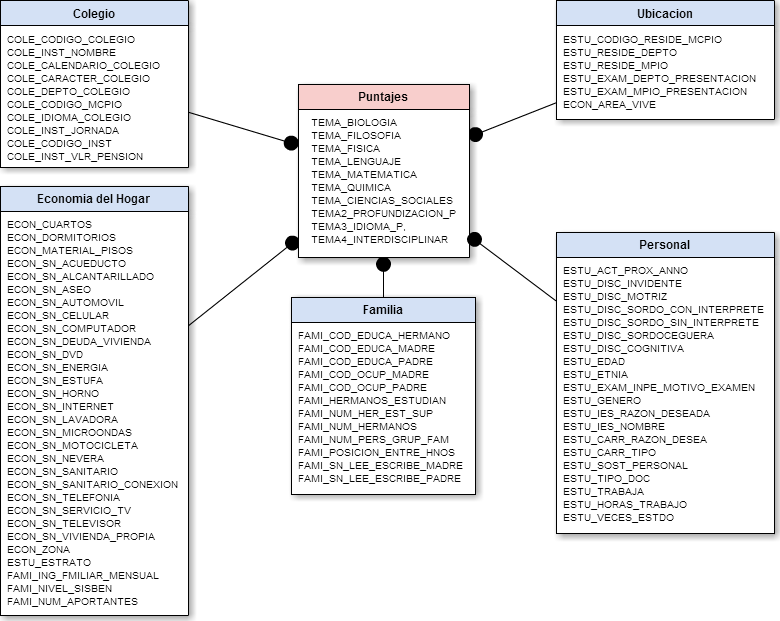
\includegraphics[scale=0.65]{datamart}
\par\end{centering}
\caption{Diseño logico del modelo de almacenamiento de datos.}
\label{fig:figura2}
\end{figure}
En el diseño lógico del modelo dimensional (figura \ref{fig:figura2}) se pueden observar las dimensiones y la tabla de hechos.

Las dimensiones, que contienen los atributos que ayudan a responder las preguntas que se pueden plantear sobre el modelo, constan de la información que define las particularidades de un evaluado. Estas dimensiones son: 
\begin{itemize}
\item \textbf{Colegio}: brinda información sobre el colegio en el que estudia o estudió el evaluado, por ejemplo el carácter, el calendario, la jornada escolar, entre otros.
\item \textbf{Economía del hogar}: brinda información sobre el ambiente económico del evaluado, como por ejemplo las características físicas de su hogar, como el material de los pisos y los sistemas de servicios públicos disponibles en él. Además de informar también sobre los ingresos monetarios y la cantidad de personas en las que deben repartirse estos ingresos.
\item \textbf{Familia}: brinda información sobre las características de la familia del evaluado, como por ejemplo las ocupaciones y niveles educativos de sus padres y hermanos.
\item \textbf{Ubicación}: brinda información sobre la zona geográfica donde vive el evaluado, como el municipio y departamento, y si vive en una zona rural o urbana.
\item \textbf{Personal}: brinda información sobre las características físicas y de personalidad del estudiantes, como su edad, el genero, información sobre discapacidades, las razones que lo llevaron a escoger una carrera, entre otras.
\end{itemize}
Para una mayor información sobre el significado de cada uno de estos atributos y de la forma en cómo se almacenan en las bases de datos, se puede observar el diccionario de datos del ICFES.

En la tabla de hechos, la cual almacena los atributos que contienen la información con la cual se responderá  a las preguntas planteadas al modelo, se pueden observar los registros que indican el puntaje en cada una de las áreas académicas evaluadas. 

Cómo se relacionó en la sección \ref{sec:saber11}, las áreas académicas son 14, 8 de obligatoria presentación para todos los evaluados y 6 áreas electivas de las cuales se debe elegir una. Estas 6 electivas constan de 4 profundizaciones y 2 pruebas interdisciplinares, por eso en los atributos de la tabla hechos se encuentran los atributos  TEMA2_PROFUNDIZACION_P, TEMA4_INTERDISCIPLINAR, estos fueron interpretados con la ayuda de un código que indicaba cual prueba escogió cada evaluado.

Así, con el procesamiento de esta información, que fue recolectada, homogeneizada y almacenada nuevamente, se pudo proceder a trabajar con los distintos algoritmos de clasificación elegidos para evaluar en el trabajo de grado. La descripción del desarrollo de esta etapa de evaluación se encuentra en el siguiente capítulo.
\chapter{Evaluación de Clasificadores}
Después de tener cargado el nuevo almacenamiento de datos con la información homogeneizada, se procedió a evaluar los algoritmos de clasificación para elegir los más confiables para construir la interfaz de consultas, que permita conocer los posibles resultados de un evaluado.

El objetivo de este trabajo de grado era entregar información sobre los posibles resultados de un estudiante en cada una de las áreas académicas evaluadas por la prueba Saber 11\degree. Estas áreas son en total 14, así que para cada una de estas áreas se debió construir un clasificador que predijera con el mayor índice de confianza el resultado a obtener por el evaluado. (En el anexo D se encuentra información sobre como interpretar los resultados de la prueba).
\section{Selección de atributos}
El primer paso para la construcción de estos clasificadores fue filtrar la cantidad de atributos predictores disponibles. Al momento de realizar esta fase se contaba con 78 atributos predictores, varios de estos atributos constaban con una gran cantidad de registros nulos, ya que la frecuencia con la que se almacenó en las bases de datos fue muy baja.

Para la selección de estos atributos a ser filtrados se evaluó primero la cantidad de veces en las que este fue registrado, y utilizando la suite de algoritmos de minera de datos Weka\footnote{\url{http://www.cs.waikato.ac.nz/ml/weka/}} se realizó un filtro de selección de atributos utilizando algoritmos especializados para esta tarea.
\subsection{Selección manual}
La tabla \ref{tab:cuadro15} muestra los atributos que se seleccionaron de manera manual, el criterio para esta primera selección fue que al menos estuvieran presentes en 12 (50\%) de las bases de datos consultadas.

\begin{table}[!Hhtb]
\centering
\begin{tabular}{|p{0.5cm}|p{8cm}|p{1.8cm}|}
\hline
	\rowcolor[gray]{0.9} 
	\textbf{ID} &
	\textbf{Atributo} &
	\textbf{Cantidad}\\
\hline
4 & COLE_CODIGO_MCPIO* & 24 \\ \hline
6 & COLE\_INST\_JORNADA & 24 \\ \hline
7 & COLE\_INST\_VLR\_PENSION & 24 \\ \hline
36 & ESTU\_DISC\_MOTRIZ & 24 \\ \hline
37 & ESTU\_DISC\_SORDO\_CON\_INTERPRETE & 24 \\ \hline
38 & ESTU\_DISC\_SORDO\_SIN\_INTERPRETE & 24 \\ \hline
41 & ESTU\_EDAD & 24 \\ \hline
47 & ESTU\_GENERO & 24 \\ \hline
35 & ESTU\_DISC\_INVIDENTE & 22 \\ \hline
44 & ESTU\_EXAM\_DEPTO\_PRESENTACION & 22 \\ \hline
51 & ESTU\_RESIDE\_DEPTO & 22 \\ \hline
1 & COLE\_CALENDARIO\_COLEGIO & 17 \\ \hline
2 & COLE\_CARACTER\_COLEGIO & 17 \\ \hline
48 & ESTU\_IES\_RAZON\_DESEADA & 17 \\ \hline
49 & ESTU\_CARR\_RAZON\_DESEA & 17 \\ \hline
55 & ESTU\_TRABAJA & 17 \\ \hline
58 & FAMI\_COD\_EDUCA\_MADRE & 17 \\ \hline
59 & FAMI\_COD\_EDUCA\_PADRE & 17 \\ \hline
60 & FAMI\_COD\_OCUP\_MADRE & 17 \\ \hline
61 & FAMI\_COD\_OCUP\_PADRE & 17 \\ \hline
63 & FAMI\_ING\_FMILIAR\_MENSUAL & 17 \\ \hline
68 & FAMI\_NUM\_PERS\_GRUP\_FAM & 17 \\ \hline
3 & COLE\_DEPTO\_COLEGIO & 16 \\ \hline
5 & COLE\_IDIOMA\_COLEGIO & 15 \\ \hline
43 & ESTU\_ETNIA & 15 \\ \hline
46 & ESTU\_EXAM\_MPIO\_PRESENTACION & 15 \\ \hline
52 & ESTU\_RESIDE\_MPIO & 15 \\ \hline
54 & ESTU\_TIPO\_DOC & 14 \\ \hline
\end{tabular}
\caption{Atributos predictores seleccionados de manera manual.}
\label{tab:cuadro15}
\end{table}
\begin{quote}
* Originalmente el atributo registrado 24 veces era COLE_INST_NOMBRE, pero como este tenía alrededor de 12500 opciones, se volvió complicado trabajar con él, por lo tanto se decidió utilizar este para conocer el municipio al que el colegio pertenece y así el atributo COLE_CODIGO_MCPIO se pudo registrar las 24 veces.
\end{quote}
Tras aplicar este primer filtro la cantidad de atributos predictores considerados útiles, se redujo a 28.
Después, usando estos 28 atributos, se procedió a utilizar los algoritmos de selección de atributos predictores disponibles en Weka.
\subsection{Selección automática}
Weka brinda la capacidad de realizar esta selección de atributos utilizando métodos evaluadores que se dividen en 2 tipos: los evaluadores de subconjuntos y los prorrateadores de atributos. El primer tipo se encarga de evaluar cual subconjunto de datos es el mejor para predecir la clase, este utiliza un método de búsqueda del tipo forward o backward. El segundo tipo no evalúa subconjuntos, si no que asigna a cada atributo un valor que indica el nivel de correlación que posee con la clase a predecir, este al contrario de utilizar un método de búsqueda, utiliza un ranker para indicar la importancia de cada atributo.

El primer paso para poder utilizar Weka fue construir los archivos arff\footnote{\url{http://weka.wikispaces.com/ARFF}} estos son los archivos que usa Weka para transmitir la información a los algoritmos. En la primera prueba se construyó un archivo arff con 1000 registros, con los datos obtenidos desde el almacenamiento de datos construido en el capítulo anterior. La idea de realizar esta prueba inicial era determinar los tiempos que demoraba cada posible combinación entre los métodos de evaluación y los métodos de búsqueda que ofrece Weka. Después de realizar esta prueba se optó por la utilización de 6 combinaciones que fueron las que lograron manipular la cantidad de datos presentados, en un tiempo aceptable, teniendo en cuenta que más adelante se ejecutarían pruebas con archivos que contenían hasta 500.000 registros.

La razón para que algunas combinaciones no fueran seleccionadas, fue porque nunca se logró obtener una solución en el tiempo otorgado (20 minutos) o lanzaron error al momento de procesar el archivo. El tiempo de 20 minutos, fue tomado como un límite justificable, ya que de los algoritmos de los cuales si se obtuvo respuesta, no tomaron un tiempo mayor a 3 minutos.

La tabla \ref{tab:cuadro16} muestra las combinaciones seleccionadas.

Como ya se explicó que se construyó un clasificador por cada área evaluada, la selección de atributos también se aplicó a cada una de estas clases a predecir, es decir que por cada área se crearon los archivos arff para ser analizados en los algoritmos.

Los archivos ARFF creados para realizar cada prueba fueron construidos seleccionando de manera aleatoria registros de la base de datos homogeneizada. Además estos archivos fueron creados con distintas cantidades de registros, con el fin de tener una mejor visión sobre el comportamiento de los algoritmos a medida que se aumentaba la cantidad de registros. Estas cantidades fueron 1.000, 10.000, 100.000 y 500.000. Es decir, por cada área evaluada se crearon 4 archivos arff que fueron ejecutados en las 6 combinaciones distintas, dando así 24 evaluaciones a analizar. 

\begin{table}[!Hhtb]
\centering
\begin{tabular}{|p{1cm}|p{6cm}|p{6cm}|}
\hline
	\rowcolor[gray]{0.9}
	\textbf{ID} &
	\textbf{Método de evaluación} &
	\textbf{Método de búsqueda}\\
\hline
1 & CfsSubsetEval\protect\footnotemark & BestFirst\protect\footnotemark \\ \hline
2 & CfsSubsetEval  & GeneticSearch\protect\footnotemark  \\ \hline
3 & CfsSubsetEval  & GreedyStepwise\protect\footnotemark \\ \hline
4 & ClassifierSubsetEval\protect\footnotemark & GeneticSearch \\ \hline
5 & GainRatioAttributeEval\protect\footnotemark & Ranker\protect\footnotemark \\ \hline
6 & InfoGainAttributeEval\protect\footnotemark & Ranker  \\ \hline
\end{tabular}
\caption{Combinaciones utilizadas en Weka para seleccionar atributos predictores.}
\label{tab:cuadro16}
\end{table}
\addtocounter{footnote}{-7}
\footnotetext{\url{http://weka.sourceforge.net/doc.stable/weka/attributeSelection/CfsSubsetEval.html}}
\addtocounter{footnote}{1}
\footnotetext{\url{http://weka.sourceforge.net/doc.stable/weka/attributeSelection/BestFirst.html}}
\addtocounter{footnote}{1}
\footnotetext{\url{http://weka.sourceforge.net/doc.stable/weka/attributeSelection/GeneticSearch.html}}
\addtocounter{footnote}{1}
\footnotetext{\url{http://weka.sourceforge.net/doc.stable/weka/attributeSelection/GreedyStepwise.html}}
\addtocounter{footnote}{1}
\footnotetext{\url{http://weka.sourceforge.net/doc.stable/weka/attributeSelection/ClassifierSubsetEval.html}}
\addtocounter{footnote}{1}
\footnotetext{\url{http://weka.sourceforge.net/doc.stable/weka/attributeSelection/GainRatioAttributeEval.html}}
\addtocounter{footnote}{1}
\footnotetext{\url{http://weka.sourceforge.net/doc.stable/weka/attributeSelection/Ranker.html}}
\addtocounter{footnote}{1}
\footnotetext{\url{http://weka.sourceforge.net/doc.stable/weka/attributeSelection/InfoGainAttributeEval.html}}
\section{Creación de vistas minables}
Posterior a la ejecución de los algoritmos de selección automática, se reevaluó la calidad de los atributos predictores y su capacidad de ser realmente aportantes al momento de predecir el posible puntaje en un área académica. Se decidió que los atributos ESTU_EXAM_MPIO_PRESENTACION y ESTU_EXAM_DEPTO_PRESENTACION no serían tenidos en cuenta para la construcción de los clasificadores, ya que al analizar la base de datos, en más del 90\% de los casos el valor de estos 2 atributos era equivalente al valor de los atributos COLE_CODIGO_MCPIO y COLE_DEPTO_COLEGIO respectivamente, por lo tanto se generaba redundancia en los datos y esto ocasiona que la calidad de las predicciones disminuya. 

También el atributo ESTU_TIPO_DOC que indica el tipo de documento con el que la persona se inscribió, no entregaba información realmente útil. Al analizar la base de datos alrededor del 95\% de los registros se dividían entre ``Tarjeta de Identidad'' o “Cedula de Ciudadanía”, los otros valores posibles no eran comunes. Este atributo se solapa con el atributo ESTU_EDAD, ya que el valor “Tarjeta de Identidad” los tenían los evaluados menores de 18 años y “Cedula de Ciudadanía” los evaluadores mayores de 18 años. Por lo tanto, es claro que conociendo la edad de un evaluado, se puede conocer qué tipo de documento utiliza, así que la edad absorbió este atributo y por eso no fue tenido en cuenta a la hora de construir los clasificadores.

Después de analizar los resultados de la ejecución de los algoritmo de selección de atributos, se procedió a construir las vistas minables que iban a ser procesadas en cada uno de los algoritmos de construcción de clasificadores.

Para la construcción de estas vista minables, se realizó una selección entre los 28 atributos filtrados inicialmente y los atributos que tuvieron una mayor presencia en los resultados de los algoritmos de selección de atributos. En algunas áreas se crearon 2 vistas minables para tener una mejor perspectiva, respecto a distintos comportamientos. No se definió un límite mínimo de selección de los atributos en los resultados de los algoritmos, la cantidad de atributos que compone cada vista minable se decidió teniendo en cuenta el número de veces que fue seleccionado el más frecuente.

Los procesos de minería de datos involucran, además de los algoritmos, el conocimiento que se tenga sobre el problema, en ocasiones algunos atributos pueden no ser relevantes al momento de ejecutar los algoritmos, pero es conocido por las personas involucradas en el proceso, que estos atributos sí determinan un factor importante en el caso de estudio. Teniendo en cuenta este criterio, algunos atributos que tuvieron poca relevancia en los algoritmos de selección, fueron escogidos para ser predictores, ya que se consideró que su significado podría beneficiar la calidad de las predicciones.

La tabla \ref{tab:cuadro31} muestra los atributos procesados en los algoritmos de selección de atributos, para el caso del área de biología, y la frecuencia con la que los algoritmos de selección le dieron importancia. Cabe aclarar que en el caso de los algoritmos de evaluación que utilizan un método de búsqueda “Ranker” siempre aparecieron todos los valores, pero la puntuación asignada a algunos de ellos era de 0.0 por lo tanto estos no se contaron como atributos seleccionados por ese algoritmo.

\begin{table}[!Hhtb]
\centering
\begin{tabular}{|p{1cm}|p{8cm}|p{3cm}|}
\hline
	\rowcolor[gray]{0.9}
	\textbf{ID} &
	\textbf{Atributo} &
	\textbf{\# de veces que se seleccionó}\\
\hline
58    & FAMI_COD_EDUCA_MADRE & 19 \\
\hline
4     & COLE_CODIGO_MCPIO & 17 \\
\hline
41    & ESTU_EDAD & 17 \\
\hline
63    & FAMI_ING_FMILIAR_MENSUAL & 17 \\
\hline
6     & COLE_INST_JORNADA & 16 \\
\hline
52    & ESTU_RESIDE_MPIO & 16 \\
\hline
7     & COLE_INST_VLR_PENSION & 15 \\
\hline
59    & FAMI_COD_EDUCA_PADRE & 15 \\
\hline
60    & FAMI_COD_OCUP_MADRE & 15 \\
\hline
51    & ESTU_RESIDE_DEPTO & 12 \\
\hline
3     & COLE_DEPTO_COLEGIO & 8 \\
\hline
38    & ESTU_DISC_SORDO_SIN_INTERPRETE & 8 \\
\hline
43    & ESTU_ETNIA & 7 \\
\hline
61    & FAMI_COD_OCUP_PADRE & 7 \\
\hline
5     & COLE_IDIOMA_COLEGIO & 6 \\
\hline
47    & ESTU_GENERO & 6 \\
\hline
49    & ESTU_CARR_RAZON_DESEA & 6 \\
\hline
48    & ESTU_IES_RAZON_DESEADA & 5 \\
\hline
36    & ESTU_DISC_MOTRIZ & 4 \\
\hline
37    & ESTU_DISC_SORDO_CON_INTERPRETE & 4 \\
\hline
1     & COLE_CALENDARIO_COLEGIO & 3 \\
\hline
35    & ESTU_DISC_INVIDENTE & 3 \\
\hline
2     & COLE_CARACTER_COLEGIO & 2 \\
\hline
68    & FAMI_NUM_PERS_GRUP_FAM & 2 \\
\hline
55    & ESTU_TRABAJA & 1 \\
\hline
\end{tabular}
\caption{Cantidad de veces que los atributos fueron seleccionados como buenos predictores por los algoritmos de selección de atributos, en el área de biología.}
\label{tab:cuadro31}
\end{table}
En la tabla \ref{tab:cuadro31} se observa los atributos ordenados con base a la relevancia que tuvieron en los algoritmos de selección. Para crear las vistas minables se seleccionaron los de mayor frecuencia.

El criterio aplicado, en el caso de biología, a la selección de los atributos fue que estos se encontraran en al menos 12 de las combinaciones, es decir en el 50\% de estas, 10 atributos cumplieron con este criterio.

Después de analizar estos primeros 10 atributos se pudo notar que existían 2 que indicaban la misma información pero con diferente granularidad, estos eran COLE_DEPTO_COLEGIO y COLE_CODIGO_MCPIO, ambos indican la ubicación del colegio, uno a nivel departamental y el otro a nivel municipal, por lo tanto solo era necesario seleccionar uno de ellos para indicar la ubicación del colegio. Pero como los 2 tenían una frecuencia que cumplía con el criterio, se decidió crear 2 vista minables en donde una tuviera una granularidad de departamento en la ubicación del colegio y la otra una granularidad de municipio en la ubicación del colegio.

Así, siguiendo una lógica similar a la aplicada al área de biología, se crearon las vistas minables de las demás áreas académicas.

En las 14 áreas académicas se intentó seguir las mismas reglas de manera general, pero en algunas áreas como por ejemplo medio ambiente, eran pocos los atributos que cumplían con estar seleccionado en al menos 12 combinaciones, en el caso de medio ambiente, solo 3 atributos cumplían esto.
 
También para el caso de algunos atributos, como FAMI_COD_OCUP_PADRE, no tuvieron buena frecuencia de selección, pero FAMI_COD_OCUP_MADRE si lo hizo, teniendo en cuenta que estos indican la misma información de los padres, en algunas vistas minables se agregó la ocupación del padre como atributo a pesar de que su frecuencia de selección no fuera alta.

La tabla \ref{tab:cuadro32} muestra las vistas minables creadas para cada una de las áreas académicas.

\begin{table}[!Hhtb]
\centering
\begin{tabular}{|p{3.5cm}|p{7cm}|}
\hline
	\rowcolor[gray]{0.9} 
	\multicolumn{2}{|c|}{
	\textbf{Vistas minables}}\\
\hline
	\rowcolor[gray]{0.5}
	Nombre & Atributos\\
\hline
Biologia9 & 6, 7, 41, 51, 58, 59, 60, 61, 63 \\
\hline
Biologia10 & 4, 6, 7, 41, 52, 58, 59, 60, 61, 63 \\
\hline
Filosofia7 & 1, 4, 7, 41, 52, 58, 59 \\
\hline
Fisica11 & 1, 4, 7, 41, 47, 52, 58, 59, 60, 61, 63 \\
\hline
Fisica112 & 1, 6, 7, 41, 47, 52, 58, 59, 60, 61, 63 \\
\hline
Ingles11 & 4, 5, 6, 7, 41, 52, 58, 59, 60, 61, 63 \\
\hline
Lenguaje10 & 4, 7, 41, 43, 52, 58, 59, 60, 61, 63 \\
\hline
Lenguaje102 & 4, 6, 7, 41, 43, 58, 59, 60, 61, 63 \\
\hline
Matematica10 & 4, 6, 7, 41, 47, 52, 58, 59, 60, 61 \\
\hline
Matematica102 & 1, 3, 6, 7, 41, 47, 58, 59, 60, 61 \\
\hline
MedioAmbiente5 & 2, 4, 52, 58, 60 \\
\hline
MedioAmbiente7 & 2, 4, 52, 58, 59, 60, 61 \\
\hline
ProBiologia6 & 1, 4, 7, 58, 60, 63 \\
\hline
ProBiologia8 & 1, 4, 7, 58, 59, 60, 61, 63 \\
\hline
ProLenguaje7 & 2, 4, 7, 41, 58, 60, 63 \\
\hline
ProLenguaje9 & 2, 4, 7, 41, 58, 59, 60, 61, 63 \\
\hline
ProMatematica7 & 4, 6, 7, 41, 58, 60, 63 \\
\hline
ProMatematica9 & 4, 6, 7, 41, 58, 59, 60, 61, 63 \\
\hline
ProSociales7 & 1, 4, 7, 41, 58, 60, 63 \\
\hline
ProSociales9 & 1, 4, 7, 41, 58, 59, 60, 61, 63 \\
\hline
Quimica10 & 4, 6, 7, 41, 52, 58, 59, 60, 61, 63 \\
\hline
Sociales7 & 4, 7, 41, 52, 58, 60, 63  \\
\hline
Sociales9 & 4, 7, 41, 52, 58, 59, 60, 61, 63  \\
\hline
Violencia11 & 4, 6, 7, 41, 52, 55, 58, 59, 60, 61, 63 \\
\hline
\end{tabular}
\caption{Lista de las vistas minables creadas.}
\label{tab:cuadro32}
\end{table}
Teniendo lista la estructura para construir las vistas minables, se procedió a la carga de estas. Cada vista minable se creó con 1.000, 10.000 y 100.000 registros.

Las vistas minables se cargaron utilizando el lenguaje de programación Python. Se utilizó el generador de números aleatorios para seleccionar los registros en la base de datos de manera que se aseguró que no existía ninguna correlación entre los registros cargados. También se aseguró que estos registros fueran cargados sin ninguno de sus atributos con valor nulo, esto se hizo con el fin de que los algoritmos de clasificación tuvieran una mejor confiabilidad.

En el caso de las profundizaciones, en donde la cantidad de registros es menor, ya que la presentación de estas pruebas es opcional, no se pudieron crear vistas minables de 100.000 registros, porque fue difícil lograr que todos los atributos coincidieran en no ser nulos, por eso en las profundizaciones los grupos fueron de 1.000, 10.000 y 50.000.

Con las vistas minables cargadas, se procedió a la evaluación de estos en los algoritmos de construcción de clasificadores.
\section{Construcción de clasificadores}
Utilizando Weka, se procedió a generar distintos clasificadores, con base en los anteriores trabajos revisados y que sirvieron de apoyo para este, los algoritmos seleccionados para evaluar las vistas minables fueron: generador de árboles de decisión C4.5\cite{key-170}, K vecinos más cercanos\cite{key-180}, Naive Bayes\cite{key-190} y red neuronal RBF (Radial Basis Function)\cite{key-200}.

Weka ofrece la posibilidad de ejecutar cada uno de estos algoritmos con una colección de datos de entrenamiento y evaluar su nivel de confianza con un archivo de evaluación.

Los archivos de entrenamiento fueron aquellos que se crearon siguiendo la estructura de las vistas minables presentadas en la anterior sección. En Weka es posible dividir estos archivos, para que un porcentaje sea de entrenamiento y el otro porcentaje sea de evaluación. Pero en este trabajo se decidió crear los archivos de evaluación a partir de un conjunto de datos completamente nuevo y desconocido para el conjunto de datos de entrenamiento, esto se logró utilizando los resultados de la prueba en el año 2012. 

Como se había explicado inicialmente, en el momento de iniciar este trabajo las bases de datos disponibles eran las de los años 2000 hasta 2011, pero en el momento de iniciar la creación de los clasificadores, la base de datos del año 2012 estaba disponible para su descarga y se pudo utilizar como un conjunto de datos desconocido para el conjunto de datos inicial.

Para cada vista minable se creó un archivo que tenía la misma estructura pero que se cargaba con registros de la base de datos de 2012, estos archivos de evaluación se crearon con una cantidad de 1000 registros. Es decir que por cada clasificador creado, se evaluaba su precisión con 1000 registros de los cuales se conocía la clase, pero al clasificador se le presentaba como desconocida, para que la predijera.

La precisión se calculó de manera lineal, por ejemplo si en los archivos de evaluación se tenía un registro con calificación, en alguna de las áreas académicas, de F (entre 50 y 60 puntos) y el clasificador lo asignaba en la clase F, entonces se entendía como un 100\% de éxito en la predicción. En el caso de que el clasificador lo asignara en la clase E, se entendía como un 90\% de éxito, ya que se trabajó con 10 niveles y en este caso el error de un nivel es un 10\% menos de confianza en la precisión. Así, si por ejemplo, se hubiera predicho en la clase B el nivel de confianza era de 60\%.

Con estas evaluaciones para visualizar el nivel de confianza que ofrecía cada clasificador, fue que se tomó la decisión de cuales clasificadores iban a ser utilizados en la construcción de la interfaz de consultas.

A continuación se presentan los resultados de cada algoritmo construido con cada una de las vistas minables definidas para predecir cada área académica.
\subsection{Generador de árboles de decisión C4.5}
El algoritmo de árboles de clasificación C4.5 se encuentra implementado en Weka en la librería J48\footnote{\url{http://weka.sourceforge.net/doc.stable/weka/classifiers/trees/J48.html}}.

Un árbol de decisión es un conjunto de condiciones organizadas en una estructura jerárquica. De tal manera que la decisión final se puede tomar siguiendo las condiciones desde la raíz hasta alguna de las hojas.

El problema de la construcción de un árbol puede ser explicado de una manera recursiva, Primero se selecciona un atributo para ser ubicado en la raíz del árbol, y se crea una rama por cada posible valor que puede tomar este atributo. Esto divide el conjunto de datos de entrenamiento en distintas secciones con cada valor del nodo raíz. Y el proceso se repite de manera recursiva por cada una de las nuevas ramas, usando las instancias que están presentes en cada nuevo nodo. La condición de parada es cuando todas las instancias en un nodo tiene la misma clasificación\cite{key-210}.
\begin{figure}[H]
\begin{centering}
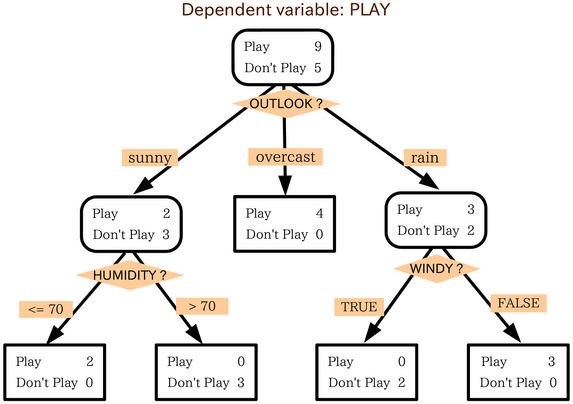
\includegraphics[scale=0.6]{c45}
\par\end{centering}
\caption{Representación gráfica de un árbol de decisión.}
\end{figure}
El algoritmo, se entrenó y evaluó con cada una de las vistas minables de las áreas académicas, los resultados obtenidos, en cada uno de los clasificadores, se muestran en la tabla \ref{tab:cuadro33}.\\

\begin{longtable}{|p{3cm}|p{3cm}|p{2cm}|p{2cm}|p{2cm}|p{2cm}|}
%\centering
%\begin{tabular}{|p{3cm}|p{3cm}|p{2cm}|p{2cm}|p{2cm}|p{2cm}|}
\hline
	\rowcolor[gray]{0.5} 
	\multicolumn{2}{|c|}{Vista minable} &
	\multicolumn{4}{|c|}{Porcentaje de éxito de las instancias clasificadas}\\
	\hline
	\rowcolor[gray]{0.9} 
	Nombre & \# de instancias & 100\% & 90\% & 80\% & 70\%\\
	\hline
	\endhead
	\hline
	\multicolumn{6}{r}{\textit{Continua en la siguiente pagina.}} \\
	\endfoot
	\endlastfoot
	\multirow{3}[5]{*}{Biologia9} & 1000  & 445   & 481   & 67    & 7\\
\cline{2-6}      & 10000 & 445   & 481   & 67    & 7 \\
\cline{2-6}      & 100000 & 453   & 481   & 59    & 7 \\
\hline
\multirow{3}[6]{*}{Biologia10} & 1000  & 496   & 434   & 65    & 4 \\
\cline{2-6}      & 10000 & 496   & 434   & 65    & 4 \\
\cline{2-6}      & 100000 & 499   & 433   & 63    & 4 \\
\hline
\multirow{3}[6]{*}{Filosofia7} & 1000  & 399   & 490   & 93    & 17 \\
\cline{2-6}      & 10000 & 399   & 490   & 93    & 17 \\
\cline{2-6}      & 100000 & 399   & 490   & 93    & 17 \\
\hline
\multirow{3}[6]{*}{Fisica11} & 1000  & 540   & 400   & 56    & 2 \\
\cline{2-6}      & 10000 & 540   & 400   & 56    & 2 \\
\cline{2-6}      & 100000 & 540   & 400   & 56    & 2 \\
\hline
\multirow{3}[6]{*}{Fisica112} & 1000  & 517   & 419   & 60    & 4 \\
\cline{2-6}      & 10000 & 517   & 419   & 60    & 4 \\
\cline{2-6}      & 100000 & 517   & 419   & 60    & 4 \\
\hline
\multirow{2}[4]{*}{Ingles11} & 1000  & 428   & 417   & 80    & 40 \\
\cline{2-6}      & 10000 & 519   & 329   & 80    & 12 \\
\hline
\multirow{3}[6]{*}{Lenguaje10} & 1000  & 548   & 406   & 44    & 1 \\
\cline{2-6}      & 10000 & 548   & 406   & 44    & 1 \\
\cline{2-6}      & 100000 & 509   & 432   & 56    & 2 \\
\hline
\multirow{3}[6]{*}{Lenguaje102} & 1000  & 580   & 392   & 25    & 3 \\
\cline{2-6}      & 10000 & 580   & 392   & 25    & 3 \\
\cline{2-6}      & 100000 & 580   & 392   & 25    & 3 \\
\hline
\multirow{3}[6]{*}{Matematica10} & 1000  & 356   & 519   & 97    & 18 \\
\cline{2-6}      & 10000 & 356   & 519   & 97    & 18 \\
\cline{2-6}      & 100000 & 356   & 519   & 97    & 18 \\
\hline
\multirow{3}[6]{*}{Matematica102} & 1000  & 346   & 508   & 108   & 25 \\
\cline{2-6}      & 10000 & 346   & 508   & 108   & 25 \\
\cline{2-6}      & 100000 & 346   & 508   & 108   & 25 \\
\hline
\multirow{3}[6]{*}{MedioAmbiente5} & 1000  & 0     & 847   & 148   & 0 \\
\cline{2-6}      & 10000 & 0     & 847   & 148   & 0 \\
\cline{2-6}      & 100000 & 0     & 847   & 148   & 0 \\
\hline
\multirow{3}[6]{*}{MedioAmbiente7} & 1000  & 4     & 851   & 144   & 0 \\
\cline{2-6}      & 10000 & 4     & 851   & 144   & 0 \\
\cline{2-6}      & 100000 & 4     & 851   & 144   & 0 \\
\hline
\multirow{3}[6]{*}{ProBiologia6} & 1000  & 285   & 426   & 258   & 25 \\
\cline{2-6}      & 10000 & 263   & 417   & 279   & 34 \\
\cline{2-6}      & 50000 & 263   & 417   & 279   & 34 \\
\hline
\multirow{3}[6]{*}{ProBiologia8} & 1000  & 314   & 396   & 242   & 40 \\
\cline{2-6}      & 10000 & 314   & 396   & 242   & 40 \\
\cline{2-6}      & 50000 & 280   & 404   & 254   & 53 \\
\hline
\multirow{3}[6]{*}{ProLenguaje7} & 1000  & 207   & 559   & 223   & 10 \\
\cline{2-6}      & 10000 & 207   & 559   & 223   & 10 \\
\cline{2-6}      & 50000 & 207   & 559   & 223   & 10 \\
\hline
\multirow{3}[6]{*}{ProLenguaje9} & 1000  & 221   & 545   & 221   & 8 \\
\cline{2-6}      & 10000 & 221   & 545   & 221   & 8 \\
\cline{2-6}      & 50000 & 221   & 545   & 221   & 8 \\
\hline
\multirow{3}[6]{*}{ProMatematica7} & 1000  & 176   & 697   & 87    & 31 \\
\cline{2-6}      & 10000 & 176   & 697   & 87    & 31 \\
\cline{2-6}      & 50000 & 232   & 653   & 78    & 28 \\
\hline
\multirow{3}[6]{*}{ProMatematica9} & 1000  & 157   & 686   & 101   & 48 \\
\cline{2-6}      & 10000 & 157   & 686   & 101   & 48 \\
\cline{2-6}      & 50000 & 160   & 684   & 101   & 47 \\
\hline
\multirow{3}[6]{*}{ProSociales7} & 1000  & 184   & 600   & 205   & 9 \\
\cline{2-6}      & 10000 & 184   & 600   & 205   & 9 \\
\cline{2-6}      & 50000 & 213   & 517   & 224   & 38 \\
\hline
\multirow{3}[6]{*}{ProSociales9} & 1000  & 174   & 605   & 211   & 7 \\
\cline{2-6}      & 10000 & 174   & 605   & 211   & 7 \\
\cline{2-6}      & 50000 & 188   & 554   & 220   & 33 \\
\hline
\multirow{3}[6]{*}{Quimica10} & 1000  & 640   & 328   & 30    & 2 \\
\cline{2-6}      & 10000 & 640   & 328   & 30    & 2 \\
\cline{2-6}      & 100000 & 640   & 328   & 30    & 2 \\
\hline
\multirow{3}[6]{*}{Sociales7} & 1000  & 474   & 439   & 81    & 5 \\
\cline{2-6}      & 10000 & 474   & 439   & 81    & 5 \\
\cline{2-6}      & 100000 & 474   & 439   & 81    & 5 \\
\hline
\multirow{3}[6]{*}{Sociales9} & 1000  & 466   & 457   & 70    & 4 \\
\cline{2-6}      & 10000 & 466   & 457   & 70    & 4 \\
\cline{2-6}      & 100000 & 466   & 457   & 70    & 4 \\
\hline
\multirow{3}[6]{*}{Violencia11} & 1000  & 457   & 424   & 104   & 14 \\
\cline{2-6}      & 10000 & 457   & 424   & 104   & 14 \\
\cline{2-6}      & 100000 & 457   & 424   & 104   & 14 \\
\hline
%\end{tabular}
\caption{Resultados de la construcción y evaluación de las vistas minables usando el algoritmo C4.5.}
\label{tab:cuadro33}
\end{longtable}
En la tabla \ref{tab:cuadro33} se puede observar que todos los clasificadores, creados con cada una de las vistas minables, tuvieron más del 70\% de éxito en al menos el 90\% de las instancias presentadas en los archivos de evaluación.

También se resalta, que en varias de las vistas minables, la cantidad de registros con los que se entrenó el clasificador, no causaron un diferencia en la precisión de este.

Los clasificadores obtenidos usando el algoritmo C4.5 tuvieron un grado de confianza considerablemente positivo, pero la estabilidad presentada al momento de cambiar la cantidad de registro, causó desconfianza sobre la calidad de la precisión. 
Al analizar los arboles generados por los algoritmos, se encontró que los arboles solo se generaban con un nodo, que inmediatamente clasificaba la clase a la que pertenecía la instancia. Esta clase era la que más veces se encontraba en el archivo de evaluación.

Por ejemplo, el archivo de entrenamiento Biologia9 con 1.000 registros, contenía 579 instancias en la clase E, 228 en la clase F y 158 en la clase D. Al procesar el algoritmo con este archivo, el árbol generado, solo tenía un nodo donde todas las instancias de evaluación, se clasificaban en la clase E. Por lo tanto, estos resultados, solo asignan una predicción basándose en la clase mayoritariamente encontrada en las instancias de entrenamiento, así que su confianza no es realmente significativa.\\
\subsection{K vecinos más cercanos}
El algoritmo de los K vecinos más cercanos se encuentra implementado en Weka en la librería IBK\footnote{\url{http://weka.sourceforge.net/doc.stable/weka/classifiers/lazy/IBk.html}}.

La regla del vecino más cercano es simple, este asigna a la instancia que se quiere clasificar, la clase del ejemplo más próximo utilizando una función de distancia. Esta función usualmente es la función de distancia Euclidiana, aunque una alternativa también frecuentemente usada es la función de distancia Manhattan.

El problema con esta sencilla manera de clasificar las instancias, es que toma mucho tiempo comparar, cada una de las instancias de entrenamiento con la instancia a clasificar, para determinar cuál es la más cercana. La manera de reducir el tiempo que toma esta comparación es representando los datos de entrenamiento como un árbol, este árbol es llamado un kD-tree\cite{key-220}, porque almacena un grupo de puntos en un espacio k-dimensional. Siendo k el número de atributos de las instancias.

El uso de los kD-tree ha ayudado a solucionar el problema de la comparación uno por uno, ya que el árbol divide el espacio en dimensiones que agrupan instancias con atributos similares, así cada evaluación no debe compararse contra cada instancia, sino que se compara contra las dimensiones, y se asigna a la clase de la dimension con la que tuvo una mayor similitud\cite{key-210}.

Se procedió a ejecutar el algoritmo con 2 distintas configuraciones para obtener los clasificadores de cada vista minable. Una configuración utilizó un valor de K=1 el cual indicaba la cantidad de vecinos mas cercanos que se iban a buscar para asignar un valor a la instancia evaluada. La otra configuración usó este valor en K=2. Los resultados de la configuración con K=1 se muestra en la tabla \ref{tab:cuadro34} y los resultados con K=2 en la tabla \ref{tab:cuadro35}.\\

\begin{longtable}{|p{3cm}|p{3cm}|p{2cm}|p{2cm}|p{2cm}|p{2cm}|}
%\centering
%\begin{tabular}{|p{3cm}|p{3cm}|p{2cm}|p{2cm}|p{2cm}|p{2cm}|}
\hline
	\rowcolor[gray]{0.5} 
	\multicolumn{2}{|c|}{Vista minable} &
	\multicolumn{4}{|c|}{Porcentaje de éxito de las instancias clasificadas}\\
	\hline
	\rowcolor[gray]{0.9} 
	Nombre & \# de instancias & 100\% & 90\% & 80\% & 70\%\\
	\hline
	\endhead
	\hline
	\multicolumn{6}{r}{\textit{Continua en la siguiente pagina.}} \\
	\endfoot
	\endlastfoot
\multirow{3}[5]{*}{Biologia9} & 1000  & 345   & 495   & 143   & 16 \\
\cline{2-6}      & 10000 & 387   & 469   & 129   & 12 \\
\cline{2-6}      & 100000 & 388   & 476   & 115   & 17 \\
\hline
\multirow{3}[6]{*}{Biologia10} & 1000  & 416   & 469   & 99    & 14 \\
\cline{2-6}      & 10000 & 447   & 447   & 95    & 9 \\
\cline{2-6}      & 100000 & 442   & 453   & 96    & 8 \\
\hline
\multirow{3}[6]{*}{Filosofia7} & 1000  & 369   & 470   & 131   & 27 \\
\cline{2-6}      & 10000 & 362   & 482   & 125   & 29 \\
\cline{2-6}      & 100000 & 359   & 487   & 130   & 20 \\
\hline
\multirow{3}[6]{*}{Fisica11} & 1000  & 424   & 456   & 109   & 10 \\
\cline{2-6}      & 10000 & 427   & 446   & 111   & 14 \\
\cline{2-6}      & 100000 & 416   & 473   & 100   & 10 \\
\hline
\multirow{3}[6]{*}{Fisica112} & 1000  & 394   & 470   & 115   & 19 \\
\cline{2-6}      & 10000 & 413   & 454   & 118   & 12 \\
\cline{2-6}      & 100000 & 449   & 445   & 92    & 13 \\
\hline
\multirow{2}[4]{*}{Ingles11} & 1000  & 192   & 278   & 200   & 194 \\
\cline{2-6}      & 10000 & 204   & 267   & 202   & 162 \\
\hline
\multirow{3}[6]{*}{Lenguaje10} & 1000  & 412   & 474   & 106   & 7 \\
\cline{2-6}      & 10000 & 452   & 457   & 83    & 7 \\
\cline{2-6}      & 100000 & 457   & 451   & 84    & 7 \\
\hline
\multirow{3}[6]{*}{Lenguaje102} & 1000  & 417   & 448   & 115   & 17 \\
\cline{2-6}      & 10000 & 374   & 476   & 124   & 22 \\
\cline{2-6}      & 100000 & 395   & 470   & 110   & 24 \\
\hline
\multirow{3}[6]{*}{Matematica10} & 1000  & 337   & 470   & 144   & 37 \\
\cline{2-6}      & 10000 & 353   & 454   & 144   & 35 \\
\cline{2-6}      & 100000 & 332   & 497   & 125   & 35 \\
\hline
\multirow{3}[6]{*}{Matematica102} & 1000  & 282   & 420   & 215   & 59 \\
\cline{2-6}      & 10000 & 280   & 445   & 201   & 54 \\
\cline{2-6}      & 100000 & 296   & 421   & 199   & 63 \\
\hline
\multirow{3}[6]{*}{MedioAmbiente5} & 1000  & 237   & 656   & 101   & 0 \\
\cline{2-6}      & 10000 & 222   & 670   & 101   & 0 \\
\cline{2-6}      & 100000 & 196   & 692   & 105   & 0 \\
\hline
\multirow{3}[6]{*}{MedioAmbiente7} & 1000  & 285   & 626   & 85    & 0 \\
\cline{2-6}      & 10000 & 211   & 673   & 115   & 0 \\
\cline{2-6}      & 100000 & 229   & 671   & 98    & 0 \\
\hline
\multirow{3}[6]{*}{ProBiologia6} & 1000  & 212   & 383   & 301   & 89 \\
\cline{2-6}      & 10000 & 211   & 414   & 279   & 84 \\
\cline{2-6}      & 50000 & 207   & 408   & 288   & 82 \\
\hline
\multirow{3}[6]{*}{ProBiologia8} & 1000  & 231   & 374   & 297   & 75 \\
\cline{2-6}      & 10000 & 238   & 375   & 274   & 91 \\
\cline{2-6}      & 50000 & 233   & 381   & 259   & 106 \\
\hline
\multirow{3}[6]{*}{ProLenguaje7} & 1000  & 245   & 500   & 217   & 31 \\
\cline{2-6}      & 10000 & 252   & 494   & 226   & 20 \\
\cline{2-6}      & 50000 & 219   & 517   & 228   & 31 \\
\hline
\multirow{3}[6]{*}{ProLenguaje9} & 1000  & 235   & 498   & 224   & 35 \\
\cline{2-6}      & 10000 & 226   & 522   & 209   & 37 \\
\cline{2-6}      & 50000 & 227   & 502   & 225   & 38 \\
\hline
\multirow{3}[6]{*}{ProMatematica7} & 1000  & 358   & 468   & 121   & 25 \\
\cline{2-6}      & 10000 & 332   & 474   & 132   & 34 \\
\cline{2-6}      & 50000 & 314   & 521   & 114   & 34 \\
\hline
\multirow{3}[6]{*}{ProMatematica9} & 1000  & 322   & 462   & 158   & 40 \\
\cline{2-6}      & 10000 & 316   & 478   & 144   & 33 \\
\cline{2-6}      & 50000 & 301   & 504   & 132   & 41 \\
\hline
ProSociales7 & 1000  & 227   & 513   & 216   & 38 \\
\multirow{2}[6]{*}{ProSociales7}      & 10000 & 244   & 486   & 229   & 37 \\
\cline{2-6}      & 50000 & 235   & 485   & 223   & 49 \\
\hline
\multirow{3}[6]{*}{ProSociales9} & 1000  & 278   & 476   & 190   & 38 \\
\cline{2-6}      & 10000 & 231   & 500   & 234   & 25 \\
\cline{2-6}      & 50000 & 217   & 513   & 228   & 31 \\
\hline
\multirow{3}[6]{*}{Quimica10} & 1000  & 488   & 426   & 73    & 13 \\
\cline{2-6}      & 10000 & 534   & 405   & 53    & 8 \\
\cline{2-6}      & 100000 & 499   & 430   & 59    & 12 \\
\hline
\multirow{3}[6]{*}{Sociales7} & 1000  & 397   & 475   & 119   & 8 \\
\cline{2-6}      & 10000 & 392   & 483   & 115   & 10 \\
\cline{2-6}      & 100000 & 418   & 438   & 132   & 11 \\
\hline
\multirow{3}[6]{*}{Sociales9} & 1000  & 368   & 475   & 137   & 18 \\
\cline{2-6}      & 10000 & 418   & 446   & 121   & 12 \\
\cline{2-6}      & 100000 & 386   & 493   & 106   & 13 \\
\hline
\multirow{3}[6]{*}{Violencia11} & 1000  & 277   & 459   & 195   & 47 \\
\cline{2-6}      & 10000 & 305   & 470   & 170   & 45 \\
\cline{2-6}      & 100000 & 323   & 464   & 167   & 34 \\
\hline
%\end{tabular}
\caption{Resultados de la construcción y evaluación de las vistas minables usando el algoritmo de los K vecinos más cercanos, con un valor de k=1.}
\label{tab:cuadro34}
\end{longtable}

\begin{longtable}{|p{3cm}|p{3cm}|p{2cm}|p{2cm}|p{2cm}|p{2cm}|}
%\centering
%\begin{tabular}{|p{3cm}|p{3cm}|p{2cm}|p{2cm}|p{2cm}|p{2cm}|}
\hline
	\rowcolor[gray]{0.5} 
	\multicolumn{2}{|c|}{Vista minable} &
	\multicolumn{4}{|c|}{Porcentaje de éxito de las instancias clasificadas}\\
	\hline
	\rowcolor[gray]{0.9} 
	Nombre & \# de instancias & 100\% & 90\% & 80\% & 70\%\\
	\hline
	\endhead
	\hline
	\multicolumn{6}{r}{\textit{Continua en la siguiente pagina.}} \\
	\endfoot
	\endlastfoot
\multirow{3}[5]{*}{Biologia9} & 1000  & 350   & 483   & 146   & 21 \\
\cline{2-6}      & 10000 & 410   & 455   & 118   & 15 \\
\cline{2-6}      & 100000 & 387   & 481   & 113   & 15 \\
\hline
\multirow{3}[6]{*}{Biologia10} & 1000  & 418   & 467   & 100   & 13 \\
\cline{2-6}      & 10000 & 453   & 452   & 85    & 8 \\
\cline{2-6}      & 100000 & 438   & 473   & 79    & 10 \\
\hline
\multirow{2}[6]{*}{Filosofia7} & 1000  & 386   & 484   & 114   & 15 \\
\cline{2-6}      & 10000 & 398   & 473   & 108   & 19 \\
Filosofia7      & 100000 & 380   & 486   & 114   & 16 \\
\hline
\multirow{3}[6]{*}{Fisica11} & 1000  & 437   & 450   & 101   & 9 \\
\cline{2-6}      & 10000 & 452   & 438   & 91    & 16 \\
\cline{2-6}      & 100000 & 431   & 469   & 88    & 10 \\
\hline
\multirow{3}[6]{*}{Fisica112} & 1000  & 429   & 443   & 111   & 14 \\
\cline{2-6}      & 10000 & 435   & 433   & 123   & 6 \\
\cline{2-6}      & 100000 & 456   & 448   & 82    & 13 \\
\hline
\multirow{2}[4]{*}{Ingles11} & 1000  & 383   & 417   & 120   & 43 \\
\cline{2-6}      & 10000 & 534   & 322   & 71    & 16 \\
\hline
\multirow{3}[6]{*}{Lenguaje10} & 1000  & 421   & 481   & 92    & 5 \\
\cline{2-6}      & 10000 & 462   & 450   & 81    & 6 \\
\cline{2-6}      & 100000 & 452   & 456   & 85    & 6 \\
\hline
\multirow{3}[6]{*}{Lenguaje102} & 1000  & 413   & 448   & 114   & 19 \\
\cline{2-6}      & 10000 & 378   & 476   & 114   & 27 \\
\cline{2-6}      & 100000 & 399   & 481   & 98    & 20 \\
\hline
\multirow{3}[6]{*}{Matematica10} & 1000  & 326   & 460   & 159   & 40 \\
\cline{2-6}      & 10000 & 345   & 451   & 159   & 31 \\
\cline{2-6}      & 100000 & 329   & 500   & 125   & 34 \\
\hline
\multirow{3}[6]{*}{Matematica102} & 1000  & 271   & 439   & 211   & 51 \\
\cline{2-6}      & 10000 & 278   & 446   & 196   & 61 \\
\cline{2-6}      & 100000 & 301   & 428   & 194   & 54 \\
\hline
\multirow{3}[6]{*}{MedioAmbiente5} & 1000  & 198   & 689   & 108   & 0 \\
\cline{2-6}      & 10000 & 176   & 706   & 112   & 0 \\
\cline{2-6}      & 100000 & 178   & 708   & 107   & 0 \\
\hline
\multirow{3}[6]{*}{MedioAmbiente7} & 1000  & 258   & 652   & 88    & 0 \\
\cline{2-6}      & 10000 & 178   & 702   & 119   & 0 \\
\cline{2-6}      & 100000 & 195   & 700   & 103   & 0 \\
\hline
\multirow{3}[6]{*}{ProBiologia6} & 1000  & 229   & 393   & 292   & 73 \\
\cline{2-6}      & 10000 & 229   & 414   & 275   & 72 \\
\cline{2-6}      & 50000 & 214   & 416   & 278   & 81 \\
\hline
ProBiologia8 & 1000  & 268   & 369   & 284   & 65 \\
\multirow{2}[6]{*}{ProBiologia8} & 10000 & 247   & 392   & 270   & 75 \\
\cline{2-6}      & 50000 & 241   & 388   & 258   & 92 \\
\hline
\multirow{3}[6]{*}{ProLenguaje7} & 1000  & 271   & 517   & 192   & 15 \\
\cline{2-6}      & 10000 & 259   & 520   & 202   & 16 \\
\cline{2-6}      & 50000 & 223   & 536   & 214   & 24 \\
\hline
\multirow{3}[6]{*}{ProLenguaje9} & 1000  & 280   & 516   & 189   & 9 \\
\cline{2-6}      & 10000 & 241   & 539   & 193   & 21 \\
\cline{2-6}      & 50000 & 231   & 523   & 215   & 24 \\
\hline
\multirow{3}[6]{*}{ProMatematica7} & 1000  & 408   & 466   & 76    & 19 \\
\cline{2-6}      & 10000 & 359   & 491   & 107   & 25 \\
\cline{2-6}      & 50000 & 345   & 514   & 95    & 30 \\
\hline
\multirow{3}[6]{*}{ProMatematica9} & 1000  & 353   & 466   & 122   & 37 \\
\cline{2-6}      & 10000 & 342   & 490   & 119   & 30 \\
\cline{2-6}      & 50000 & 310   & 514   & 115   & 35 \\
\hline
\multirow{3}[6]{*}{ProSociales7} & 1000  & 256   & 535   & 180   & 22 \\
\cline{2-6}      & 10000 & 254   & 519   & 196   & 25 \\
\cline{2-6}      & 50000 & 225   & 498   & 222   & 46 \\
\hline
\multirow{3}[6]{*}{ProSociales9} & 1000  & 316   & 509   & 138   & 19 \\
\cline{2-6}      & 10000 & 249   & 535   & 194   & 15 \\
\cline{2-6}      & 50000 & 221   & 525   & 213   & 29 \\
\hline
\multirow{3}[6]{*}{Quimica10} & 1000  & 496   & 419   & 74    & 10 \\
\cline{2-6}      & 10000 & 533   & 398   & 63    & 6 \\
\cline{2-6}      & 100000 & 496   & 428   & 63    & 13 \\
\hline
\multirow{3}[6]{*}{Sociales7} & 1000  & 398   & 475   & 115   & 10 \\
\cline{2-6}      & 10000 & 390   & 484   & 116   & 10 \\
\cline{2-6}      & 100000 & 420   & 446   & 119   & 14 \\
\hline
\multirow{3}[6]{*}{Sociales9} & 1000  & 354   & 484   & 144   & 16 \\
\cline{2-6}      & 10000 & 408   & 464   & 109   & 15 \\
\cline{2-6}      & 100000 & 381   & 494   & 109   & 14 \\
\hline
\multirow{2}[6]{*}{Violencia11} & 1000  & 308   & 462   & 176   & 40 \\
\cline{2-6}      & 10000 & 314   & 477   & 157   & 46 \\
Violencia11      & 100000 & 322   & 475   & 166   & 28 \\
\hline
%\end{tabular}
\caption{Resultados de la construcción y evaluación de las vistas minables usando el algoritmo de los K vecinos más cercanos, con un valor de k=2.}
\label{tab:cuadro35}
\end{longtable}
Cómo en el caso del algoritmo C4.5, alrededor del 90\% de las instancias, en todos los clasificadores construidos, fueron predichas con al menos el 80\% de éxito. Pero a diferencia del algoritmo C4.5 en este sí se notó variaciones al momento de aumentar la cantidad de registros en las vistas minables. Aunque no se pudo encontrar un patrón de comportamiento, al momento de modificar estas cantidades, ya que en algunos casos esto ayudo a mejorar la precisión de las predicciones y en otros casos la disminuyo.

Tampoco se observa una diferencia significativa entre la configuración con k=1 y la de k=2. En términos generales, ambas se comportaron de manera muy similar en las predicciones realizadas.

Los clasificadores creados con este algoritmo generaron predicciones las cuales tienen un nivel de confianza significativo.
\subsection{Naive Bayes}
El algoritmo Naive Bayes se encuentra implementado en Weka en la librería del mismo nombre\footnote{\url{http://weka.sourceforge.net/doc.stable/weka/classifiers/bayes/NaiveBayes.html}}.

Los métodos bayesianos combaten uno de los problemas que poseen las técnicas de minería de datos, el manejo de la incertidumbre. Evitan este problema utilizando la teoría de la probabilidad para cuantificar la incertidumbre.

La inducción de modelos probabilísticos a partir de los datos conocidos, permite que se realice un razonamiento sobre los nuevos datos a observar. Además de que puede calcular la probabilidad asociada a cada una de las hipótesis. Y permite actualizar la creencia en un conjunto de hipótesis, cada que se estudia una nueva instancia, es decir con cada nueva instancia, su probabilidad mejora ya que es acumulativa \cite{key-230}.

El fundamento principal del clasificador Naive Bayes es la suposición de que todos los atributos son independientes conocido el valor de la clase. Esto da lugar a un modelo grafico probabilístico donde la raíz es la clase y todos los atributos son hijos de este nodo. 

\begin{figure}[H]
\begin{centering}
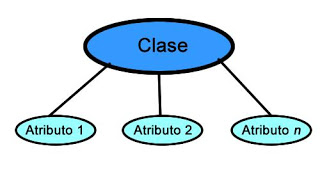
\includegraphics[scale=0.6]{nive}
\par\end{centering}
\caption{Representación gráfica del algoritmo Naive Bayes.}
\end{figure}
Se ejecutó el algoritmo Naive Bayes en Weka para crear los clasificadores de las distintas vistas minables. Los resultados se muestran en la tabla \ref{tab:cuadro36}

\begin{longtable}{|p{3cm}|p{3cm}|p{2cm}|p{2cm}|p{2cm}|p{2cm}|}
%\centering
%\begin{tabular}{|p{3cm}|p{3cm}|p{2cm}|p{2cm}|p{2cm}|p{2cm}|}
\hline
	\rowcolor[gray]{0.5} 
	\multicolumn{2}{|c|}{Vista minable} &
	\multicolumn{4}{|c|}{Porcentaje de éxito de las instancias clasificadas}\\
	\hline
	\rowcolor[gray]{0.9} 
	Nombre & \# de instancias & 100\% & 90\% & 80\% & 70\%\\
	\hline
	\endhead
	\hline
	\multicolumn{6}{r}{\textit{Continua en la siguiente pagina.}} \\
	\endfoot
	\endlastfoot
\multirow{3}[5]{*}{Biologia9} & 1000  & 444   & 479   & 70    & 6 \\
\cline{2-6}      & 10000 & 442   & 480   & 71    & 7 \\
\cline{2-6}      & 100000 & 450   & 478   & 68    & 4 \\
\hline
\multirow{3}[6]{*}{Biologia10} & 1000  & 340   & 475   & 148   & 34 \\
\cline{2-6}      & 10000 & 242   & 423   & 243   & 78 \\
\cline{2-6}      & 100000 & 183   & 325   & 222   & 100 \\
\hline
\multirow{3}[6]{*}{Filosofia7} & 1000  & 374   & 441   & 140   & 38 \\
\cline{2-6}      & 10000 & 287   & 467   & 181   & 47 \\
\cline{2-6}      & 100000 & 226   & 416   & 192   & 92 \\
\hline
\multirow{3}[6]{*}{Fisica11} & 1000  & 348   & 440   & 179   & 28 \\
\cline{2-6}      & 10000 & 259   & 365   & 234   & 108 \\
\cline{2-6}      & 100000 & 185   & 289   & 263   & 193 \\
\hline
\multirow{3}[6]{*}{Fisica112} & 1000  & 340   & 411   & 198   & 46 \\
\cline{2-6}      & 10000 & 229   & 349   & 247   & 131 \\
\cline{2-6}      & 100000 & 192   & 252   & 226   & 214 \\
\hline
\multirow{2}[4]{*}{Ingles11} & 1000  & 441   & 432   & 85    & 17 \\
\cline{2-6}      & 10000 & 452   & 418   & 84    & 14 \\
\hline
\multirow{3}[6]{*}{Lenguaje10} & 1000  & 309   & 454   & 198   & 37 \\
\cline{2-6}      & 10000 & 209   & 347   & 274   & 125 \\
\cline{2-6}      & 100000 & 125   & 224   & 239   & 194 \\
\hline
\multirow{3}[6]{*}{Lenguaje102} & 1000  & 555   & 397   & 46    & 2 \\
\cline{2-6}      & 10000 & 478   & 467   & 52    & 3 \\
\cline{2-6}      & 100000 & 437   & 487   & 68    & 6 \\
\hline
\multirow{3}[6]{*}{Matematica10} & 1000  & 244   & 429   & 187   & 91 \\
\cline{2-6}      & 10000 & 200   & 351   & 205   & 111 \\
\cline{2-6}      & 100000 & 190   & 296   & 197   & 142 \\
\hline
\multirow{3}[6]{*}{Matematica102} & 1000  & 279   & 449   & 197   & 61 \\
\cline{2-6}      & 10000 & 274   & 439   & 217   & 60 \\
\cline{2-6}      & 100000 & 246   & 454   & 214   & 78 \\
\hline
\multirow{3}[6]{*}{MedioAmbiente5} & 1000  & 255   & 582   & 154   & 2 \\
\cline{2-6}      & 10000 & 191   & 540   & 143   & 12 \\
\cline{2-6}      & 100000 & 169   & 486   & 144   & 95 \\
\hline
\multirow{3}[6]{*}{MedioAmbiente7} & 1000  & 205   & 561   & 137   & 13 \\
\cline{2-6}      & 10000 & 123   & 380   & 265   & 122 \\
\cline{2-6}      & 100000 & 78    & 279   & 199   & 219 \\
\hline
\multirow{3}[6]{*}{ProBiologia6} & 1000  & 212   & 398   & 313   & 62 \\
\cline{2-6}      & 10000 & 217   & 398   & 309   & 61 \\
\cline{2-6}      & 50000 & 210   & 401   & 307   & 71 \\
\hline
\multirow{3}[6]{*}{ProBiologia8} & 1000  & 234   & 372   & 299   & 80 \\
\cline{2-6}      & 10000 & 219   & 366   & 286   & 107 \\
\cline{2-6}      & 50000 & 222   & 375   & 279   & 99 \\
\hline
\multirow{3}[6]{*}{ProLenguaje7} & 1000  & 194   & 554   & 227   & 22 \\
\cline{2-6}      & 10000 & 204   & 546   & 235   & 14 \\
\cline{2-6}      & 50000 & 192   & 540   & 246   & 19 \\
\hline
\multirow{3}[6]{*}{ProLenguaje9} & 1000  & 196   & 533   & 242   & 24 \\
\cline{2-6}      & 10000 & 214   & 518   & 244   & 17 \\
\cline{2-6}      & 50000 & 196   & 511   & 251   & 35 \\
\hline
\multirow{3}[6]{*}{ProMatematica7} & 1000  & 262   & 582   & 122   & 25 \\
\cline{2-6}      & 10000 & 290   & 556   & 110   & 32 \\
\cline{2-6}      & 50000 & 339   & 494   & 128   & 30 \\
\hline
\multirow{3}[6]{*}{ProMatematica9} & 1000  & 262   & 536   & 147   & 44 \\
\cline{2-6}      & 10000 & 311   & 501   & 129   & 48 \\
\cline{2-6}      & 50000 & 295   & 504   & 136   & 52 \\
\hline
\multirow{3}[6]{*}{ProSociales7} & 1000  & 166   & 611   & 208   & 12 \\
\cline{2-6}      & 10000 & 214   & 564   & 206   & 14 \\
\cline{2-6}      & 50000 & 210   & 565   & 208   & 13 \\
\hline
\multirow{3}[6]{*}{ProSociales9} & 1000  & 254   & 532   & 192   & 17 \\
\cline{2-6}      & 10000 & 209   & 551   & 224   & 13 \\
\cline{2-6}      & 50000 & 199   & 543   & 227   & 27 \\
\hline
\multirow{3}[6]{*}{Quimica10} & 1000  & 397   & 382   & 187   & 32 \\
\cline{2-6}      & 10000 & 285   & 370   & 238   & 79 \\
\cline{2-6}      & 100000 & 225   & 258   & 232   & 172 \\
\hline
\multirow{3}[6]{*}{Sociales7} & 1000  & 401   & 493   & 94    & 11 \\
\cline{2-6}      & 10000 & 369   & 445   & 150   & 33 \\
\cline{2-6}      & 100000 & 349   & 426   & 162   & 41 \\
\hline
\multirow{3}[6]{*}{Sociales9} & 1000  & 332   & 484   & 146   & 34 \\
\cline{2-6}      & 10000 & 263   & 424   & 254   & 50 \\
\cline{2-6}      & 100000 & 186   & 358   & 245   & 104 \\
\hline
\multirow{3}[6]{*}{Violencia11} & 1000  & 295   & 368   & 179   & 82 \\
\cline{2-6}      & 10000 & 214   & 316   & 187   & 137 \\
\cline{2-6}      & 100000 & 160   & 241   & 163   & 181 \\
\hline
\caption{Resultados de la construcción y evaluación de las vistas minables usando el algoritmo Naive Bayes.}
\label{tab:cuadro36}
\end{longtable}
Este algoritmo a diferencia de los anteriores mostró una menor confianza, por encima del 80\% de precisión estaban, en general, alrededor de 70\% de las instancias evaluadas, pero algunos clasificadores si tuvieron un nivel de confianza mayor.

En general el algoritmo presenta muchas variaciones en sus clasificaciones y por tanto su confianza no es tan acertada como lo fue, por ejemplo, la del algoritmo de los k vecinos más cercanos.
\subsection{Funciones de base radial}
El algoritmo de creación de clasificadores utilizando la red de Funciones de Base Radial o RBF (Radial Basis Function) se encuentra implementado en Weka en la librería RBFNetwork\footnote{\url{ http://weka.sourceforge.net/doc.stable/weka/classifiers/functions/RBFNetwork.html}}.

Las redes neuronales artificiales (RNA) tienen distintas aplicaciones, entre ellas se encuentra la clasificación \cite{key-250}. Su objetivo es tratar de emular la capacidad humana de procesar información.  

Las RNA pueden ser entrenadas usando métodos de aprendizaje supervisado o no supervisado \cite{key-240}. Una de las redes encontradas en el aprendizaje supervisado es la red de Funciones de Base Radial. Las redes RBF constan de 3 capas, en la primera se reciben los atributos de entrada a ser clasificados, en la segunda capa o capa oculta se utiliza una función de calculo para realizar la transformación, no lineal, desde el espacio de la capa de entrada al espacio de la capa intermedia. En la tercera capa se encuentra los valores posibles de la clase a clasificar. 

\begin{figure}[H]
\begin{centering}
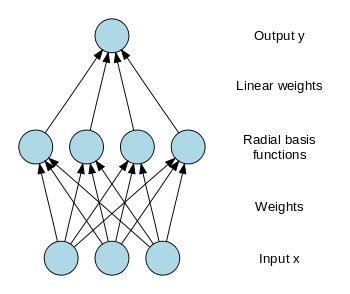
\includegraphics[scale=0.6]{rbf}
\par\end{centering}
\caption{Estructura de las capas de una red neuronal de funciones de base radial.}
\end{figure}
Se realizo la creación de los clasificadores utilizando las vistas minables. Los resultados se muestran en la tabla \ref{tab:cuadro37}

\begin{longtable}{|p{3cm}|p{3cm}|p{2cm}|p{2cm}|p{2cm}|p{2cm}|}
%\centering
%\begin{tabular}{|p{3cm}|p{3cm}|p{2cm}|p{2cm}|p{2cm}|p{2cm}|}
\hline
	\rowcolor[gray]{0.5} 
	\multicolumn{2}{|c|}{Vista minable} &
	\multicolumn{4}{|c|}{Porcentaje de éxito de las instancias clasificadas}\\
	\hline
	\rowcolor[gray]{0.9} 
	Nombre & \# de instancias & 100\% & 90\% & 80\% & 70\%\\
	\hline
	\endhead
	\hline
	\multicolumn{6}{r}{\textit{Continua en la siguiente pagina.}} \\
	\endfoot
	\endlastfoot
\multirow{3}[5]{*}{Biologia9} & 1000  & 434   & 485   & 73    & 7 \\
\cline{2-6}      & 10000 & 456   & 486   & 52    & 5 \\
\cline{2-6}      & 100000 & 466   & 477   & 52    & 2 \\
\hline
\multirow{3}[6]{*}{Biologia10} & 1000  & 347   & 439   & 120   & 63 \\
\cline{2-6}      & 10000 & 362   & 441   & 151   & 29 \\
\cline{2-6}      & 100000 & 422   & 427   & 96    & 14 \\
\hline
\multirow{3}[6]{*}{Filosofia7} & 1000  & 309   & 448   & 192   & 45 \\
\cline{2-6}      & 10000 & 376   & 476   & 97    & 30 \\
\cline{2-6}      & 100000 & 382   & 497   & 98    & 22 \\
\hline
\multirow{3}[6]{*}{Fisica11} & 1000  & 273   & 321   & 92    & 78 \\
\cline{2-6}      & 10000 & 408   & 445   & 110   & 34 \\
\cline{2-6}      & 100000 & 523   & 396   & 68    & 9 \\
\hline
\multirow{3}[6]{*}{Fisica112} & 1000  & 416   & 428   & 132   & 21 \\
\cline{2-6}      & 10000 & 473   & 426   & 82    & 16 \\
\cline{2-6}      & 100000 & 441   & 420   & 97    & 32 \\
\hline
\multirow{2}[4]{*}{Ingles11} & 1000  & 407   & 440   & 90    & 28 \\
\cline{2-6}      & 10000 & 440   & 439   & 68    & 18 \\
\hline
\multirow{3}[6]{*}{Lenguaje10} & 1000  & 258   & 385   & 289   & 60 \\
\cline{2-6}      & 10000 & 443   & 420   & 86    & 35 \\
\cline{2-6}      & 100000 & 459   & 366   & 97    & 58 \\
\hline
\multirow{3}[6]{*}{Lenguaje102} & 1000  & 507   & 409   & 70    & 11 \\
\cline{2-6}      & 10000 & 567   & 389   & 42    & 2 \\
\cline{2-6}      & 100000 & 563   & 408   & 27    & 2 \\
\hline
\multirow{3}[6]{*}{Matematica10} & 1000  & 216   & 380   & 195   & 85 \\
\cline{2-6}      & 10000 & 296   & 504   & 147   & 45 \\
\cline{2-6}      & 100000 & 340   & 520   & 109   & 18 \\
\hline
\multirow{3}[6]{*}{Matematica102} & 1000  & 317   & 449   & 171   & 43 \\
\cline{2-6}      & 10000 & 342   & 480   & 142   & 24 \\
\cline{2-6}      & 100000 & 355   & 494   & 117   & 24 \\
\hline
\multirow{3}[6]{*}{MedioAmbiente5} & 1000  & 183   & 677   & 121   & 0 \\
\cline{2-6}      & 10000 & 196   & 668   & 127   & 0 \\
\cline{2-6}      & 100000 & 166   & 679   & 83    & 32 \\
\hline
\multirow{3}[6]{*}{MedioAmbiente7} & 1000  & 242   & 643   & 81    & 1 \\
\cline{2-6}      & 10000 & 257   & 644   & 86    & 5 \\
\cline{2-6}      & 100000 & 135   & 640   & 137   & 20 \\
\hline
\multirow{3}[6]{*}{ProBiologia6} & 1000  & 200   & 390   & 301   & 94 \\
\cline{2-6}      & 10000 & 242   & 410   & 280   & 55 \\
\cline{2-6}      & 50000 & 262   & 419   & 274   & 36 \\
\hline
\multirow{3}[6]{*}{ProBiologia8} & 1000  & 233   & 366   & 277   & 96 \\
\cline{2-6}      & 10000 & 268   & 396   & 259   & 62 \\
\cline{2-6}      & 50000 & 281   & 397   & 253   & 59 \\
\hline
\multirow{3}[6]{*}{ProLenguaje7} & 1000  & 211   & 546   & 209   & 28 \\
\cline{2-6}      & 10000 & 199   & 559   & 229   & 12 \\
\cline{2-6}      & 50000 & 208   & 560   & 221   & 10 \\
\hline
\multirow{3}[6]{*}{ProLenguaje9} & 1000  & 226   & 531   & 227   & 9 \\
\cline{2-6}      & 10000 & 217   & 548   & 222   & 8 \\
\cline{2-6}      & 50000 & 220   & 543   & 222   & 9 \\
\hline
\multirow{3}[6]{*}{ProMatematica7} & 1000  & 279   & 561   & 111   & 31 \\
\cline{2-6}      & 10000 & 309   & 568   & 90    & 22 \\
\cline{2-6}      & 50000 & 268   & 622   & 78    & 23 \\
\hline
\multirow{3}[6]{*}{ProMatematica9} & 1000  & 315   & 499   & 130   & 36 \\
\cline{2-6}      & 10000 & 248   & 574   & 96    & 38 \\
\cline{2-6}      & 50000 & 251   & 606   & 98    & 35 \\
\hline
\multirow{3}[6]{*}{ProSociales7} & 1000  & 188   & 565   & 211   & 30 \\
\cline{2-6}      & 10000 & 191   & 584   & 208   & 12 \\
\cline{2-6}      & 50000 & 181   & 613   & 192   & 10 \\
\hline
\multirow{3}[6]{*}{ProSociales9} & 1000  & 244   & 524   & 206   & 19 \\
\cline{2-6}      & 10000 & 185   & 599   & 204   & 9 \\
\cline{2-6}      & 50000 & 177   & 608   & 203   & 7 \\
\hline
\multirow{3}[6]{*}{Quimica10} & 1000  & 431   & 411   & 126   & 28 \\
\cline{2-6}      & 10000 & 450   & 394   & 141   & 14 \\
\cline{2-6}      & 100000 & 459   & 424   & 77    & 26 \\
\hline
\multirow{3}[6]{*}{Sociales7} & 1000  & 370   & 486   & 125   & 17 \\
\cline{2-6}      & 10000 & 377   & 419   & 96    & 30 \\
\cline{2-6}      & 100000 & 469   & 434   & 87    & 7 \\
\hline
\multirow{3}[6]{*}{Sociales9} & 1000  & 369   & 505   & 114   & 8 \\
\cline{2-6}      & 10000 & 413   & 462   & 112   & 12 \\
\cline{2-6}      & 100000 & 398   & 480   & 93    & 19 \\
\hline
\multirow{3}[6]{*}{Violencia11} & 1000  & 268   & 380   & 200   & 86 \\
\cline{2-6}      & 10000 & 374   & 423   & 129   & 45 \\
\cline{2-6}      & 100000 & 323   & 380   & 161   & 91 \\
\hline
\caption{Resultados de la construcción y evaluación de las vistas minables usando el algoritmo RBF.}
\label{tab:cuadro37}
\end{longtable}
En los clasificadores construidos con redes RBF se puede notar de nuevo una mejora en la calidad de la predicciones. Al momento de clasificar las instancias de entrenamiento, en todos los clasificadores construidos se logra una predicción del 80\% de precisión en más del 90\% de las instancias de evaluación.

También en este clasificador se observó una tendencia más marcada en algunos clasificadores a mejorar la calidad de sus precisiones a medida que se incrementaba la cantidad de instancias de entrenamientos. 

En conclusión, los clasificadores con este algoritmo, también generaron una buena confianza con la calidad de sus resultados.
\section{Selección de los clasificadores}
Teniendo en cuenta los resultados que obtuvieron cada uno de los clasificadores con cada una de las vistas minables presentadas por las áreas académicas, se eligieron los mejores resultados por cada una.

La elección de los mejores clasificadores se realizó comparando primero cuál de los clasificadores clasificaba más instancias con un 100\% de precisión, si existían 2 o más con la misma cantidad de instancias en este valor, se elegía el que tuviera más instancias clasificadas con un 90\% de precisión y así sucesivamente.

Teniendo en cuenta este criterio y los resultados relacionados en las tablas anteriores, los clasificadores seleccionados se relacionan en la tabla \ref{tab:cuadro38}.

\begin{table}[!Hhtb]
\centering
\begin{tabular}{|p{6.5cm}|p{3cm}|p{3cm}|p{3cm}|}
\hline
	\rowcolor[gray]{0.9} 
	\textbf{Área académica} &
	\textbf{Vista minable} &
	\textbf{Instancias de entrenamiento} &
	\textbf{Algoritmo del clasificador}
	\\
\hline
Biología & Biologia9 & 100.000 & Redes RBF \\
\hline
Ciencias Sociales & Sociales7 & 100.000 & Redes RBF \\
\hline
Filosofia & Filosofia7 & 10.000 & KNN K=2 \\
\hline
Fisica & Fisica11 & 100.000 & Redes RBF \\
\hline
Ingles & Ingles11 & 10.000 & KNN K=2 \\
\hline
Lenguaje & Lenguaje102 & 10.000 & Redes RBF \\
\hline
Matematica & Matematica10 & 10.000 & KNN K=1 \\
\hline
Medio Ambiente & MedioAmbiente5 & 1.000 & Naive Bayes \\
\hline
Profundizacion en Biologia & ProBiologia8 & 100.000 & Redes RBF \\
\hline
Profundizacion en Lenguaje & ProLenguaje9 & 1.000 & KNN K=2 \\
\hline
Profundizacion en Matematica & ProMatematica7 & 1.000 & KNN K=2 \\
\hline
Profundizacion en Ciencias Sociales & ProSociales7 & 1.000 & KNN K=2 \\
\hline
Quimica & Quimica10 & 10.000 & KNN K=1 \\
\hline
Violencia y Sociedad & Violencia11 & 10.000 & Redes RBF \\
\hline
\end{tabular}
\caption{Clasificadores seleccionados para la construcción de la interfaz de consultas.}
\label{tab:cuadro38}
\end{table}
%\include{clasificadores2}
\chapter{Construcción de la Interfaz de Consultas}
Después de haber seleccionado cuales serían los clasificadores que se utilizarían para realizar las predicciones en cada una de las áreas académicas, se debió tomar la decisión de cuál sería la mejor manera de presentar una interfaz de consultas, para que un usuario pudiera consultar cual sería el posible puntaje que obtendría un evaluado en cada una de las áreas académicas.

El primer aspecto a tener en cuenta era la interpretación de los clasificadores construidos. Weka permite guardar, en un archivo codificado, la estructura de un clasificador entrenado, para posteriormente utilizarlos con instancias de pruebas. Pero estos archivos codificados solo pueden ser cargados por las librerías de Weka. Es decir, que para poder utilizar los clasificadores creados, en la aplicación se debían utilizar estas librerías, por lo tanto el lenguaje base de la aplicación debía ser Java\footnote{\url{http://www.java.com}}.

El segundo aspecto que se tuvo en cuenta para la construcción de la interfaz, fue que analizando las vistas minables seleccionadas y realizando una intersección entre los atributos de los que estaba compuesta cada una, se tenía un total de 18 parámetros a preguntar. Esta cantidad de parámetros podrían ser fácilmente indagados en un formulación en HTML, además de que, una aplicación de escritorio en donde se tenga solo un formulario para obtener una respuesta es poco llamativo y se podría obtener un mayor acceso de usuarios si esta interfaz está construida sobre un entorno web.

Las ventajas que se obtienen con aplicaciones web son por ejemplo: que pueden ser accedidas siempre, sin importar en que dispositivos el usuario se encuentre: computador, laptop, tableta o teléfono inteligente. Se ejecutan sin importar el sistema operativo del usuario, no requieren instalación, entre otras.

Así, conociendo los 2 aspectos más importantes que debía cumplir la aplicación, se decidió utilizar la plataforma de programación J2EE de Java, la cual permite la creación de Servlets, los cuales son archivos de código Java que se ejecutan dentro de un contenedor de Servlets \cite{key-260}.

Los contenedores de Servlets capturan las peticiones que un usuario realiza sobre un servicio web y se encarga de procesar esta solicitud, enviársela al Servlet que procesa los datos y retorna una respuesta que de nuevo es procesa por el contenedor y entregada al navegador para que el usuario pueda visualizar los resultados de su petición.

Para la interfaz de navegación del usuario se utilizó la tecnología AJAX (Asynchronous JavaScript And XML). AJAX oficialmente es definido como: \begin{quote}“AJAX no es una tecnología en sí mismo. En realidad, se trata de varias tecnologías independientes que se unen de formas nuevas y sorprendentes.” \cite{key-270}.\end{quote}

AJAX permite que las consultas que se realizan desde una interfaz HTML hacia un servidor se realicen de manera asíncrona, evitando así la recarga constante de la página, cada vez que se desea consultar algo. Esto habilita al usuario a realizar diferentes tareas al tiempo, sin perder la posibilidad de continuar interactuando con la página.
\section{Arquitectura}
La arquitectura usada para la construcción de la aplicación, fue una arquitectura Cliente-Servidor. Del lado del cliente se tiene la capa de presentación que se carga por medio de un navegador web, esta presentación está construida usando HTML y una hoja de estilo CSS3.

La conexión con el servidor de Servlets se realiza a través de JavaScritp usando la tecnología AJAX y la librería JQuery\footnote{\url{http://jquery.com/}} para manipular el comportamiento de los componentes gráficos de la presentación, como el intercambio de div’s y estado de inhabilidad de los botones.

En el servidor se encuentra el Servlet PrediXaber, que se encarga de recibir los datos ingresados por el usuario y construir con ellos los archivos arff a ser ejecutados en los clasificadores. Estos archivos arff son creados agregando los datos de entrada a una plantilla predefinida, que tiene la estructura de datos que concuerda con cada uno de los clasificadores construidos.

Utilizando el archivo arff creado, se procede a cargar cada uno de los clasificadores usando las librerías de Weka, se ejecuta la clasificación por cada una de las áreas académicas y se construye una respuesta que es enviada, de nuevo, a través de AJAX. Esta respuesta se recibe y es cargada en la página HTML para que el usuario pueda observar los resultados de la consulta.

La figura \ref{fig:figura3} muestra gráficamente el diseño de la arquitectura de la aplicación.

\begin{figure}[!htb]
\begin{centering}
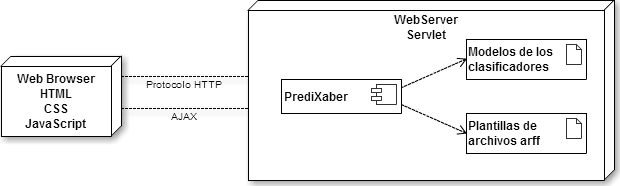
\includegraphics[scale=0.65]{package}
\par\end{centering}
\caption{Diseño arquitectónico de la aplicación.}
\label{fig:figura3}
\end{figure}
\section{Flujo de navegación}
El flujo de navegación normal que se debe seguir en la aplicación, es cargar la página principal donde se muestra el formulario con los campos requeridos para realizar la consulta. Después de  ingresar la información correspondiente al evaluado, se procede a enviar este formulario para que sea procesado en el servidor. La respuesta es retornada desde el servidor y desplegada en la pantalla para que el usuario pueda conocer los resultados de su consulta.

\begin{figure}[!htb]
\begin{centering}
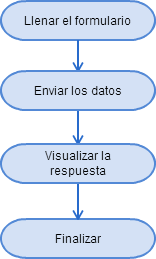
\includegraphics[scale=0.65]{Flowchart}
\par\end{centering}
\caption{Flujo normal de navegación que se sigue en la aplicación.}
\label{fig:figura4}
\end{figure}
\section{Codificación}
El proceso de codificación de la aplicación, se realizó utilizando los lenguajes programación Java y JavaScript, en Java se hizo uso de la librería Weka y en JavaScript de JQuery. Se utilizó HTML para definir los componentes de la página principal presentada al usuario y CSS3 para darle estilo a esos componentes.

En el ambiente de desarrollo se utilizó como IDE de desarrollo Eclipse\footnote{\url{http://www.eclipse.org}} y el contenedor de Servlets Tomcat\footnote{\url{http://tomcat.apache.org/}}.

Los parámetros que se envían al Servlet son procesados a través de un método POST para que la información sea enviada de manera codificada y no sea visible en la URL de la consulta. En el Servlet construido heredando la clase predefinida en java HttpServlet\footnote{\url{http://tomcat.apache.org/tomcat-7.0-doc/servletapi/javax/servlet/http/HttpServlet.html}} se construyó el método doPost() para procesar los datos recibidos y entregar una respuesta.

Dentro del Servlet la librería Weka se utilizó para la carga y ejecución de los clasificadores. Para cargar los archivos que contenían la información de los clasificadores se usó la clase SerializedClassifier, después de cargar la estructura, esta debía ser instanciada en un objeto del tipo Classifier para poder ejecutar el archivo arff. Se crea un objeto del tipo Instances que recibe como parámetro de construcción el BufferedReader que contiene el texto del archivo arff. Y por último, este objeto Instances es evaluado en el clasificador utilizando el método classifyInstance(), así se obtiene un valor para la clase a clasificar y este valor es retornado por medio del método doPost().

El código de la aplicación es sencillo, ya que solo se encarga de ejecutar las consultas usando los clasificadores anteriormente creados.
\section{Pruebas de usabilidad}
La usabilidad, en el software, se entiende como la facilidad que tiene un usuario de interactuar con la interfaz de las aplicaciones.

Los aspectos más importantes a evaluar en un diseño web son: curva de aprendizaje para el uso de la interfaz, eficacia de la interfaz, facilidad para memorizar, los errores que puede cometer el usuario y la satisfacción del usuario.

Para evaluar estos aspectos se hizo uso de la herramienta para evaluar usabilidad UsabilityHub\footnote{\url{https://usabilityhub.com/}}. Esta herramienta permita la creación de test que los usuarios pueden generar y compartir públicamente con las personas que ingresan a la página a responder estos test. 

Se hizo uso de 2 tipos de test. El test de Five Second, el cual le presenta al evaluador una imagen durante 5 segundos, después de ese tiempo realiza una pregunta que el evaluador debe responder. Y el test Click, el cual presenta una imagen acompañada de una pregunta en donde se le indica al evaluador que presione click en el lugar donde el cree que se ejecutaría cierta acción.

En el test de Five Second se presentó una imagen con el inicio de la página y se le pregunto al usuario sobre cual creía que era el objetivo de la página, después de leer la presentación. El 85\% de los encuestados, respondió que su finalidad era predecir resultados en la prueba saber 11\degree, el 15\% restantes, respondieron no tener clara la finalidad de la página.

En los test de Click se presentaron 3 imágenes, cada una con una pregunta sobre una acción a ejecutar. Las imágenes \ref{fig:figura5}, \ref{fig:figura6} y \ref{fig:figura7} muestra las preguntas realizadas y los resultados obtenidos.
\begin{figure}[!htb]
\begin{centering}
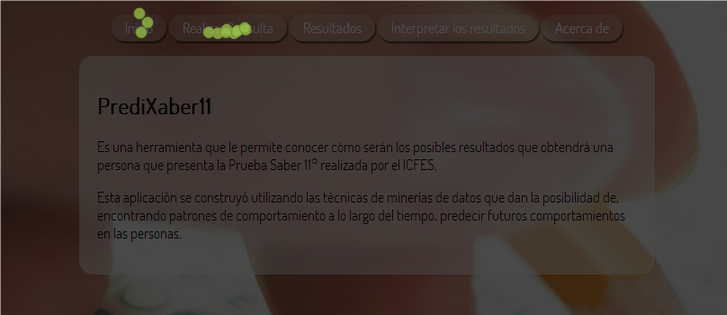
\includegraphics[scale=0.7]{realizarconsultatest2}
\par\end{centering}
\caption{Acción: Mira las opciones en los links y selecciona aquella que creas que te permitirá ejecutar una consulta.}
\label{fig:figura5}
\end{figure}
\begin{figure}[!htb]
\begin{centering}
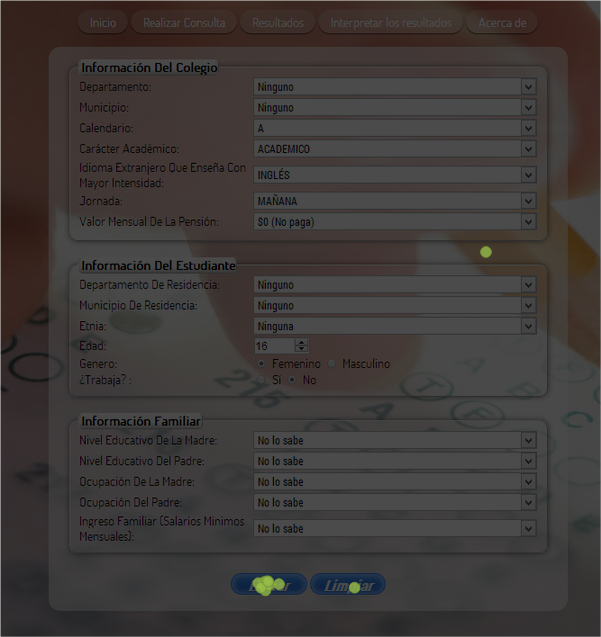
\includegraphics[scale=0.6]{enviarformulariotest}
\par\end{centering}
\caption{Acción: Donde harías click para enviar el formulario y recibir una respuesta.}
\label{fig:figura6}
\end{figure}
\begin{figure}[!htb]
\begin{centering}
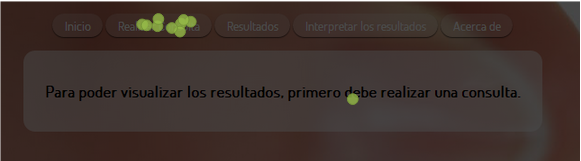
\includegraphics[scale=0.6]{realizarconsultatest}
\par\end{centering}
\caption{Acción: Donde harías click después de leer el mensaje.}
\label{fig:figura7}
\end{figure}
\section{Pruebas de código}
Para verificar la funcionalidad del código se generaron pruebas unitarias utilizando 2 frameworks diferentes pero conectables. Uno para evaluar que el flujo de navegación dentro de la aplicación retorne los resultados esperados y otro para evaluar que los métodos construidos dentro del Servlet funcionen correctamente al procesar la información recibida.
Para construir las pruebas del flujo de navegación se utilizó el framework de automatización de pruebas Selenium\footnote{\url{http://docs.seleniumhq.org/}}. Selenium permite grabar y reproducir pruebas a partir de un plugin que puede ser instalado en el navegador Firefox\footnote{\url{http://www.mozilla.org/en-US/firefox/new/}}. Con este plugin, el usuario inicia una grabación de pasos a seguir dentro del aplicativo web, entre cada paso ejecutado, el usuario puede agregar verificaciones de la respuesta o las respuesta esperadas al ejecutar ese paso.
Selenium también permite la ejecución de estas grabaciones, así cada vez que se desee verificar si los resultados esperados de una secuencia de pasos están siendo correctamente procesados, se ejecuta el script creado con anterioridad y se verifica este comportamiento.
Los scripts creados por Selenium pueden ser exportados a diferentes lenguajes de programación para ser ejecutados por otros frameworks de pruebas. Para el caso del presente trabajo, se decidió exportar el script creado al lenguaje de programación Java utilizando el framework de pruebas JUnit\footnote{\url{http://junit.org/}}.
Con JUnit también se construyeron tests para evaluar el comportamiento de los métodos definidos en el Servlet utilizado en el servidor para procesar las consultas del usuario. Se crearon 16 métodos de test en total que permiten verificar tanto el comportamiento de la interfaz de usuario y del código generado dentro de las clases.
\section{Pruebas de confiabilidad}
En esta prueba se quería comprobar la calidad de las predicciones realizadas por los clasificadores. Pero no individualmente, como ya se realizó, sino en conjunto ejecutando la solicitud al Servlet que realiza el procesamiento de los datos.

Para ejecutar esta prueba se utilizaron 100.000 registros de las bases de datos del año 2012, la cual ya se advirtió que no fue utilizada en la construcción de los clasificadores. Se creó un script en Python con el cual se ejecutaron las solicitudes al Servlet. A cada registro se le aplico la transformación de datos correspondiente.

Al recibir la respuesta de la solicitud se comparaban los resultados de las áreas académicas para encontrar en cuantas se realizaba correctamente la predicción.

La tabla \ref{tab:cuadro39} muestra los resultados de cuantas áreas académicas coincidieron. El total de áreas académicas en las que es evaluada una persona son 9, 8 de núcleo común y 1 de elección del evaluado.

\begin{table}[!Hhtb]
\centering
\begin{tabular}{|p{6.5cm}|p{6.5cm}|}
\hline
	\rowcolor[gray]{0.9} 
	\textbf{Cantidad de coincidencias} &
	\textbf{Cantidad de registros} 
	\\
\hline
9 & 98\\
\hline
8 & 881\\
\hline
7 & 3840\\
\hline
6 & 10116\\
\hline
5 & 17952\\
\hline
4 & 22166\\
\hline
3 & 20713\\
\hline
2 & 14598\\
\hline
1 & 8602\\
\hline
0 & 1034\\
\hline
\end{tabular}
\caption{Resultados de la prueba de confiabilidad realizada a la aplicación.}
\label{tab:cuadro39}
\end{table}
Se puede observar que cerca del 33\% de los registros evaluados (32.887) tienen al menos 5 coincidencias, que son más de la mitad de los puntajes a predecir. Se percibe que al momento de realizar consultas en conjunto sobre los clasificadores se pierde la calidad que estos mostraban de manera individual. Pero también se puede observar que las predicciones se comportan como una función gaussiana en  donde la mayoría de los resultados están agrupados en predicciones con el 50\% de confianza.
\chapter{Conclusiones y Trabajos Futuros}
\section{Conclusiones}
\begin{itemize}
\item Se logró aplicar el proceso de minería de datos a la información suministrada por el ICFES, logrando construir clasificadores que permitieron la elaboración de una interfaz de consultas donde los usuarios podrán conocer previamente sus resultados.

\item La suite de algoritmos de minería de datos Weka, es de gran utilidad en los procesos de descubrimiento del conocimiento en bases de datos. Su gran variedad de métodos que permiten realizar desde la selección de atributos, hasta algoritmos de clasificación construidos con distintas técnicas, hacen de esta herramienta un apoyo fundamental y que debería ser usada cuando se desarrollen proyectos de este tipo.
 
\item En el caso de estudio, la creación de los clasificadores, requirió de gran ayuda de parte del desarrollador, para la selección de los más apropiados acorde a los atributos predictores. Se notó que al aplicar cambios sencillos en la selección de los atributos predictores, los clasificadores mostraban cambios drásticos en sus predicciones. Los algoritmos de construcción de clasificadores son sensibles al cambio de su estructura de entrenamiento. Con agregar o retirar un atributo en el conjunto de entrenamiento, la calidad de las predicciones variaba significativamente.

\item El marco metodológico seguido en durante el proyecto \cite{key-50}, da una guía clara y útil a la hora de desarrollar proyectos de minería de datos, sus pasos son perfectamente explicados y se ajustaron precisamente a cada uno de los objetivos planteados  y contribuyeron al cumplimiento de cada uno de estos.

\item No se pudo encontrar un clasificador mejor o peor que otro, a excepción del algoritmo C4.5 el cual no genero resultados confiables. Todos los clasificadores tuvieron rendimientos confiables, pero algunos obtuvieron mejor rendimiento en ciertas áreas académicas. Esto se debe a que los algoritmos de clasificación tienen propiedades, en las que dependiendo el formato de los atributos predictores, generan una mayor calidad al momento de realizar las predicciones.

\item El proceso de desarrollo del proyecto agrupó el mayor esfuerzo en la construcción de los clasificadores. La construcción de la interfaz de consulta fue sencilla, además de que se optó por un entorno web, en el que la codificación de las interfaces es simple y no requiere del uso de máquinas con requerimientos específicos.

\item A pesar de que al evaluar la confiabilidad de la aplicación, la cantidad de clasificaciones que cumplieron con predecir correctamente todas las áreas académicas fue realmente baja, se obtuvieron resultados positivos al menos para el 50\% de las áreas académicas, además de que individualmente la calidad de las predicciones de los clasificadores estuvo por encima del 70\% de precisión.

\item La interfaz de consultas que se construyó, constó del uso de las tecnologías actuales en el desarrollo web. Como lo son componentes gráficos de HTML5 y CSS3, además de la aplicación de AJAX que permite al usuario interactuar de una manera más confortable con la interfaz de consultas.

\item El tiempo que tarda un clasificador en procesar una consulta y retornar una respuesta no presentó grandes diferencias entre los distintos algoritmos utilizados. Principalmente en la construcción de los clasificadores, el algoritmo C4.5 fue el que más tiempo demoró en generar el clasificador. Pero en el momento de resolver consultas, todos los algoritmos tomaron tiempos muy similares.

\item Los criterios de Precisión y Exhaustividad, que fueron tomados para evaluar la calidad de los resultados, presentaron en la mayoría de los clasificadores un comportamiento muy similar entre su valor. Pero principalmente se destacó que los algoritmos presentaban un poco de mayor exhaustividad que precisión. Esto no afectó la decisión de elegir los algoritmos que obtuvieran una mayor precisión en cada una de las pruebas aplicadas.

Se destaca también que la precisión alcanzo niveles mayores en los clasificadores que predecían áreas académicas de las pruebas del componente flexible. Esto se puede dar a que en el caso de estas pruebas, cada estudiante tiene la opción de elegir el área en la que se sienta mejor capacitado, generando esto en que esta área los puntajes sean de un promedio más alto.
\end{itemize}
\section{Trabajos futuros}
\begin{itemize}
\item El ICFES además de poner a disposición las bases de datos de los resultados en la prueba Saber 11\degree, también permite el acceso a los resultados en las pruebas Saber 3\degree, Saber 5\degree, Saber 9\degree y SaberPro. Siguiendo una propuesta metodológica similar a la aplicada en este trabajo, se pueden construir clasificadores que permitan predecir puntajes en estas pruebas.

\item Además de clasificadores, la minería de datos también permite la creación de otro tipo de utilidades que ayudan a encontrar patrones de comportamiento, por ejemplo los algoritmos de agrupamiento y los de asociación. Con las bases de datos homogeneizadas en este trabajo, se puede proceder a aplicar estos algoritmos para hallar reglas de comportamiento en los datos.

\item Las instituciones académicas pueden tener la iniciativa de desarrollar proyectos similares a este, en donde los datos sean más específicos a las particularidades de sus estudiantes. Así, con una mayor precisión en la información recolectada, las predicciones tendrán una mejor  calidad y se podrán aplicar con más efectividad refuerzos a los estudiantes para mejorar sus puntajes en la prueba.
\end{itemize}
\begin{thebibliography}{Referencias}
\bibitem{key-1}\foreignlanguage{english}{Periódico
El Colombiano, \textquotedblleft{}Leve mejoría en pruebas Saber 11\textquotedblright{}.
{[}artículo en Internet{]}}. \url{http://www.elcolombiano.com/BancoConocimiento/L/leve_mejoria_en_pruebas_saber_11/leve_mejoria_en_pruebas_saber_11.asp}\foreignlanguage{english}{
{[}Consulta: 24 agosto de 2012{]}.}

\bibitem{key-2}Periódico El Tiempo, \textquotedblleft{}El 45\% de
los colegios presentó bajo rendimiento en pruebas Saber 11\textquotedblright{}.
{[}artículo en Internet{]}\foreignlanguage{spanish}{. }\url{http://www.eltiempo.com/vida-de-hoy/educacion/ARTICULO-WEB-NEW\_NOTA\_INTERIOR-8384822.html}\foreignlanguage{spanish}{
}{[}Consulta: 24 agosto de 2012{]}.

\bibitem{key-3}Revista Dinero, \textquotedblleft{}Las pruebas del
Icfes no son el único indicador\textquotedblright{}. {[}artículo en
Internet{]}   \url{http://m.dinero.com/edicion-impresa/caratula/articulo/las-pruebas-del-icfes-no-unico-indicador/139069}
{[}Consulta: 14 marzo de 2012{]}.

\bibitem{key-4}Departamento Del Valle Del Cauca, Secretaria De Educación.
Informe Ejecutivo Análisis Pruebas Saber 5º, 9º Y 11º. Santiago de
Cali, Febrero 15 de 2012.

\bibitem{key-50}\foreignlanguage{spanish}{Hernández Orallo José,
Ramírez Quintana Ma. José, Ferri, Ramírez César, Introducción a la
minería de datos, Person Educación, S.A. Madrid 2004, ISBN: 978-84-205-4091-7.}

\selectlanguage{spanish}%
\bibitem{key-60}José C. Riquelme, Roberto Ruiz, Karina Gilbert, \textquotedblleft{}Minería
de Datos: Conceptos y Tendencias,\textquotedblright{} \emph{Revista
Iberoamericana de Inteligencia Artificial}, No. 29 (2006), pp. 11-18.

\bibitem{key-80}ICFES, Presentación. {[}artículo en Internet{]} \url{http://www2.icfes.gov.co/informacion-institucional/informacion-general}
{[}Consulta: 4 junio de 2012{]}.

\bibitem{key-90}C.S.R. Prabhu, Data Warehousing Concepts, Techniques
Products and Applications, Prentice-Hall, India 2006, ISBN: 81-203-2068-9.

\bibitem{key-100}Timarán Pereira, Ricardo. Una lectura sobre deserción
universitaria en estudiantes de pregrado desde la perspectiva de la
minería de datos.Revista Científica Guillermo de Ockham, vol. 8, núm.
1, enero-junio, 2010, pp. 121-130.

\bibitem{key-110}Álvaro Jiménez Galindo, Hugo Álvarez García. Minería
de Datos en la Educación. Universidad Carlos III de Madrid.

\bibitem{key-120}Dr Ray Hoare, Using CHAID for classication problems,
en New Zealand Statistical Association 2004 conference, Wellington.

\bibitem{key-130}Sergio Valero Orea, Alejandro Salvador Vargas, Marcela
García Alonso. Minería de datos: predicción de la deserción escolar
mediante el algoritmo de árboles de decisión y el algoritmo de los
k vecinos más cercanos. Universidad Tecnológica de Izúcar de Matamoros,
Izúcar de Matamoros, Puebla, México. Recursos digitales para la educación
y la cultura volumen Kaambal. ISBN Volumen: 978-607-95446-1-4.

\bibitem{key-140}Erika Rodallegas Ramos, Areli Torres González, Beatriz
B. Gaona Couto, Erick Gastelloú Hernández, Rafael A. Lez ama Morales,
Sergio Valero Orea. Modelo predictivo para la determinación de causas
de reprobación mediante Minería de Datos. Universidad Tecnológica
de Izúcar de Matamoros, Mexico. Recursos digitales para la educación
y la cultura volumen Kaambal. ISBN Volumen: 978-607-95446-1-4.

\bibitem{key-150}Elena Gervilla García, Rafael Jiménez López, Juan
José Montaño Moreno, Albert Sesé Abad, Berta Cajal Blasco, Alfonso
Palmer Pol. La metodología del Data Mining. Una aplicación al consumo
de alcohol en adolescentes. Área de Metodología de las Ciencias del
Comportamiento. Departamento de Psicología. Universitat de les Illes
Balears. Adicciones, 2009, Vol. 21 Núm. 1, Págs. 65-80.

\bibitem{key-160}T.Jyothirmayi et. al., An Algorithm for Better Decision
Tree, International Journal on Computer Science and Engineering Vol.
02, No. 09, 2010, 2827-2830.

\bibitem{key-70}Téllez A., Extracción de Información con Algoritmos
de Clasificación {[}Tesis de Maestría{]}. Tonantzintla, Puebla, México.
Instituto Nacional de Astrofísica, Óptica y Electrónica. 2005.

\bibitem{key-280}Christopher D., Prabhakar Raghavan, Hinrich Schütze, Introduction to Information Retrieval, Cambridge University Press, 2008, ISBN: 978-0-521-86571-5.

\bibitem{key-170}\foreignlanguage{spanish}{Ross Quinlan, C4.5: Programs for Machine Learning, Morgan Kaufmann Publishers. San Mateo, CA 1993, ISBN: 1-55860-238-0.}

\bibitem{key-210}\foreignlanguage{spanish}{Ian H. Witten, Eibe Frank, Mark A. Hall, Data Mining
Practical Machine Learning
Tools and Techniques - 3rd ed., Morgan Kaufmann Publishers, 2011, ISBN: 978-0-12-374856-0.}

\bibitem{key-290}\foreignlanguage{spanish}{Tom Dietterich, Michael Kearns, Yishay Mansour, Applying the Weak Learning Framework to Understand and Improve C4.5 en In Proceedings of the Thirteenth International Conference on Machine Learning, Morgan Kaufmann Publishers, 1996, ISBN: 155860-419-7.}

\bibitem{key-220}Jon Louis Bentley, Multidimensional Binary Search Trees Used for Associative Searching, Communications of the ACM Vol. 18, No. 09, 1975, 509-517.

\bibitem{key-300}Wu et al, Top 10 Algorithms in Data Mining, Knowledge and Information Systems Vol. 14, No. 01, 2007, 1-37.

\bibitem{key-180}D. Aha, D. Kibler, Instance-based learning algorithms, Machine Learning Vol.
06, 1991, 37-66.

\bibitem{key-230}\foreignlanguage{spanish}{Mitchell T.M., Machine Learning, McGraw-Hill, 1997, ISBN: 0070428077.}

\bibitem{key-190}George H. John, Pat Langley, Estimating Continuous Distributions in Bayesian Classifiers, Eleventh Conference on Uncertainty in Artificial Intelligence, Morgan Kaufmann Publishers. San Mateo, CA 1995, 338-345, ISBN: 1-55860-385-9.

\bibitem{key-250}Guoqiang Peter Zhang, Neural Networks for Classification: A Survey, IEEE Transactions on systems, man, and cybernetics, Part c: Applications and reviews, vol. 30, no. 4, november 2000, 451-462.

\bibitem{key-240}\foreignlanguage{spanish}{Mohamad H. Hassoun, Fundamentals of Artificial Neural Networks, Massachusetts Institute of Technology, 1995, ISBN: 0262514672}

\bibitem{key-200}J. Park, I. W. Sandberg, Universal Approximation Using Radial-Basis-Function
Networks, Neural Computation Vol.
03, 1991, 246-257.

\bibitem{key-260}Benjamin Aumaille, J2EE Desarrollo de aplicaciones Web, Ediciones ENI, 2002, ISBN: 2-7460-1912-4.\bibitem{key-270}Nicholas C. Zakas, Jeremy McPeak, Joe Fawcett, Professional Ajax, 2nd Edition, Wiley Publishing, 2007, ISBN: 978-0-470-10949-6.\end{thebibliography}
%\documentclass{article}
\usepackage[utf8]{inputenc} 
\usepackage[spanish]{babel}
\usepackage{url} 
\usepackage{enumerate}
\usepackage{graphicx}
\usepackage{float}
\usepackage{multicol}
\usepackage[absolute,overlay]{textpos}
  \setlength{\TPHorizModule}{1mm}
  \setlength{\TPVertModule}{1mm}
\usepackage{colortbl}
\usepackage[colorlinks=true,linkcolor=black,urlcolor=black, citecolor=black]{hyperref}
\usepackage[top=30mm,bottom=30mm,inner=30mm,outer=20mm,asymmetric]{geometry}
\newcommand{\degree}{\ensuremath{^\circ}}
\begin{document}
\section*{Gráficas de resultados de la ejecución de los algoritmos con las vistas minables construidas.}
En este documento se presentan los resultados de ejecutar las vistas minables creadas en la sección 4.2 del trabajo de grado Aplicación para la predicción de resultados en la prueba Saber 11\degree.\\

Se presentan los valores de precisión y exhaustividad (Recall) que se obtuvo al ejecutar cada algoritmo con una cantidad de 1000  instancias contenidas en los archivos de evaluación. En el área derecha de cada gráfica se indica el significado de cada punto en la gráfica. Cada punto representa un algoritmo y la cantidad de instancias con las que se entrenó ese algoritmo. Por ejemplo, en la figura \ref{fig:figura1} se observa J48 – 1000, lo cual quiere decir que indica la precisión y la exhaustividad que obtuvo el algoritmo J48 entrenado con 1000 instancias.\\

Para el caso de los k vecinos más cercanos (IBK), se presentan los resultados tanto para la ejecución con k=1 como para la ejecución con k=2.\\

Los nombres de los algoritmos presentados en las gráficas, son los nombres de las librerías que los ejecutan en Weka. C4.5 es J48, k vecinos más cercanos es IBK, Naive Bayes es Naive y la red neural de funciones de base radial es RBF.\\
\begin{textblock}{80}(25,120)
\begin{figure}[!htb]
\begin{centering}
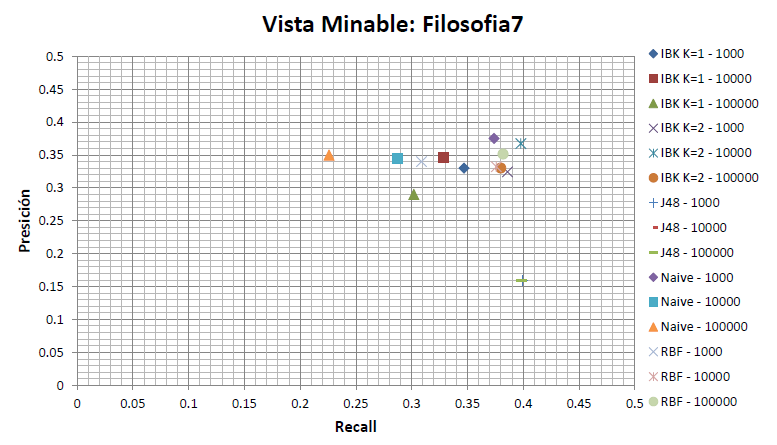
\includegraphics[scale=0.4]{filosofia7}
\par\end{centering}
\caption{Precision y recall obtenidos al evaluar los clasificadores entrenados usando la vista minable Filosofia7.}
\label{fig:figura1}
\end{figure}
\end{textblock}

\begin{textblock}{80}(110,120)
\begin{figure}[!htb]
\begin{centering}
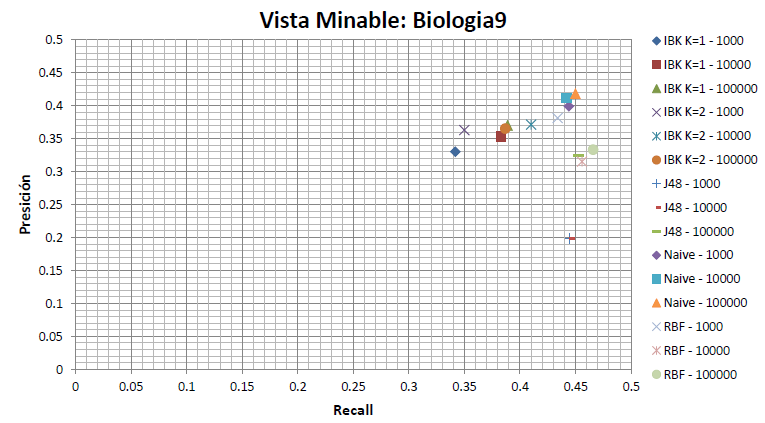
\includegraphics[scale=0.4]{biologia9}
\par\end{centering}
\caption{Precision y recall obtenidos al evaluar los clasificadores entrenados usando la vista minable Biologia9.}
\label{fig:figura2}
\end{figure}
\end{textblock}

\begin{textblock}{80}(25,186)
\begin{figure}[!htb]
\begin{centering}
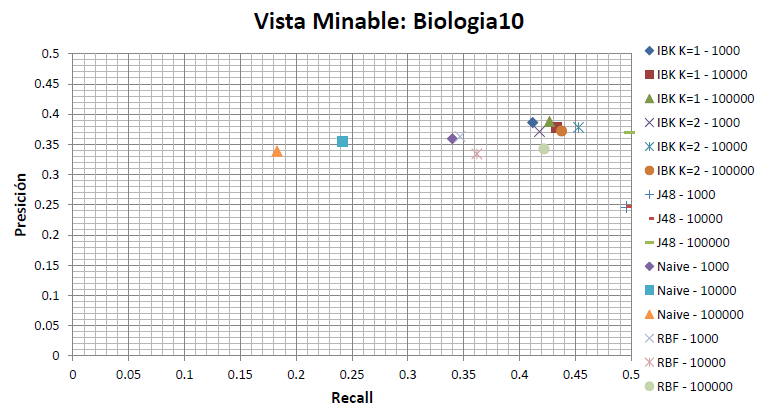
\includegraphics[scale=0.4]{biologia10}
\par\end{centering}
\caption{Precision y recall obtenidos al evaluar los clasificadores entrenados usando la vista minable Biologia10.}
\label{fig:figura3}
\end{figure}
\end{textblock}

\begin{textblock}{80}(110,185)
\begin{figure}[!htb]
\begin{centering}
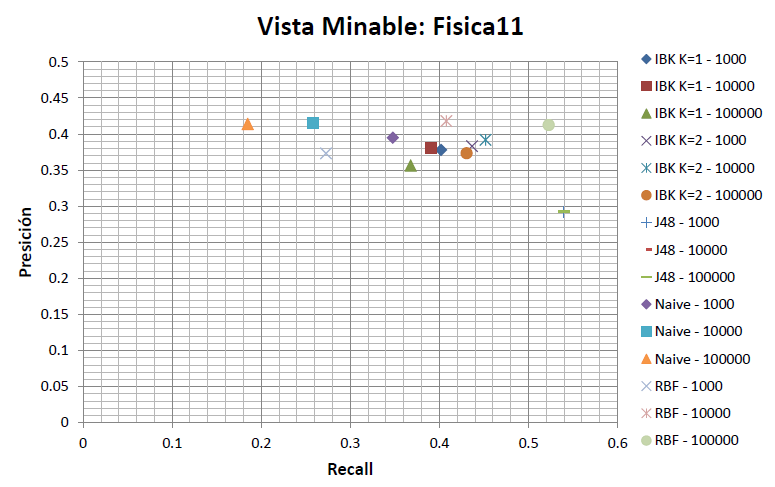
\includegraphics[scale=0.4]{fisica11}
\par\end{centering}
\caption{Precision y recall obtenidos al evaluar los clasificadores entrenados usando la vista minable Fisica11.}
\label{fig:figura4}
\end{figure}
\end{textblock}

\clearpage

\begin{textblock}{80}(25,30)
\begin{figure}[!htb]
\begin{centering}
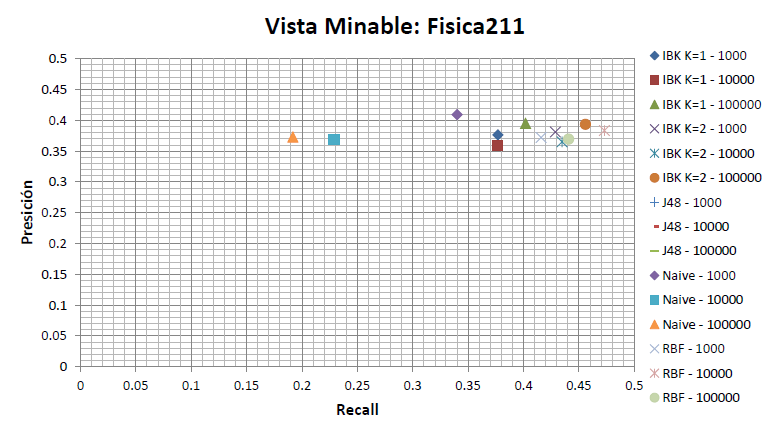
\includegraphics[scale=0.4]{fisica211}
\par\end{centering}
\caption{Precision y recall obtenidos al evaluar los clasificadores entrenados usando la vista minable Fisica211.}
\label{fig:figura5}
\end{figure}
\end{textblock}

\begin{textblock}{80}(110,30)
\begin{figure}[!htb]
\begin{centering}
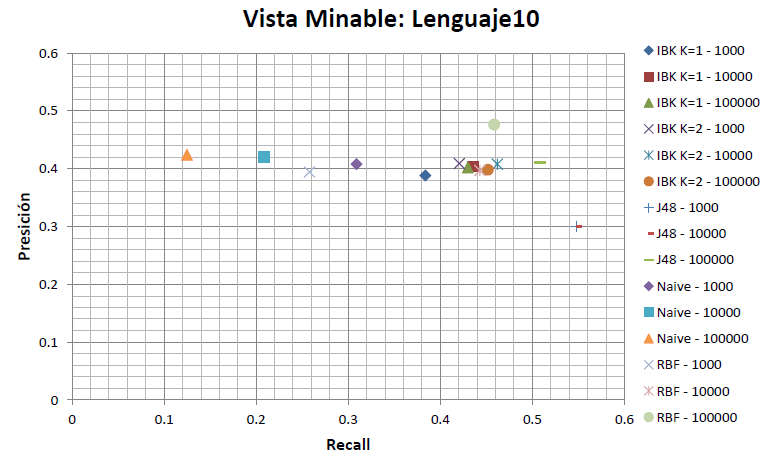
\includegraphics[scale=0.4]{lenguaje10}
\par\end{centering}
\caption{Precision y recall obtenidos al evaluar los clasificadores entrenados usando la vista minable Lenguaje10.}
\label{fig:figura6}
\end{figure}
\end{textblock}

\begin{textblock}{80}(25,100)
\begin{figure}[!htb]
\begin{centering}
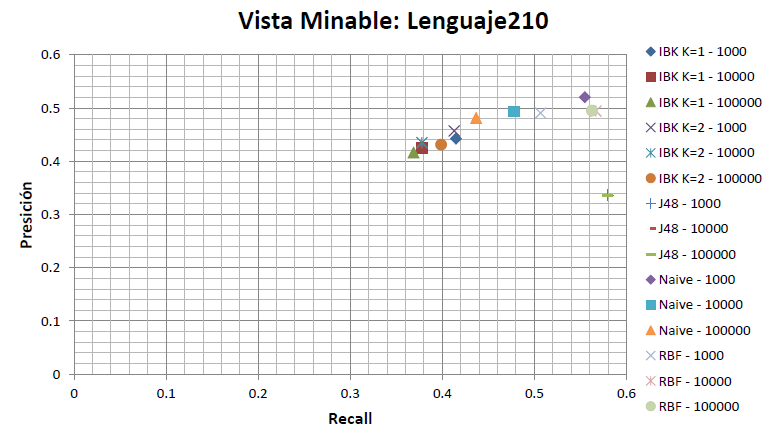
\includegraphics[scale=0.4]{lenguaje210}
\par\end{centering}
\caption{Precision y recall obtenidos al evaluar los clasificadores entrenados usando la vista minable Lenguaje210.}
\label{fig:figura7}
\end{figure}
\end{textblock}

\begin{textblock}{80}(110,100)
\begin{figure}[!htb]
\begin{centering}
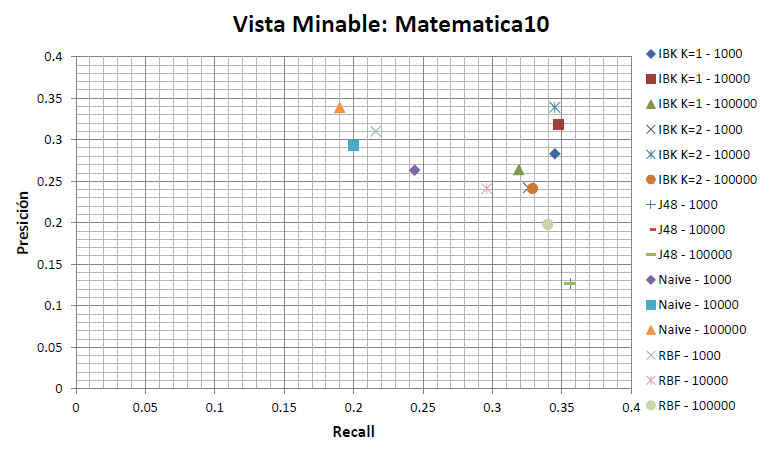
\includegraphics[scale=0.4]{matematica10}
\par\end{centering}
\caption{Precision y recall obtenidos al evaluar los clasificadores entrenados usando la vista minable Matematica10.}
\label{fig:figura8}
\end{figure}
\end{textblock}

\begin{textblock}{80}(25,170)
\begin{figure}[!htb]
\begin{centering}
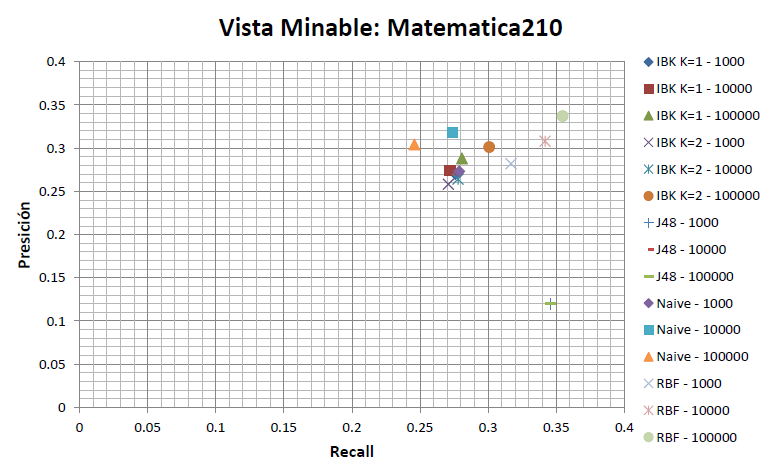
\includegraphics[scale=0.4]{matematica210}
\par\end{centering}
\caption{Precision y recall obtenidos al evaluar los clasificadores entrenados usando la vista minable Matematica210.}
\label{fig:figura9}
\end{figure}
\end{textblock}

\begin{textblock}{80}(110,170)
\begin{figure}[!htb]
\begin{centering}
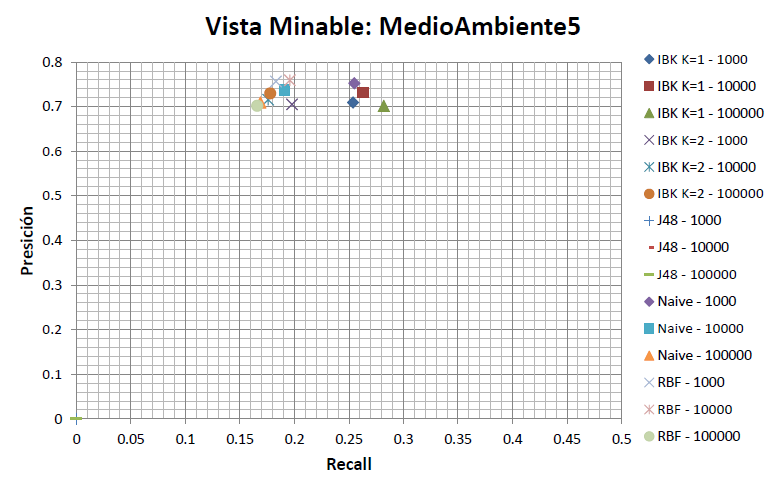
\includegraphics[scale=0.4]{medioambiente5}
\par\end{centering}
\caption{Precision y recall obtenidos al evaluar los clasificadores entrenados usando la vista minable MedioAmbiente5.}
\label{fig:figura10}
\end{figure}
\end{textblock}
\null
\clearpage

\begin{textblock}{80}(25,30)
\begin{figure}[!htb]
\begin{centering}
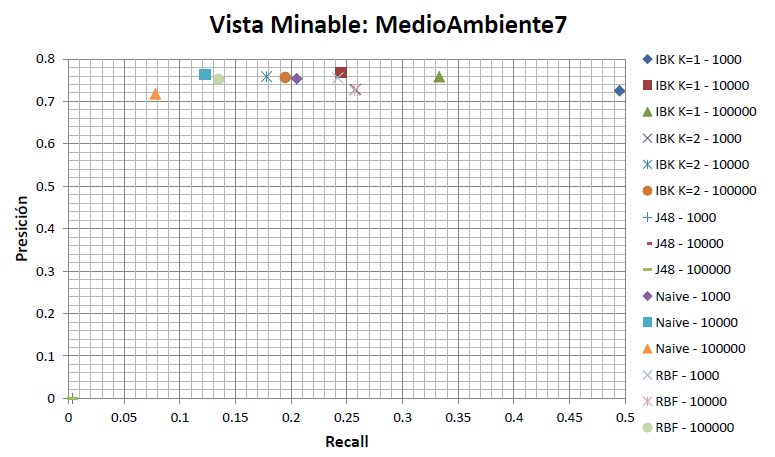
\includegraphics[scale=0.4]{medioambiente7}
\par\end{centering}
\caption{Precision y recall obtenidos al evaluar los clasificadores entrenados usando la vista minable MedioAmbiente7.}
\label{fig:figura11}
\end{figure}
\end{textblock}

\begin{textblock}{80}(110,30)
\begin{figure}[!htb]
\begin{centering}
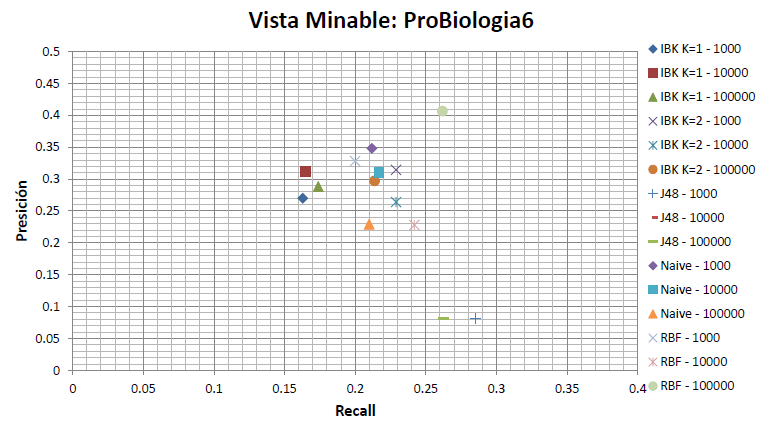
\includegraphics[scale=0.4]{probiologia6}
\par\end{centering}
\caption{Precision y recall obtenidos al evaluar los clasificadores entrenados usando la vista minable ProBiologia6.}
\label{fig:figura12}
\end{figure}
\end{textblock}

\begin{textblock}{80}(25,100)
\begin{figure}[!htb]
\begin{centering}
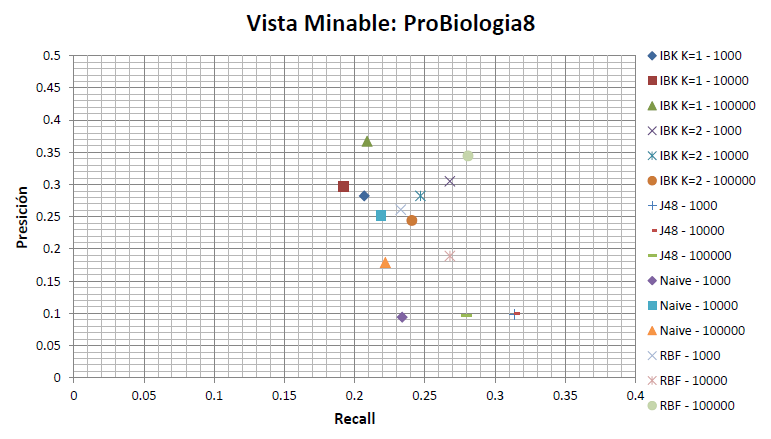
\includegraphics[scale=0.4]{probiologia8}
\par\end{centering}
\caption{Precision y recall obtenidos al evaluar los clasificadores entrenados usando la vista minable ProBiologia8.}
\label{fig:figura13}
\end{figure}
\end{textblock}

\begin{textblock}{80}(110,100)
\begin{figure}[!htb]
\begin{centering}
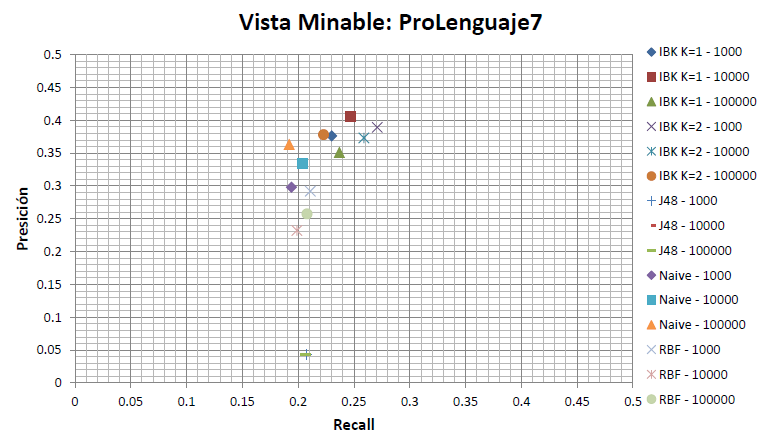
\includegraphics[scale=0.4]{prolenguaje7}
\par\end{centering}
\caption{Precision y recall obtenidos al evaluar los clasificadores entrenados usando la vista minable ProLenguaje7.}
\label{fig:figura14}
\end{figure}
\end{textblock}

\begin{textblock}{80}(25,170)
\begin{figure}[!htb]
\begin{centering}
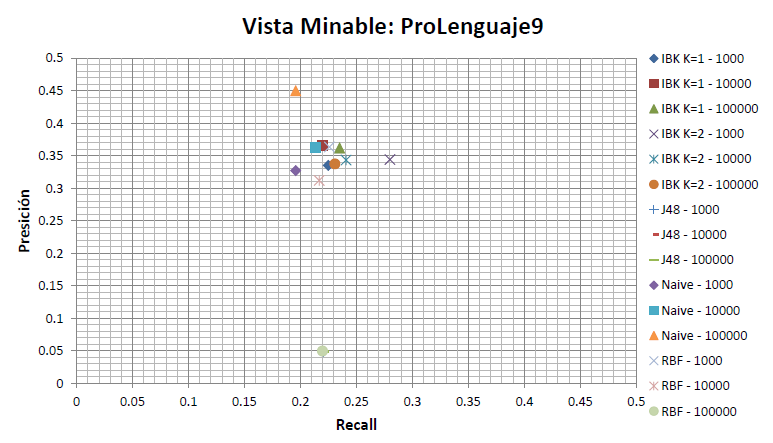
\includegraphics[scale=0.4]{prolenguaje9}
\par\end{centering}
\caption{Precision y recall obtenidos al evaluar los clasificadores entrenados usando la vista minable ProLenguaje9.}
\label{fig:figura15}
\end{figure}
\end{textblock}

\begin{textblock}{80}(110,170)
\begin{figure}[!htb]
\begin{centering}
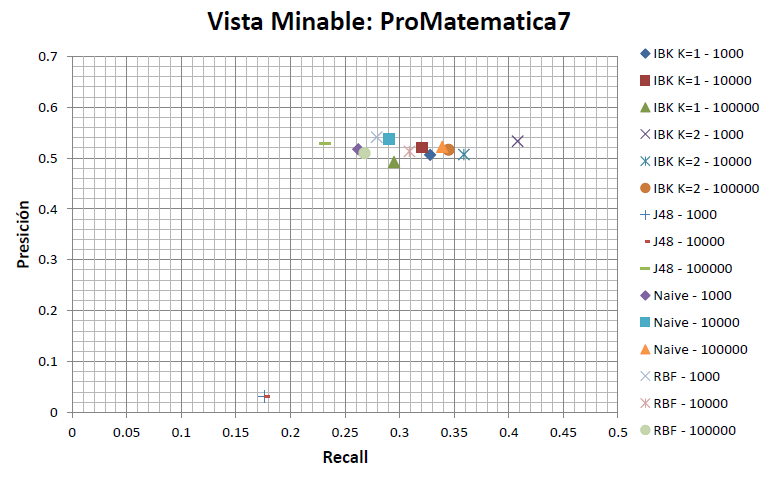
\includegraphics[scale=0.4]{promatematica7}
\par\end{centering}
\caption{Precision y recall obtenidos al evaluar los clasificadores entrenados usando la vista minable ProMatematica7.}
\label{fig:figura16}
\end{figure}
\end{textblock}
\null
\newpage
\begin{textblock}{80}(25,30)
\begin{figure}[!htb]
\begin{centering}
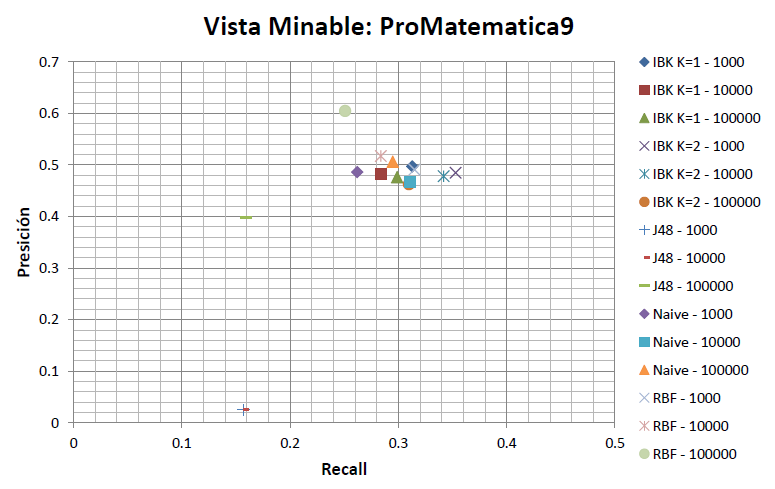
\includegraphics[scale=0.4]{promatematica9}
\par\end{centering}
\caption{Precision y recall obtenidos al evaluar los clasificadores entrenados usando la vista minable ProMatematica9.}
\label{fig:figura17}
\end{figure}
\end{textblock}

\begin{textblock}{80}(110,30)
\begin{figure}[!htb]
\begin{centering}
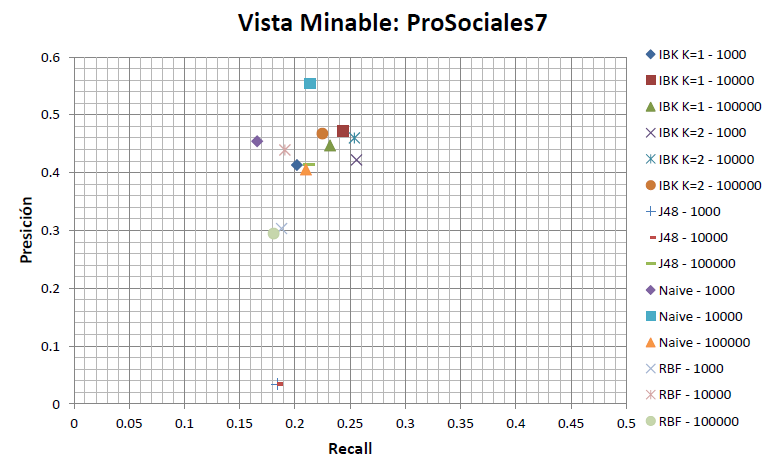
\includegraphics[scale=0.4]{prosociales7}
\par\end{centering}
\caption{Precision y recall obtenidos al evaluar los clasificadores entrenados usando la vista minable ProSociales7.}
\label{fig:figura18}
\end{figure}
\end{textblock}

\begin{textblock}{80}(25,105)
\begin{figure}[!htb]
\begin{centering}
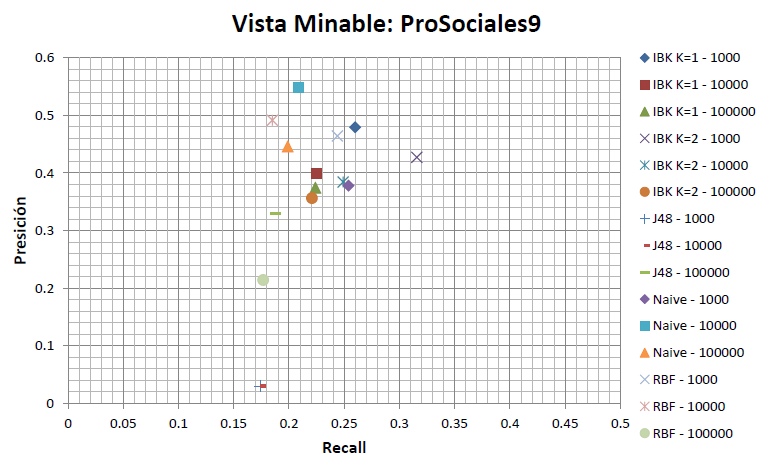
\includegraphics[scale=0.4]{prosociales9}
\par\end{centering}
\caption{Precision y recall obtenidos al evaluar los clasificadores entrenados usando la vista minable ProSociales9.}
\label{fig:figura19}
\end{figure}
\end{textblock}

\begin{textblock}{80}(110,105)
\begin{figure}[!htb]
\begin{centering}
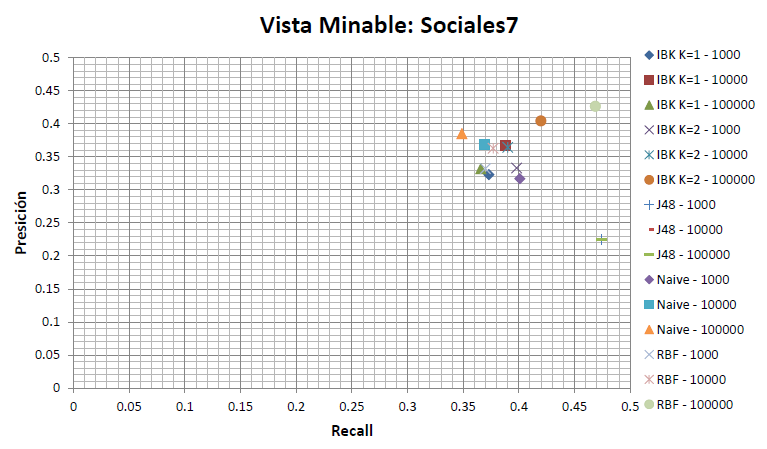
\includegraphics[scale=0.4]{sociales7}
\par\end{centering}
\caption{Precision y recall obtenidos al evaluar los clasificadores entrenados usando la vista minable Sociales7.}
\label{fig:figura20}
\end{figure}
\end{textblock}

\begin{textblock}{80}(25,180)
\begin{figure}[!htb]
\begin{centering}
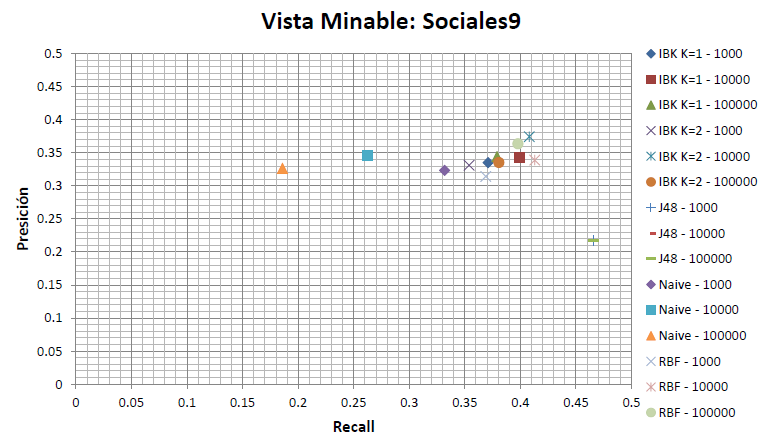
\includegraphics[scale=0.4]{sociales9}
\par\end{centering}
\caption{Precision y recall obtenidos al evaluar los clasificadores entrenados usando la vista minable Sociales9.}
\label{fig:figura21}
\end{figure}
\end{textblock}

\begin{textblock}{80}(110,180)
\begin{figure}[!htb]
\begin{centering}
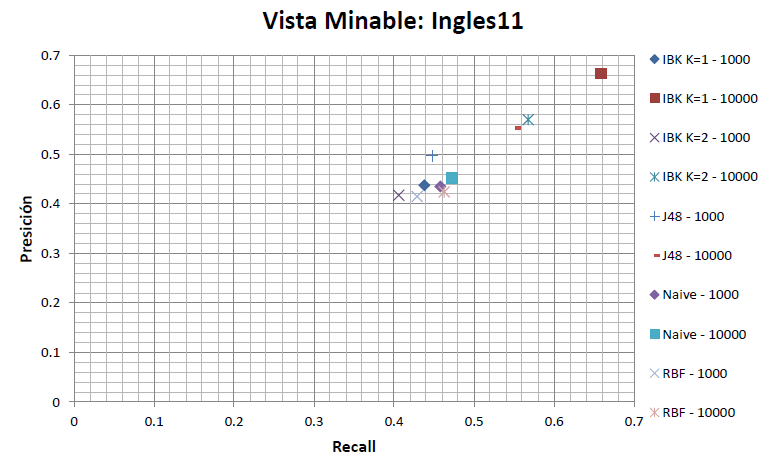
\includegraphics[scale=0.4]{ingles11}
\par\end{centering}
\caption{Precision y recall obtenidos al evaluar los clasificadores entrenados usando la vista minable Ingles11.}
\label{fig:figura22}
\end{figure}
\end{textblock}
\null
\newpage
\begin{textblock}{80}(25,30)
\begin{figure}[!htb]
\begin{centering}
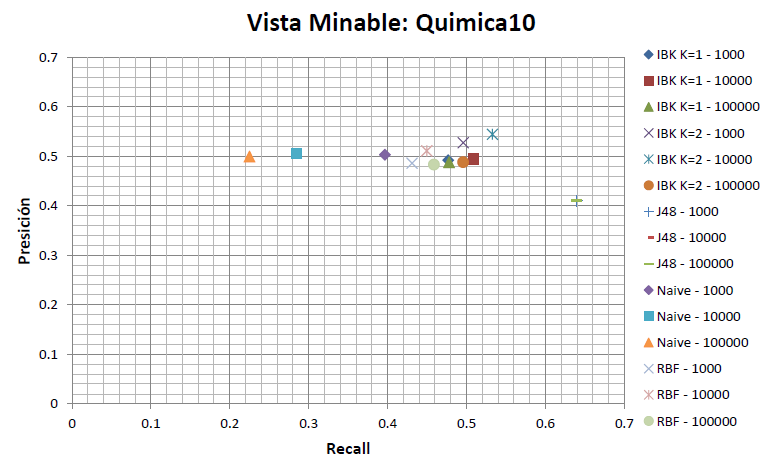
\includegraphics[scale=0.4]{quimica10}
\par\end{centering}
\caption{Precision y recall obtenidos al evaluar los clasificadores entrenados usando la vista minable Quimica10.}
\label{fig:figura23}
\end{figure}
\end{textblock}

\begin{textblock}{80}(110,30)
\begin{figure}[!htb]
\begin{centering}
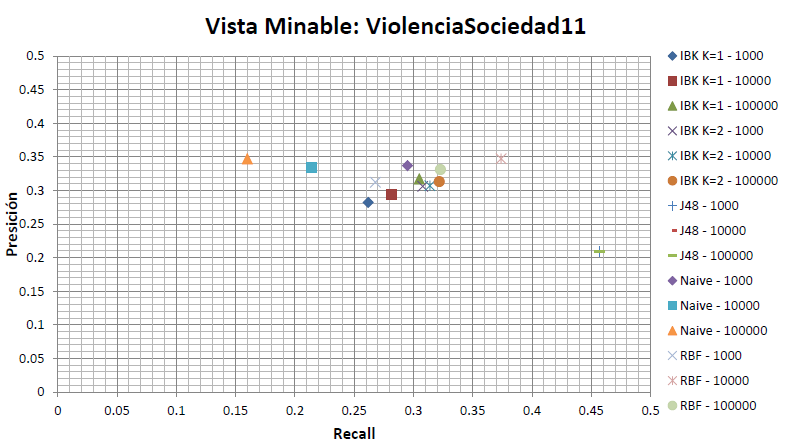
\includegraphics[scale=0.4]{violenciasociedad11}
\par\end{centering}
\caption{Precision y recall obtenidos al evaluar los clasificadores entrenados usando la vista minable ViolenciaSociedad11.}
\label{fig:figura24}
\end{figure}
\end{textblock}
\end{document}
%\include{capitulo1}
%\include{capitulo2}
%\include{capitulo3}
%\include{conclu}

\appendix
%% Cap'itulos incluidos despues del comando \appendix aparecen como ap'endices
%% de la tesis.
%\include{apendiceA}
%\include{apendiceB}
%\include{apendiceC}

%% Incluir la bibliograf'ia. Mirar el archivo "biblio.bib" para m'as detales
%% y un ejemplo.
\bibliography{biblio}

\end{document}
